% Options for packages loaded elsewhere
\PassOptionsToPackage{unicode}{hyperref}
\PassOptionsToPackage{hyphens}{url}
\documentclass[
  10pt,
]{article}
\usepackage{xcolor}
\usepackage[margin=2cm]{geometry}
\usepackage{amsmath,amssymb}
\setcounter{secnumdepth}{5}
\usepackage{iftex}
\ifPDFTeX
  \usepackage[T1]{fontenc}
  \usepackage[utf8]{inputenc}
  \usepackage{textcomp} % provide euro and other symbols
\else % if luatex or xetex
  \usepackage{unicode-math} % this also loads fontspec
  \defaultfontfeatures{Scale=MatchLowercase}
  \defaultfontfeatures[\rmfamily]{Ligatures=TeX,Scale=1}
\fi
\usepackage{lmodern}
\ifPDFTeX\else
  % xetex/luatex font selection
\fi
% Use upquote if available, for straight quotes in verbatim environments
\IfFileExists{upquote.sty}{\usepackage{upquote}}{}
\IfFileExists{microtype.sty}{% use microtype if available
  \usepackage[]{microtype}
  \UseMicrotypeSet[protrusion]{basicmath} % disable protrusion for tt fonts
}{}
\makeatletter
\@ifundefined{KOMAClassName}{% if non-KOMA class
  \IfFileExists{parskip.sty}{%
    \usepackage{parskip}
  }{% else
    \setlength{\parindent}{0pt}
    \setlength{\parskip}{6pt plus 2pt minus 1pt}}
}{% if KOMA class
  \KOMAoptions{parskip=half}}
\makeatother
\usepackage{longtable,booktabs,array}
\usepackage{calc} % for calculating minipage widths
% Correct order of tables after \paragraph or \subparagraph
\usepackage{etoolbox}
\makeatletter
\patchcmd\longtable{\par}{\if@noskipsec\mbox{}\fi\par}{}{}
\makeatother
% Allow footnotes in longtable head/foot
\IfFileExists{footnotehyper.sty}{\usepackage{footnotehyper}}{\usepackage{footnote}}
\makesavenoteenv{longtable}
\usepackage{graphicx}
\makeatletter
\newsavebox\pandoc@box
\newcommand*\pandocbounded[1]{% scales image to fit in text height/width
  \sbox\pandoc@box{#1}%
  \Gscale@div\@tempa{\textheight}{\dimexpr\ht\pandoc@box+\dp\pandoc@box\relax}%
  \Gscale@div\@tempb{\linewidth}{\wd\pandoc@box}%
  \ifdim\@tempb\p@<\@tempa\p@\let\@tempa\@tempb\fi% select the smaller of both
  \ifdim\@tempa\p@<\p@\scalebox{\@tempa}{\usebox\pandoc@box}%
  \else\usebox{\pandoc@box}%
  \fi%
}
% Set default figure placement to htbp
\def\fps@figure{htbp}
\makeatother
% definitions for citeproc citations
\NewDocumentCommand\citeproctext{}{}
\NewDocumentCommand\citeproc{mm}{%
  \begingroup\def\citeproctext{#2}\cite{#1}\endgroup}
\makeatletter
 % allow citations to break across lines
 \let\@cite@ofmt\@firstofone
 % avoid brackets around text for \cite:
 \def\@biblabel#1{}
 \def\@cite#1#2{{#1\if@tempswa , #2\fi}}
\makeatother
\newlength{\cslhangindent}
\setlength{\cslhangindent}{1.5em}
\newlength{\csllabelwidth}
\setlength{\csllabelwidth}{3em}
\newenvironment{CSLReferences}[2] % #1 hanging-indent, #2 entry-spacing
 {\begin{list}{}{%
  \setlength{\itemindent}{0pt}
  \setlength{\leftmargin}{0pt}
  \setlength{\parsep}{0pt}
  % turn on hanging indent if param 1 is 1
  \ifodd #1
   \setlength{\leftmargin}{\cslhangindent}
   \setlength{\itemindent}{-1\cslhangindent}
  \fi
  % set entry spacing
  \setlength{\itemsep}{#2\baselineskip}}}
 {\end{list}}
\usepackage{calc}
\newcommand{\CSLBlock}[1]{\hfill\break\parbox[t]{\linewidth}{\strut\ignorespaces#1\strut}}
\newcommand{\CSLLeftMargin}[1]{\parbox[t]{\csllabelwidth}{\strut#1\strut}}
\newcommand{\CSLRightInline}[1]{\parbox[t]{\linewidth - \csllabelwidth}{\strut#1\strut}}
\newcommand{\CSLIndent}[1]{\hspace{\cslhangindent}#1}
\setlength{\emergencystretch}{3em} % prevent overfull lines
\providecommand{\tightlist}{%
  \setlength{\itemsep}{0pt}\setlength{\parskip}{0pt}}
\usepackage{bookmark}
\IfFileExists{xurl.sty}{\usepackage{xurl}}{} % add URL line breaks if available
\urlstyle{same}
\hypersetup{
  pdftitle={Memorised Blades: data leakage inflates wind-turbine blade defect benchmarks, and tuning on them rewards it},
  pdfauthor={Bhavya Goel},
  hidelinks,
  pdfcreator={LaTeX via pandoc}}

\title{Memorised Blades: data leakage inflates wind-turbine blade defect
benchmarks, and tuning on them rewards it}
\author{Bhavya Goel}
\date{Draft of 8 November 2026. Affiliation and contact to be added.}

\begin{document}
\maketitle
\begin{abstract}
Public benchmarks for wind-turbine blade defect detection report 85--92
mAP50. We audit the three most used, WTBD, Wind Surface Defect and
WTBlade-Defect, with image retrieval, geometric verification and pixel
correlation. We find that 78\%, 84\% and 92\% of their official test
images have a near-copy or same-scene image in the training split,
because the datasets were augmented or tiled before a random split. A
generic foundation detector (RF-DETR-M) with a standard recipe scores
90.4 mAP50 on WTBD's official split and 87.2 on WTBlade-Defect's, above
the published BladeYOLO on the latter (85.8), though below it on Wind
Surface (81.0 vs 86.5). The same runs lose 24 and 40 points on the Wind
Surface and WTBlade-Defect test images without a training twin: on
WTBlade-Defect they score 98.2 on copies of training frames and 50.4 on
images with no twin. Trained with the same recipe on a scene-grouped
split of the same WTBD images, the detector falls from 90.4 / 61.2 to
55.3 / 33.2 mAP50 / mAP50-95. A single step of recipe tuning against the
official numbers raised the score on leaked images and lowered it on
unseen ones on all three datasets, so leaderboard tuning on these splits
rewards memorisation. We release two leak-free benchmarks with
scene-level intervals. On them, frozen DINOv3 features account for the
whole advantage of a modern YOLO variant at every label budget, and its
deformable, selective-scan and loss components add nothing measurable.
Fine-tuned RF-DETR leads on WTBD-group but not on WTBlade-group. We
measure an annotation self-consistency ceiling of 84--87\% on exact
copies, a factor-of-two dependence of low-label results on which scenes
are labelled, and a failure of conformal recall guarantees calibrated on
seen scenes (31.5\% missed against a promised 10\%). Finally, more data
from other sources does not replace target labels: a detector trained on
26,065 twin-free images from other datasets reaches 17.7 class-agnostic
AP50 on WTBD-group test, against 72.9 for 745 target images, and 2.4
against 51.7 on WTBlade-group. A ledger of our pre-registered method
tests, most of them failures, shows that the usual add-ons do not close
the leak-free gap.
\end{abstract}

\section{Introduction}\label{introduction}

Blade inspection by drone is one of the more mature applications of
defect detection, and the published numbers suggest a nearly solved
problem. BladeYOLO {[}\citeproc{ref-bladeyolo}{1}{]} reports 86.5 / 57.4
mAP50 / mAP50-95 on Wind Surface Defect and 85.8 / 74.6 on
WTBlade-Defect, and other recent architectures report similar levels
{[}\citeproc{ref-gfdyolox}{2}--\citeproc{ref-kgpyolo}{4}{]}. This work
began as an attempt to reproduce one of those results and build on it.
The closest faithful reimplementation we could build stopped at about
52.6 / 28, and our next model reached 78.2 / 46.9, until we found that
three-quarters of the validation images had a near-identical twin in the
training set. That finding changed the question from ``how do we beat
this number?'' to three others:

\begin{enumerate}
\def\labelenumi{\arabic{enumi}.}
\tightlist
\item
  What do these benchmarks measure?
\item
  How much of a reported score is memorisation of scenes seen in
  training?
\item
  Once leakage is removed, what actually helps, and what limits the
  score?
\end{enumerate}

We answer them with an end-to-end audit and about two months of
controlled experiments. Our contributions are measurements, not a new
architecture. We tried to find a method that survives a second dataset,
and did not; §~9 reports those attempts.

\begin{itemize}
\tightlist
\item
  \textbf{A leakage audit of the public blade benchmarks} (Table~1,
  Fig.~3). A literature check found no earlier audit of these datasets.
  The check was not exhaustive.
\item
  \textbf{The size of the inflation}, on the same detector and recipe:
  leaked against no-twin test images (Table~3), and official against
  scene-grouped splits (Table~4, Fig.~10).
\item
  \textbf{Evidence that tuning on leaky benchmarks selects for
  memorisation} (Table~5, Fig.~8). This analysis is post hoc and covers
  one tuning step.
\item
  \textbf{Two leak-free benchmarks}, WTBD-group and WTBlade-group, with
  audited splits, scene groups and a scene bootstrap (§~4), and
  baselines for RF-DETR, a DINOv3-fused YOLO and stock YOLO12-L
  (Table~7).
\item
  \textbf{Controlled ablations} that attribute the low-label and
  full-label advantage of a DINOv3-fused YOLO to the frozen features
  alone (Table~8, Fig.~12).
\item
  \textbf{Measured ceilings}: annotator self-consistency, box
  granularity, subset luck and error anatomy (§~7).
\item
  \textbf{A leave-one-dataset-out test} with twin-free pools (§~8), and
  a recall-guarantee failure caused by leaked calibration (Table~6).
\item
  \textbf{A ledger of the method tests we ran or formally gated},
  including the failures (Table~21), and an account of how our own early
  numbers were wrong (§~10).
\end{itemize}

The authors of the papers we discuss followed common practice, which is
to augment and then split at random. Our argument is about the protocol,
not about them. We cannot say that any specific published number is due
to memorisation, because those splits were not published.

Fig.~1 shows how the parts of the study fit together.

\begin{figure}
\centering
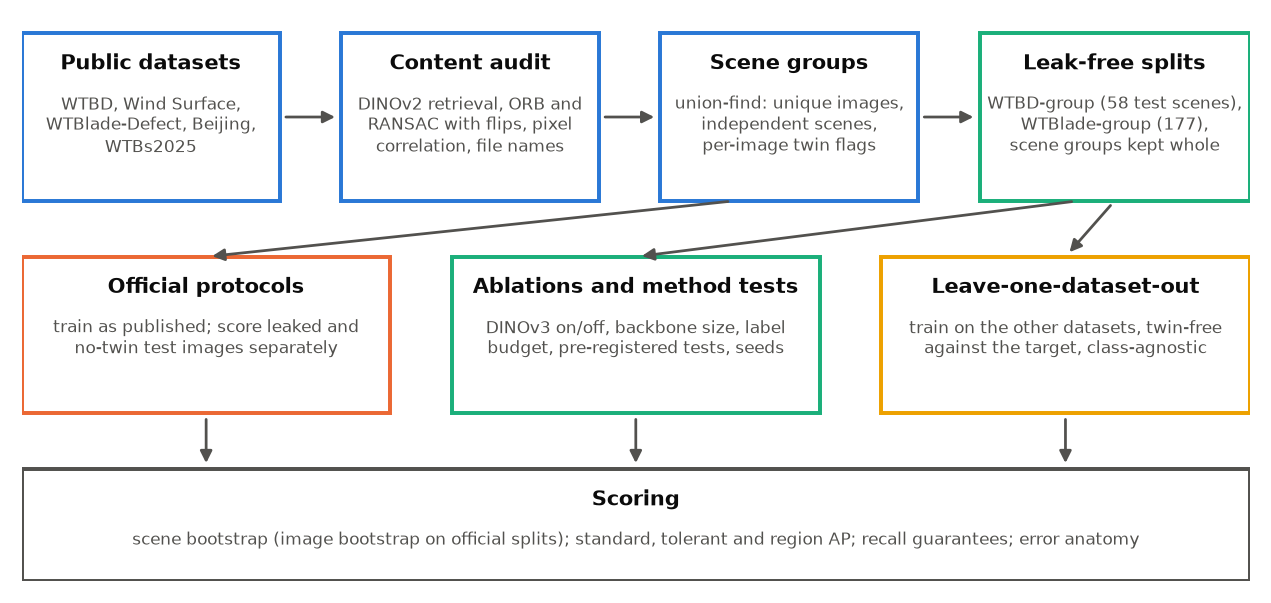
\includegraphics[width=0.92\linewidth,height=\textheight,keepaspectratio,alt={Figure 1. Overview of the study. The audit produces scene groups and per-image twin flags. These define the leak-free splits and the leaked and no-twin subsets of the official test sets. All experiments share the same scoring.}]{figures/fig7_pipeline.png}
\caption{Figure 1. Overview of the study. The audit produces scene
groups and per-image twin flags. These define the leak-free splits and
the leaked and no-twin subsets of the official test sets. All
experiments share the same scoring.}
\end{figure}

\section{Related work}\label{related-work}

\textbf{Blade defect detection.} Most work adapts YOLO variants with
attention, wavelet, deformable or Mamba-style modules
{[}\citeproc{ref-bladeyolo}{1}--\citeproc{ref-kgpyolo}{4}{]}, and
several build on the DTU NordTank drone inspection imagery
{[}\citeproc{ref-shihavuddin}{5}, \citeproc{ref-foster}{6}{]}. BladeYOLO
fuses frozen DINOv3 ViT-S/16 features into YOLOv12-L
{[}\citeproc{ref-bladeyolo}{1}, \citeproc{ref-yolov12}{7}{]}, close in
spirit to DINO-YOLO in civil engineering
{[}\citeproc{ref-dinoyolo}{8}{]}. Data-descriptor papers have added new
sets, notably WTBD {[}\citeproc{ref-wtbd}{9}{]} and WTBs2025
{[}\citeproc{ref-wtbs2025}{10}{]}. Training-free language-model
inspection {[}\citeproc{ref-seeingunseen}{11}{]} and box-to-mask
supervision {[}\citeproc{ref-boxes2pixels}{12}{]} are recent directions,
and we have not tested those specific claims on a leak-free split.

\textbf{Leakage and near-duplicates.} Near-duplicates between train and
test are documented for CIFAR {[}\citeproc{ref-barz}{13}{]}, geospatial
mapping data {[}\citeproc{ref-adimoolam}{14}{]} and more generally as a
source of irreproducible machine-learning results
{[}\citeproc{ref-kapoor}{15}{]}; and a fresh test set can show lower
accuracy than a reused one {[}\citeproc{ref-recht}{16}{]}. Long-tail
memorisation is a mechanism by which rare test examples are classified
correctly through similar training examples
{[}\citeproc{ref-feldman}{17}{]}. We apply this line of work to blade
defect benchmarks, and add a same-detector measurement of what the leak
buys and what tuning on it rewards.

\textbf{Foundation detectors.} RF-DETR {[}\citeproc{ref-rfdetr}{18}{]}
fine-tunes DINOv2 {[}\citeproc{ref-dinov2}{19}{]} end to end and is
strong on Roboflow100-VL {[}\citeproc{ref-rf100vl}{20}{]}. DINOv3
{[}\citeproc{ref-dinov3}{21}{]} offers frozen dense features.
Fine-tuning can distort pretrained features under distribution shift
{[}\citeproc{ref-lpft}{22}{]}.

\textbf{Label noise and granularity in evaluation.} TedEval
{[}\citeproc{ref-tedeval}{23}{]} handles split and merged instances in
text detection. Box-annotation noise has been studied in detection
evaluation {[}\citeproc{ref-murrugarra}{24}{]} and in repeated labels
{[}\citeproc{ref-tschirschwitz}{25}{]}, and box regression can model its
own uncertainty {[}\citeproc{ref-klloss}{26}{]}. We measure the same
kind of ambiguity from accidental repeated labels: independently
annotated copies of the same image.

\textbf{Calibration and subset variance.} Conformal risk control
{[}\citeproc{ref-crc}{27}{]} gives distribution-free guarantees under
exchangeability, and has been applied to detection
{[}\citeproc{ref-andeol}{28}{]}. Few-shot detection results vary
strongly with the sampled shots {[}\citeproc{ref-tfa}{29}{]}; we measure
that variance in a realistic low-label setting and test label-free
selection {[}\citeproc{ref-freesel}{30}{]}.

\textbf{Multi-dataset and domain generalisation.} Multi-dataset
detection with partitioned label spaces
{[}\citeproc{ref-multidataset}{31}{]} and training-domain model
selection {[}\citeproc{ref-domainbed}{32}{]} inform our G27 and G28
designs. Copy-paste {[}\citeproc{ref-copypaste}{33}{]} is a known
augmentation, and we test it only as a recipe component.

\section{Datasets and the leakage audit}\label{sec:audit}

\subsection{Datasets}\label{datasets}

We work with the official classes of each dataset, because the
taxonomies conflict (below). Fig.~2 shows random labelled examples and
Table~1 summarises the audit.

\begin{figure}
\centering
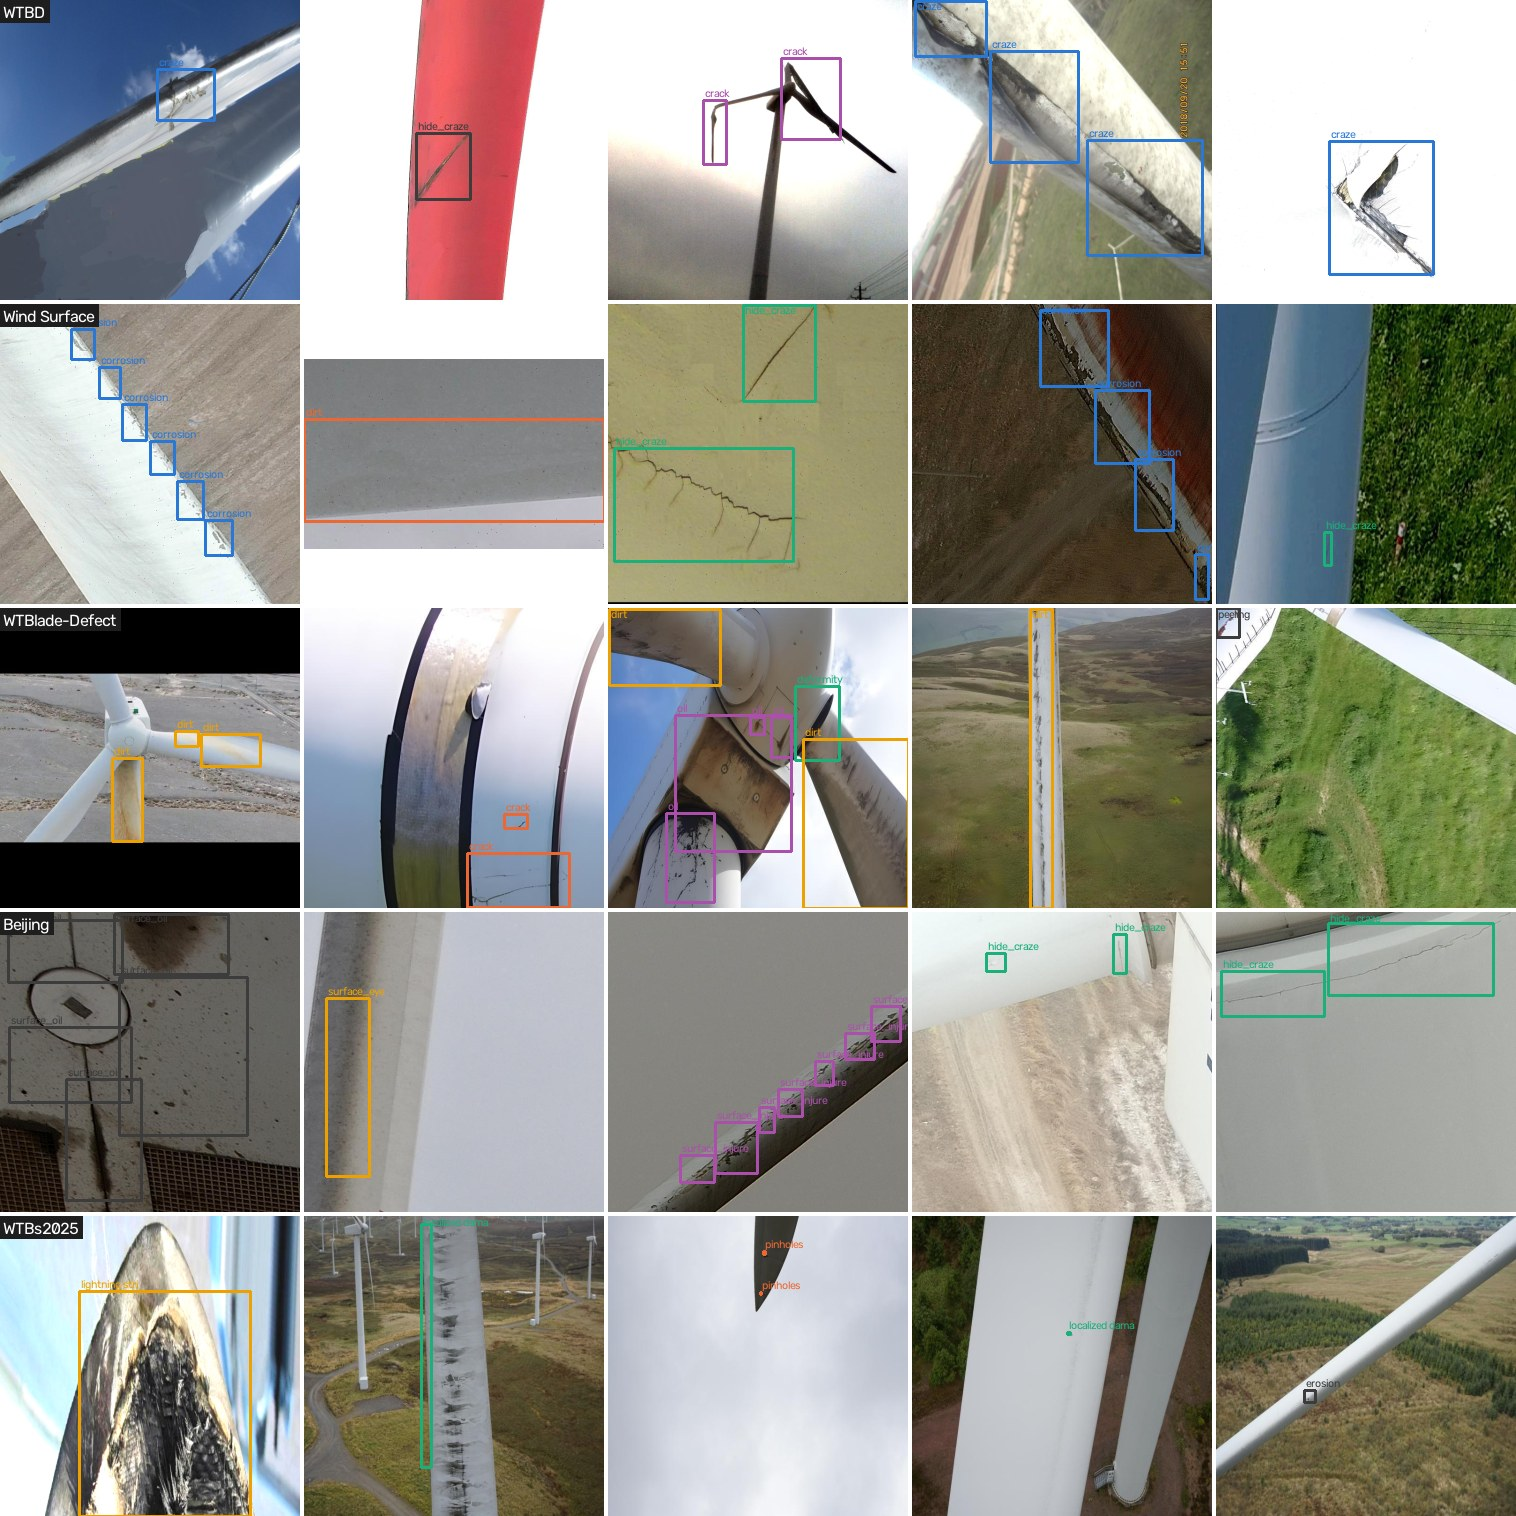
\includegraphics[width=0.88\linewidth,height=\textheight,keepaspectratio,alt={Figure 2. Random labelled training images from each dataset (fixed seed; the first three in each row are required to show a class not yet shown). Colour marks the class within a row. Note the differences in viewpoint and box style, from close-ups with one box (WTBD) to chains of small boxes along an edge (Wind Surface, Beijing) and very small boxes (WTBs2025). Black squares in WTBlade-Defect are the Roboflow export's offline cutout augmentation. Source licences are in §~13.}]{figures/fig8_dataset_gallery.jpg}
\caption{Figure 2. Random labelled training images from each dataset
(fixed seed; the first three in each row are required to show a class
not yet shown). Colour marks the class within a row. Note the
differences in viewpoint and box style, from close-ups with one box
(WTBD) to chains of small boxes along an edge (Wind Surface, Beijing)
and very small boxes (WTBs2025). Black squares in WTBlade-Defect are the
Roboflow export's offline cutout augmentation. Source licences are in
§~13.}
\end{figure}

\begin{longtable}[]{@{}
  >{\raggedright\arraybackslash}p{(\linewidth - 12\tabcolsep) * \real{0.1429}}
  >{\raggedright\arraybackslash}p{(\linewidth - 12\tabcolsep) * \real{0.1429}}
  >{\raggedright\arraybackslash}p{(\linewidth - 12\tabcolsep) * \real{0.1429}}
  >{\raggedright\arraybackslash}p{(\linewidth - 12\tabcolsep) * \real{0.1429}}
  >{\raggedright\arraybackslash}p{(\linewidth - 12\tabcolsep) * \real{0.1429}}
  >{\raggedright\arraybackslash}p{(\linewidth - 12\tabcolsep) * \real{0.1429}}
  >{\raggedright\arraybackslash}p{(\linewidth - 12\tabcolsep) * \real{0.1429}}@{}}
\caption{Table 1. The three benchmarks and their official splits. Unique
images and scenes are from the content-based audit. A \emph{twin} is a
near-copy or same-scene image among the images the run trained
on.}\tabularnewline
\toprule\noalign{}
\begin{minipage}[b]{\linewidth}\raggedright
dataset
\end{minipage} & \begin{minipage}[b]{\linewidth}\raggedright
files
\end{minipage} & \begin{minipage}[b]{\linewidth}\raggedright
unique images
\end{minipage} & \begin{minipage}[b]{\linewidth}\raggedright
independent scenes
\end{minipage} & \begin{minipage}[b]{\linewidth}\raggedright
official split (train / val / test)
\end{minipage} & \begin{minipage}[b]{\linewidth}\raggedright
test images with a training twin
\end{minipage} & \begin{minipage}[b]{\linewidth}\raggedright
how the twin arises
\end{minipage} \\
\midrule\noalign{}
\endfirsthead
\toprule\noalign{}
\begin{minipage}[b]{\linewidth}\raggedright
dataset
\end{minipage} & \begin{minipage}[b]{\linewidth}\raggedright
files
\end{minipage} & \begin{minipage}[b]{\linewidth}\raggedright
unique images
\end{minipage} & \begin{minipage}[b]{\linewidth}\raggedright
independent scenes
\end{minipage} & \begin{minipage}[b]{\linewidth}\raggedright
official split (train / val / test)
\end{minipage} & \begin{minipage}[b]{\linewidth}\raggedright
test images with a training twin
\end{minipage} & \begin{minipage}[b]{\linewidth}\raggedright
how the twin arises
\end{minipage} \\
\midrule\noalign{}
\endhead
\bottomrule\noalign{}
\endlastfoot
WTBD {[}\citeproc{ref-wtbd}{9}{]} & 1,065 & 597 & \textasciitilde550 &
745 / 159 / 161 & \textbf{125 / 161 (78\%)} & duplicate and augmented
copies of one photo, split at random (seed 42) \\
Wind Surface Defect {[}\citeproc{ref-gfdyolox}{2}{]}, used by BladeYOLO
& 3,570 & 954 & \textbf{81} & 2,856 / 714 (val = test) & \textbf{600 /
714 (84\%)} pixel twins (corr ≥ 0.99) & 1,785 originals plus one
augmented copy each (550 pairs split across train and val); up to 44
tiles per drone photo (386 of 882 photos on both sides) \\
WTBlade-Defect {[}\citeproc{ref-fengche}{34}{]}, used by BladeYOLO &
10,660 & 1,146 & 803 & 9,010 / 1,097 / 553 & \textbf{499 / 542 (92\%)}
same scene; \textbf{360 (66\%)} copies of a training frame & about 3
Roboflow augmentation copies per source frame; consecutive drone-video
frames \\
\end{longtable}

\subsection{Audit method}\label{audit-method}

Files cannot be compared by name or hash, because the copies are
flipped, rotated, recoloured or re-encoded. We combine several signals:

\begin{enumerate}
\def\labelenumi{\arabic{enumi}.}
\tightlist
\item
  \textbf{Retrieval:} DINOv2 embeddings {[}\citeproc{ref-dinov2}{19}{]},
  cosine nearest neighbours.
\item
  \textbf{Geometric verification:} flip-aware ORB matching with a RANSAC
  similarity transform, at least 25 inliers.
\item
  \textbf{Pixel twins:} correlation at 48 px over the eight flips and
  rotations, at least 0.99.
\item
  \textbf{Provenance from file names:} Roboflow source prefixes,
  \texttt{DJI\_xxxx\_r\_c} tile coordinates, and \texttt{\_0} /
  \texttt{\_1} pairs.
\item
  \textbf{Grouping:} union-find over all of the above, with DINOv2
  cosine ≥ 0.93 counted as same scene. Deduplication is non-chaining, so
  that a chain of weak matches cannot merge unrelated images.
\end{enumerate}

Example sheets were checked by eye for every dataset and outcome. On
Wind Surface the first pixel comparison, flips only, found 532 of 714
validation images (75\%); adding rotations and restricting to the images
actually trained on gives 600 (84\%). The Wind Surface ``no twin''
subset has no near-identical copy in training, but most of it comes from
drone photos with other tiles in training, so it is cleaner rather than
leak-free.

Fig.~3 shows test images and their training twins, drawn at random.

\begin{figure}
\centering
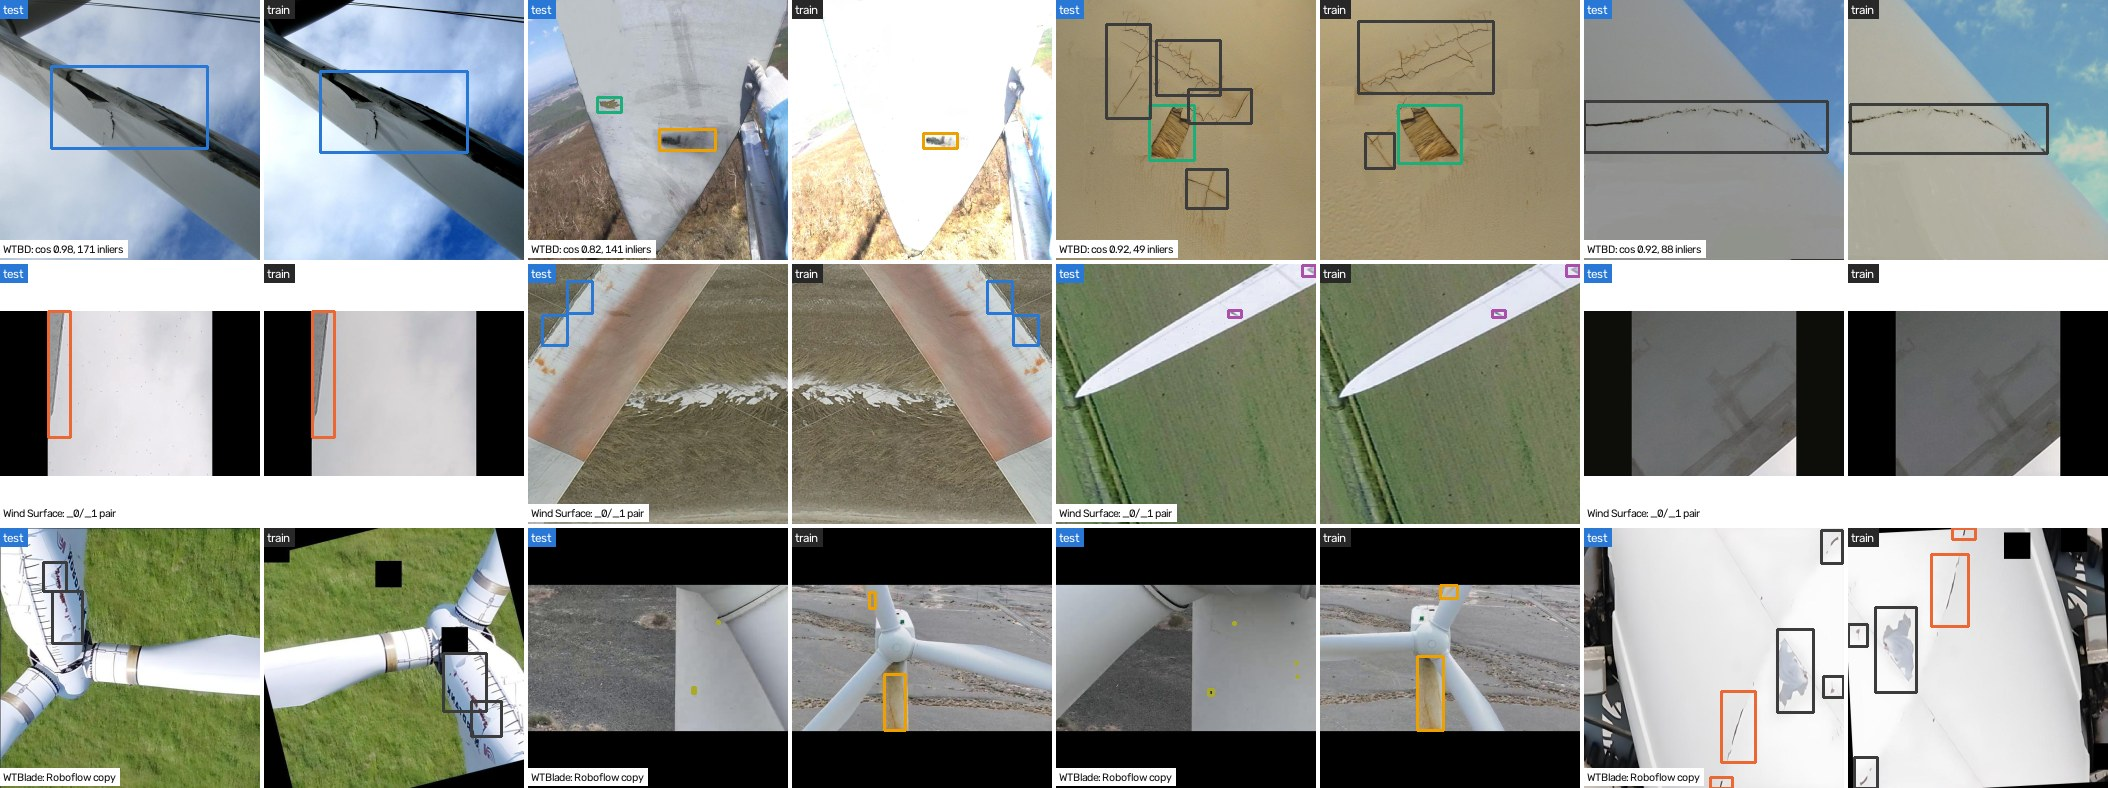
\includegraphics[width=1\linewidth,height=\textheight,keepaspectratio,alt={Figure 3. Official test images (blue tag) next to their training twins (black tag), drawn at random with a fixed seed from the leaked subsets. Labels are drawn as supplied. Row 1: WTBD, with DINOv2 cosine and ORB inliers. Row 2: Wind Surface \_0 / \_1 pairs split across the partition. Row 3: WTBlade-Defect Roboflow copies of one source frame.}]{figures/fig10_twins.jpg}
\caption{Figure 3. Official test images (blue tag) next to their
training twins (black tag), drawn at random with a fixed seed from the
leaked subsets. Labels are drawn as supplied. Row 1: WTBD, with DINOv2
cosine and ORB inliers. Row 2: Wind Surface \texttt{\_0} / \texttt{\_1}
pairs split across the partition. Row 3: WTBlade-Defect Roboflow copies
of one source frame.}
\end{figure}

\subsection{What the file counts hide}\label{what-the-file-counts-hide}

File count is a poor guide to the information in a dataset (Fig.~4).
Wind Surface's 3,570 files come from about 81 independent scenes, and
all \texttt{surface\_eye} boxes (412 in the raw files, 103 after
deduplication) come from tiles of a single photo. Any
\texttt{surface\_eye} score on the original split, including published
ones, was measured on tiles of a training photo. WTBD has far fewer
files and far more independent scenes per class. Three more findings
limit what can be merged:

\begin{itemize}
\tightlist
\item
  \textbf{Same-named classes do not match across datasets.} Mutual crop
  retrieval between same-named classes is at most 0.33, apart from the
  two Beijing exports, which are the same data.
\item
  \textbf{Datasets overlap under other names.} WTBs2025 shares 1,499
  images with WTBlade-Defect under different class names (peeling →
  erosion). Beijing contains WTBD test photos.
\item
  \textbf{Licences are not what the export pages say.} ``NORDTANK'' is
  legible on many WTBlade-Defect nacelles, so the set contains DTU
  imagery {[}\citeproc{ref-shihavuddin}{5}{]}, which is CC BY-NC, while
  its Roboflow page states CC BY 4.0. It also contains synthetic
  copy-paste images.
\end{itemize}

\begin{figure}
\centering
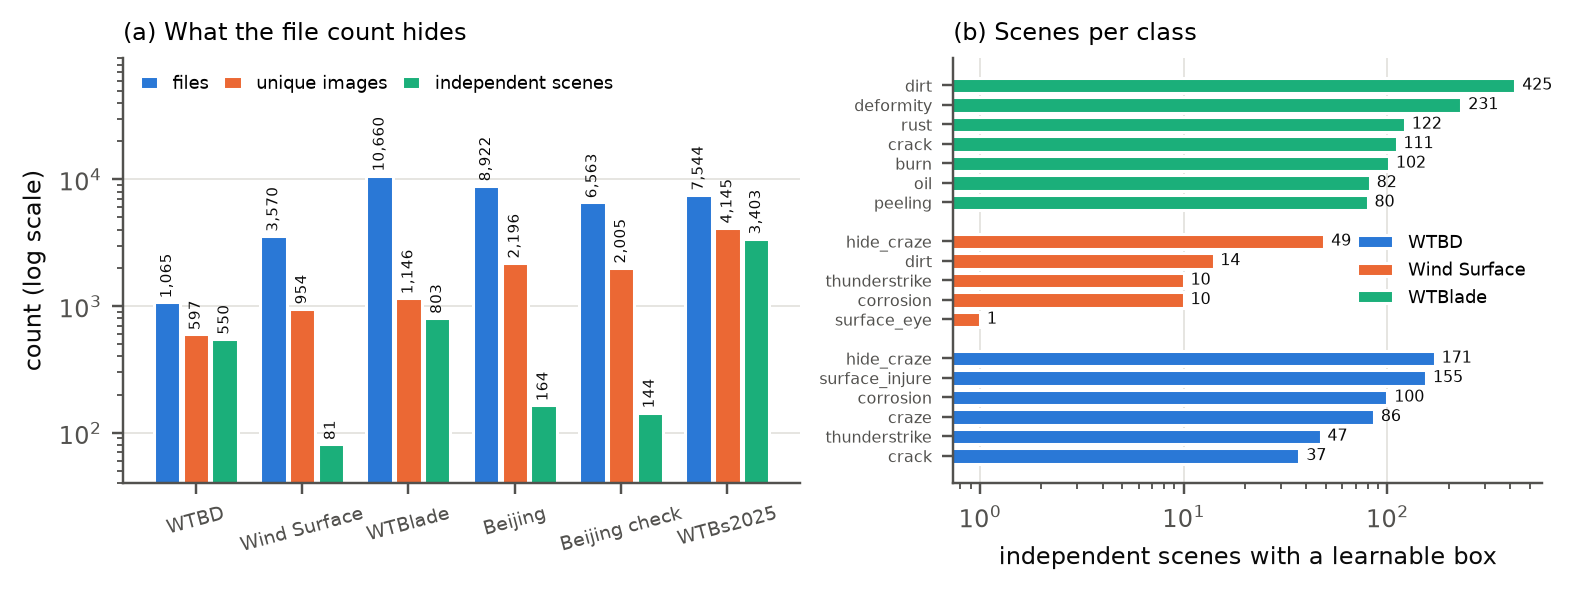
\includegraphics[width=0.96\linewidth,height=\textheight,keepaspectratio,alt={Figure 4. Effective size. (a) Files, unique images and independent scenes per dataset. (b) Independent scenes with a learnable box, per class. A single scene supports Wind Surface's surface\_eye.}]{figures/fig9_effective_size.png}
\caption{Figure 4. Effective size. (a) Files, unique images and
independent scenes per dataset. (b) Independent scenes with a learnable
box, per class. A single scene supports Wind Surface's
\texttt{surface\_eye}.}
\end{figure}

The same augment-then-split pattern appears in other published work: 130
DTU images expanded to 780 and then split 624 / 78 / 78
{[}\citeproc{ref-kgpyolo}{4}{]}, and CLAHE copies with a random 60 / 40
split of repeated shots of one turbine {[}\citeproc{ref-gayolo}{3}{]}.
BladeYOLO's WTBlade numbers use its authors' own 9:1 re-split of 5,326
images, which is not public {[}\citeproc{ref-bladeyolo}{1}{]}.

\section{Leak-free benchmarks, models and
evaluation}\label{sec:benchmarks}

\subsection{Splits}\label{splits}

\textbf{WTBD-group.} The 1,065 WTBD images are split by scene into 745 /
159 / 161 images (the official sizes), with 1,109 / 240 / 235 boxes and
224 / 60 / 58 scene groups. The split was audited until no held-out
image matched train under DINOv2 and ORB verification. Fractions of 25\%
and 50\% are nested subsets of training scenes.

\textbf{WTBlade-group.} From 10,527 WTBlade-Defect images (133 that
match WTBD are left out, so the benchmarks share nothing), we form 841
groups from 2,791 source frames, verified pairs and DINOv2 neighbours. A
class-stratified 70 / 15 / 15 split over groups converged with no
held-out or train match after 11 rounds of the audit. We keep one image
per source frame, giving 2,136 / 323 / 332 frames, 5,237 / 729 / 748
boxes, and 177 test scenes, with all seven classes in every split.

\textbf{A residual leak in our own splits.} While building a later pool
we added the pixel test to our audit and ran it on these splits. It
found copies that DINOv2 and ORB had missed: 6 of 161 test and 6 of 159
validation images on WTBD-group, and 1 of 332 and 1 of 323 on
WTBlade-group (Fig.~5). All six WTBD-group test pairs are real copies by
eye, re-exposed, darkened, tinted or rotated. Rescoring 116 cached
WTBD-group runs without those images changes mAP50-95 by −0.62 on
average (range −1.09 to +0.33) and mAP50 by −0.70, and 20 WTBlade-group
runs by ±0.03. Our leak-free numbers are therefore inflated by under a
point. We kept the splits unchanged, so that every comparison stays like
for like, and report the G27 and G28 decisions both ways (§~9, §~8).
Neither changes. So a leak-free split needs the pixel test next to scene
grouping, and ``audited'' is only as good as the audit.

\begin{figure}
\centering
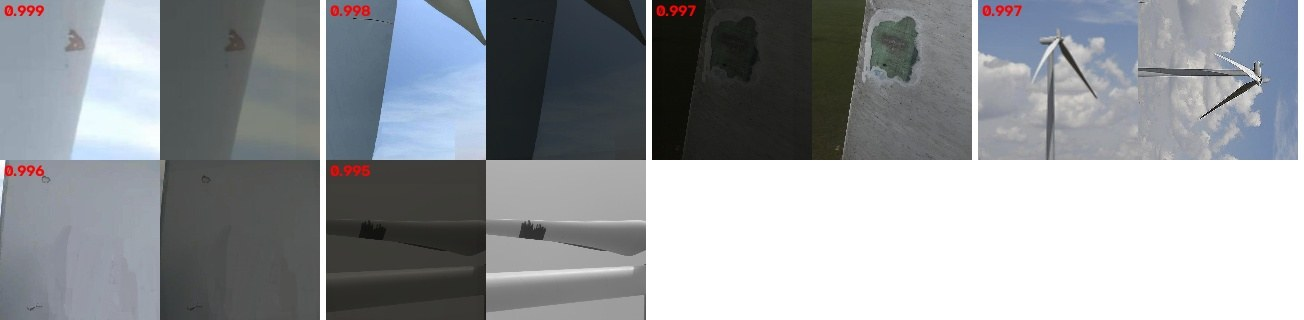
\includegraphics[width=0.78\linewidth,height=\textheight,keepaspectratio,alt={Figure 5. The residual leak in our WTBD-group test set: each pair is a test image and its pixel twin in train, with the correlation. Photometric copies defeat DINOv2 + ORB grouping.}]{figures/fig28_residual_twins.jpg}
\caption{Figure 5. The residual leak in our WTBD-group test set: each
pair is a test image and its pixel twin in train, with the correlation.
Photometric copies defeat DINOv2 + ORB grouping.}
\end{figure}

\subsection{Models and recipes}\label{models-and-recipes}

\begin{itemize}
\tightlist
\item
  \textbf{YOLO12-L:} COCO-pretrained, stock, CIoU loss, AdamW (lr 0.001,
  weight decay 0.01), cosine schedule, mosaic. 150 epochs on WTBD and 50
  on WTBlade-group.
\item
  \textbf{BladeYOLO-v2:} our model, on the same recipe. A
  COCO-pretrained YOLOv12-L {[}\citeproc{ref-yolov12}{7}{]} with three
  zero-initialised residual additions, so that training starts exactly
  at the pretrained detector: frozen DINOv3
  {[}\citeproc{ref-dinov3}{21}{]} features fused at P3 / P4 / P5,
  deformable refinement at P3 / P4 {[}\citeproc{ref-dcnv2}{35}{]}, and
  four-direction selective scan at P5 {[}\citeproc{ref-vmamba}{36},
  \citeproc{ref-mamba}{37}{]}; WIoU v3 loss
  {[}\citeproc{ref-wiou}{38}{]}. 53.7 M parameters with ViT-S/16.
\item
  \textbf{RF-DETR-M:} \texttt{rfdetr} 1.11.2
  {[}\citeproc{ref-rfdetr}{18}{]}, fine-tuned end to end from its COCO
  checkpoint. Batch 4 × accumulation 4 (effective 16), cosine schedule,
  EMA checkpoint selected on validation. WTBD at 768 px for 100 epochs;
  WTBlade at 640 px for 60 epochs.
\end{itemize}

Runs used Kaggle Tesla T4 (fp16 mixed precision) and one A100 (bf16).
All G27 seed-1 runs were on the A100 and seed-0 runs on Kaggle, so every
pair of arms within a seed shares hardware.

\subsection{Evaluation}\label{evaluation}

\textbf{Selection and reporting.} Model selection uses validation only,
and results are reported on test. Wind Surface has no separate test
split, so we carve a seeded 10\% of train for validation.

\textbf{Evaluators.} We use a 101-point COCO-style evaluator
{[}\citeproc{ref-coco}{39}{]} (\texttt{tools/bootstrap\_ci.py}). On
identical predictions it agrees with Ultralytics'
\texttt{ap\_per\_class} within 0.4 points on every run and subset, so
gaps to published figures are not an artefact of the metric.
Ultralytics' \texttt{val} reports differ by 1--2.5 points from cached
predictions because of its rectangular-batch inference path. Tables
state which is used.

\textbf{Intervals.} Test images of one scene are correlated, so on group
splits we resample whole scenes, paired across models (2,000 replicates
unless noted). Official splits have no scene groups, so those intervals
are image-level and therefore narrower than they should be. All
intervals are 95\%.

\textbf{Three box scores.} \emph{Standard} AP is one-to-one matching at
IoU ≥ 0.5. \emph{Tolerant} AP lets one prediction match several
same-class labels whose union it fits, and ignores fragments of an
already found defect. \emph{Region} AP is pixel-level precision and
recall of the union of predicted boxes against the union of labels (4 px
grid), so it does not depend on how a defect is split into boxes.

\textbf{Pre-registration.} From late October, hypotheses were written
down with their pass bars before any run or computation, and committed.
After a bad result we allow one scope check, on whether any part is
usable, and then discard the hypothesis without rescue runs. Post hoc
analyses are labelled as such.

\section{Official protocols: the scores and what they are made
of}\label{sec:official}

\subsection{Our numbers against
published}\label{our-numbers-against-published}

Table~2 gives our scores on the official protocols. A generic detector
with a standard recipe, and no blade-specific modules, reaches the level
of the specialised models on two protocols, but not on Wind Surface.

\begin{longtable}[]{@{}
  >{\raggedright\arraybackslash}p{(\linewidth - 4\tabcolsep) * \real{0.3333}}
  >{\raggedright\arraybackslash}p{(\linewidth - 4\tabcolsep) * \real{0.3333}}
  >{\raggedright\arraybackslash}p{(\linewidth - 4\tabcolsep) * \real{0.3333}}@{}}
\caption{Table 2. Official protocols: this work against published. mAP50
/ mAP50-95, single seed, selected on validation; intervals are
image-level. BladeYOLO's WTBlade numbers use its own unpublished 9:1
re-split, so that row is not directly comparable.}\tabularnewline
\toprule\noalign{}
\begin{minipage}[b]{\linewidth}\raggedright
protocol
\end{minipage} & \begin{minipage}[b]{\linewidth}\raggedright
model
\end{minipage} & \begin{minipage}[b]{\linewidth}\raggedright
mAP50 / mAP50-95 {[}95\% CI{]}
\end{minipage} \\
\midrule\noalign{}
\endfirsthead
\toprule\noalign{}
\begin{minipage}[b]{\linewidth}\raggedright
protocol
\end{minipage} & \begin{minipage}[b]{\linewidth}\raggedright
model
\end{minipage} & \begin{minipage}[b]{\linewidth}\raggedright
mAP50 / mAP50-95 {[}95\% CI{]}
\end{minipage} \\
\midrule\noalign{}
\endhead
\bottomrule\noalign{}
\endlastfoot
WTBD-official (test 161) & YOLO12-L (ours, Ultralytics) & 70.4 / 38.8 \\
& BladeYOLO-v2 (ours, Ultralytics) & 84.0 / 49.3 \\
& RF-DETR-M 768, constant LR (G25) & 90.5 {[}86.3, 94.4{]} / 60.2
{[}55.6, 65.3{]} \\
& \textbf{RF-DETR-M 768, cosine (G26)} & \textbf{90.4} {[}85.8, 94.7{]}
/ \textbf{61.2} {[}56.5, 66.1{]} \\
& RF-DETR-L 704, cosine (G26) & 88.9 / 59.5 \\
Wind Surface (val 714) & BladeYOLO {[}\citeproc{ref-bladeyolo}{1}{]} &
\textbf{86.5 / 57.4} \\
& our best leaky BladeYOLO-L & 78.2 / 46.9 \\
& RF-DETR-M 640, 60 ep, constant (G25) & 81.8 {[}78.0, 85.4{]} / 51.4
{[}48.3, 55.0{]} \\
& RF-DETR-M 640, 100 ep, cosine (G26) & 81.0 {[}77.1, 84.9{]} / 53.3
{[}50.0, 57.0{]} \\
WTBlade-Defect (test 553) & BladeYOLO {[}\citeproc{ref-bladeyolo}{1}{]}
& 85.8 / \textbf{74.6} \\
& YOLOv12-L, as reported there & 83.3 / 71.9 \\
& RF-DETR-M 640, 25 ep, constant (G25) & 87.4 {[}84.4, 90.9{]} / 52.5
{[}49.6, 56.2{]} \\
& \textbf{RF-DETR-M 640, 40 ep, cosine (G26)} & \textbf{87.2} {[}84.0,
90.6{]} / 55.1 {[}52.0, 59.1{]} \\
\end{longtable}

To our knowledge, the WTBD-official row is the best reported on that
protocol; the dataset paper itself gives no detection baselines
{[}\citeproc{ref-wtbd}{9}{]}. On Wind Surface, our copy has 3,570 images
against the 3,790 reported by BladeYOLO, so the splits differ.

\textbf{The mAP50-95 / mAP50 ratio.} The ratio on WTBlade is 0.87 in the
BladeYOLO paper and 0.86 for its YOLOv12-L baseline. RF-DETR's ratio on
WTBlade copies of training frames is 0.71, on all official test images
0.63, and on no-twin images 0.34. Across all our leak-free runs it spans
0.41--0.60. A ratio of 0.87 sits above every one of these. This is
consistent with near-duplicate copies falling on both sides of a random
split, but it is not proof, because that split is not available.

\subsection{Leaked and no-twin test
images}\label{leaked-and-no-twin-test-images}

Using the per-image flags from the audit, we score the same official
runs on the two subsets (Table~3, Fig.~6).

\begin{longtable}[]{@{}
  >{\raggedright\arraybackslash}p{(\linewidth - 6\tabcolsep) * \real{0.2500}}
  >{\raggedright\arraybackslash}p{(\linewidth - 6\tabcolsep) * \real{0.2500}}
  >{\raggedright\arraybackslash}p{(\linewidth - 6\tabcolsep) * \real{0.2500}}
  >{\raggedright\arraybackslash}p{(\linewidth - 6\tabcolsep) * \real{0.2500}}@{}}
\caption{Table 3. The same official runs on leaked and no-twin test
images (COCO-style evaluator, mAP50 / mAP50-95 {[}95\% CI{]}, post hoc).
Subset sizes (images / boxes): WTBD 125 / 185 leaked and 36 / 53 no
twin; Wind Surface 600 / 1,169 and 114 / 158; WTBlade 499 / 1,235 and 43
/ 91.}\tabularnewline
\toprule\noalign{}
\begin{minipage}[b]{\linewidth}\raggedright
protocol, run
\end{minipage} & \begin{minipage}[b]{\linewidth}\raggedright
all
\end{minipage} & \begin{minipage}[b]{\linewidth}\raggedright
leaked
\end{minipage} & \begin{minipage}[b]{\linewidth}\raggedright
no twin
\end{minipage} \\
\midrule\noalign{}
\endfirsthead
\toprule\noalign{}
\begin{minipage}[b]{\linewidth}\raggedright
protocol, run
\end{minipage} & \begin{minipage}[b]{\linewidth}\raggedright
all
\end{minipage} & \begin{minipage}[b]{\linewidth}\raggedright
leaked
\end{minipage} & \begin{minipage}[b]{\linewidth}\raggedright
no twin
\end{minipage} \\
\midrule\noalign{}
\endhead
\bottomrule\noalign{}
\endlastfoot
WTBD-official, YOLO12-L & 69.0 / 37.7 & 69.7 / 38.5 & 70.0 / 35.2 \\
WTBD-official, BladeYOLO-v2 & 81.5 / 48.1 & 82.6 / 48.9 & 81.5 / 47.8 \\
WTBD-official, RF-DETR-M 768 cosine & 90.4 / 61.2 & 91.5 / 63.9 & 81.6
{[}69.1, 93.2{]} / 49.9 {[}40.4, 61.1{]} \\
Wind Surface, RF-DETR-M cosine & 81.0 / 53.3 & 83.3 / 55.1 &
\textbf{59.2} {[}49.0, 68.1{]} / \textbf{37.6} {[}29.9, 45.4{]} \\
WTBlade-Defect, RF-DETR-M cosine & 87.2 / 55.1 & 90.8 / 59.4 &
\textbf{50.4} {[}38.5, 64.0{]} / \textbf{17.2} {[}13.5, 23.4{]} \\
WTBlade-Defect, copies of a training frame (360) & & \textbf{98.2}
{[}97.7, 98.8{]} / \textbf{69.8} {[}67.8, 72.5{]} & \\
WTBlade-Defect, same scene, not a copy (139) & & 65.7 / 30.1 & \\
\end{longtable}

\begin{figure}
\centering
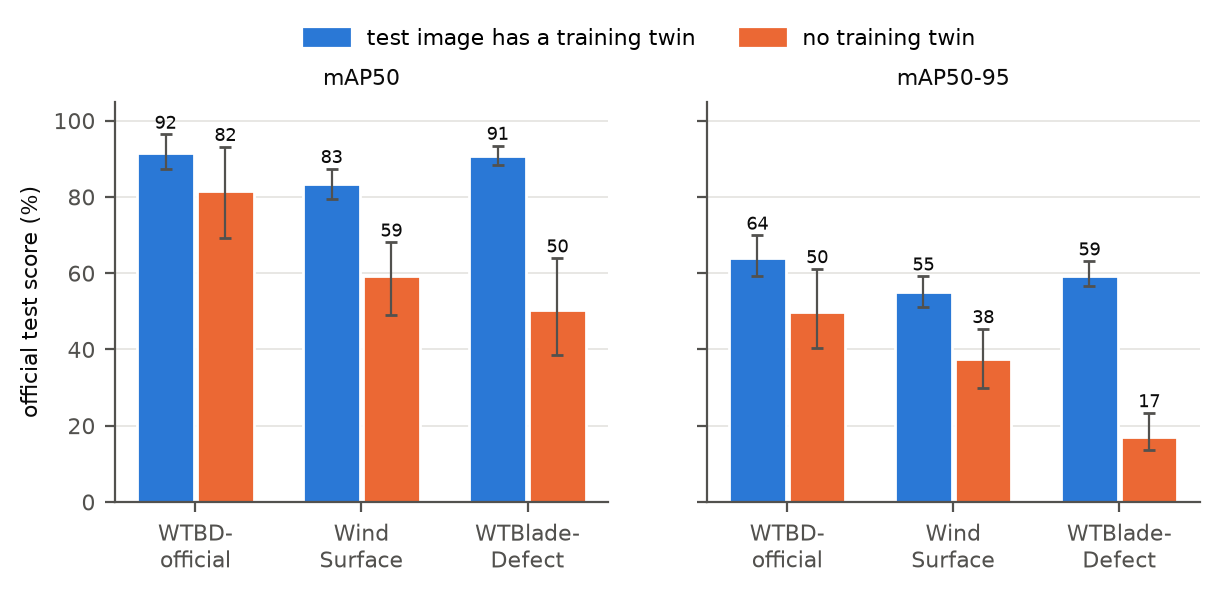
\includegraphics[width=0.88\linewidth,height=\textheight,keepaspectratio,alt={Figure 6. Official-protocol scores of the best RF-DETR-M run on leaked and no-twin test images. Bars show the COCO-style evaluator with image-bootstrap 95\% intervals.}]{figures/fig1_leak_subsets.png}
\caption{Figure 6. Official-protocol scores of the best RF-DETR-M run on
leaked and no-twin test images. Bars show the COCO-style evaluator with
image-bootstrap 95\% intervals.}
\end{figure}

WTBlade-Defect's official number is mostly its copies: 98.2 on copies of
training frames and 50.4 with no same-scene training image. The
independently built WTBlade-group benchmark agrees from a different
direction: its RF-DETR-M runs score 16.1--17.3 mAP50-95 (Table~7)
against 17.2 here. Their 38.5--41.8 mAP50 is inside this small subset's
interval of {[}38.5, 64.0{]}.

WTBD's no-twin subset is too small to read on its own: it holds a single
box each of craze, thunderstrike and crack. Corrosion is the only class
with a clear drop (AP50 97 to 54). The split comparison below is
therefore the stronger evidence for WTBD.

\subsection{Same detector, only the split
differs}\label{same-detector-only-the-split-differs}

Table~4 and Fig.~7 compare models trained on the same 1,065 WTBD images,
official against scene-grouped.

\begin{longtable}[]{@{}
  >{\raggedright\arraybackslash}p{(\linewidth - 12\tabcolsep) * \real{0.1429}}
  >{\raggedright\arraybackslash}p{(\linewidth - 12\tabcolsep) * \real{0.1429}}
  >{\raggedright\arraybackslash}p{(\linewidth - 12\tabcolsep) * \real{0.1429}}
  >{\raggedright\arraybackslash}p{(\linewidth - 12\tabcolsep) * \real{0.1429}}
  >{\raggedright\arraybackslash}p{(\linewidth - 12\tabcolsep) * \real{0.1429}}
  >{\raggedright\arraybackslash}p{(\linewidth - 12\tabcolsep) * \real{0.1429}}
  >{\raggedright\arraybackslash}p{(\linewidth - 12\tabcolsep) * \real{0.1429}}@{}}
\caption{Table 4. Same recipe, only the WTBD split differs. Test AP50 by
class and overall mAP50 / mAP50-95. BladeYOLO-v2 and YOLO12-L use
Ultralytics \texttt{val} and trained for 120 epochs on the official
split and 150 on the group split. RF-DETR-M uses the COCO-style
evaluator (seed 0), 768 px and 100 epochs on both splits, with an
effective batch of 16 on both (2 × 8 and 4 × 4).}\tabularnewline
\toprule\noalign{}
\begin{minipage}[b]{\linewidth}\raggedright
class
\end{minipage} & \begin{minipage}[b]{\linewidth}\raggedright
BladeYOLO-v2 official
\end{minipage} & \begin{minipage}[b]{\linewidth}\raggedright
BladeYOLO-v2 group
\end{minipage} & \begin{minipage}[b]{\linewidth}\raggedright
YOLO12-L official
\end{minipage} & \begin{minipage}[b]{\linewidth}\raggedright
YOLO12-L group
\end{minipage} & \begin{minipage}[b]{\linewidth}\raggedright
RF-DETR-M official
\end{minipage} & \begin{minipage}[b]{\linewidth}\raggedright
RF-DETR-M group
\end{minipage} \\
\midrule\noalign{}
\endfirsthead
\toprule\noalign{}
\begin{minipage}[b]{\linewidth}\raggedright
class
\end{minipage} & \begin{minipage}[b]{\linewidth}\raggedright
BladeYOLO-v2 official
\end{minipage} & \begin{minipage}[b]{\linewidth}\raggedright
BladeYOLO-v2 group
\end{minipage} & \begin{minipage}[b]{\linewidth}\raggedright
YOLO12-L official
\end{minipage} & \begin{minipage}[b]{\linewidth}\raggedright
YOLO12-L group
\end{minipage} & \begin{minipage}[b]{\linewidth}\raggedright
RF-DETR-M official
\end{minipage} & \begin{minipage}[b]{\linewidth}\raggedright
RF-DETR-M group
\end{minipage} \\
\midrule\noalign{}
\endhead
\bottomrule\noalign{}
\endlastfoot
crack & 99.1 & 38.1 & 85.4 & 38.4 & 95.3 & 61 \\
craze & 90.9 & 7.6 & 62.2 & 6.5 & 95.3 & 9 \\
hide\_craze & 80.0 & 56.9 & 63.9 & 52.6 & 80.3 & 71 \\
surface\_injure & 81.6 & 74.7 & 71.1 & 62.9 & 91.0 & 83 \\
thunderstrike & 99.5 & 98.0 & 93.8 & 41.8 & 94.3 & 64 \\
corrosion & 52.7 & 53.8 & 46.0 & 60.8 & 86.0 & 46 \\
\textbf{all} & \textbf{84.0 / 49.3} & \textbf{54.8 / 24.5} &
\textbf{70.4 / 38.8} & \textbf{43.8 / 20.6} & \textbf{90.4 / 61.2} &
\textbf{55.3 / 33.2} \\
\end{longtable}

\begin{figure}
\centering
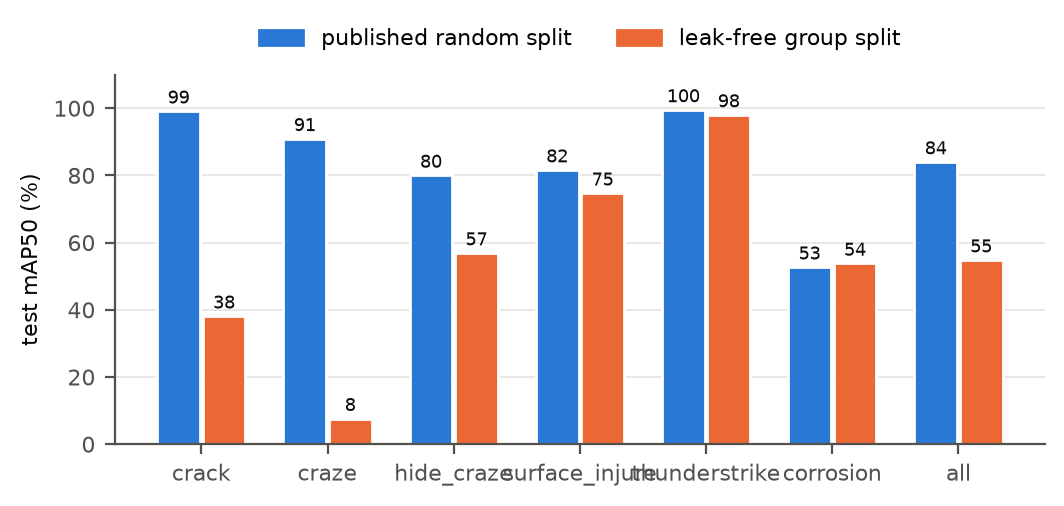
\includegraphics[width=0.78\linewidth,height=\textheight,keepaspectratio,alt={Figure 7. Inflation per class on WTBD for BladeYOLO-v2 and YOLO12-L, from the same recipe on the official and the group split.}]{figures/fig3_wtbd_inflation.png}
\caption{Figure 7. Inflation per class on WTBD for BladeYOLO-v2 and
YOLO12-L, from the same recipe on the official and the group split.}
\end{figure}

The inflation is model-independent: +29.2 mAP50 for BladeYOLO-v2, +26.6
for YOLO12-L and +35.1 for RF-DETR-M, with mAP50-95 multiplied by 2.0,
1.9 and 1.8. Fig.~10 (c) adds WTBlade: 87.2 / 55.1 officially and 38.5 /
16.2 on WTBlade-group. That second pair is not a pure split comparison,
because WTBlade-group also keeps one frame per source and 60 rather than
40 epochs.

\subsection{Tuning on the official splits rewards
memorisation}\label{tuning-on-the-official-splits-rewards-memorisation}

Between G25 and G26 we made one tuning step in the usual spirit, moving
to a cosine schedule (and on two protocols, longer training) because the
official numbers improved. Table~5 decomposes what that step bought
(post hoc).

\begin{longtable}[]{@{}
  >{\raggedright\arraybackslash}p{(\linewidth - 8\tabcolsep) * \real{0.2000}}
  >{\raggedright\arraybackslash}p{(\linewidth - 8\tabcolsep) * \real{0.2000}}
  >{\raggedright\arraybackslash}p{(\linewidth - 8\tabcolsep) * \real{0.2000}}
  >{\raggedright\arraybackslash}p{(\linewidth - 8\tabcolsep) * \real{0.2000}}
  >{\raggedright\arraybackslash}p{(\linewidth - 8\tabcolsep) * \real{0.2000}}@{}}
\caption{Table 5. What one tuning step bought. Paired image bootstrap, Δ
mAP50-95 in points = G26 recipe − G25 recipe, same images. Interaction =
Δ leaked − Δ no twin, with the subsets resampled
independently.}\tabularnewline
\toprule\noalign{}
\begin{minipage}[b]{\linewidth}\raggedright
protocol (change)
\end{minipage} & \begin{minipage}[b]{\linewidth}\raggedright
Δ all
\end{minipage} & \begin{minipage}[b]{\linewidth}\raggedright
Δ leaked
\end{minipage} & \begin{minipage}[b]{\linewidth}\raggedright
Δ no twin
\end{minipage} & \begin{minipage}[b]{\linewidth}\raggedright
interaction, P(\textgreater0)
\end{minipage} \\
\midrule\noalign{}
\endfirsthead
\toprule\noalign{}
\begin{minipage}[b]{\linewidth}\raggedright
protocol (change)
\end{minipage} & \begin{minipage}[b]{\linewidth}\raggedright
Δ all
\end{minipage} & \begin{minipage}[b]{\linewidth}\raggedright
Δ leaked
\end{minipage} & \begin{minipage}[b]{\linewidth}\raggedright
Δ no twin
\end{minipage} & \begin{minipage}[b]{\linewidth}\raggedright
interaction, P(\textgreater0)
\end{minipage} \\
\midrule\noalign{}
\endhead
\bottomrule\noalign{}
\endlastfoot
WTBD-official (constant → cosine) & +1.0 {[}−1.2, +3.0{]} & +1.8
{[}−0.1, +4.0{]} & −8.1 {[}−13.4, +0.2{]} & +9.9 {[}+1.1, +15.8{]},
0.993 \\
Wind Surface (60 ep constant → 100 ep cosine) & +1.8 {[}+0.5, +3.1{]} &
+2.3 {[}+0.9, +3.8{]} & −1.5 {[}−4.2, +1.4{]} & +3.8 {[}+0.7, +7.0{]},
0.988 \\
WTBlade-Defect (25 ep constant → 40 ep cosine) & +2.6 {[}+1.1, +3.9{]} &
+3.5 {[}+2.0, +5.0{]}; copies +5.4 {[}+3.6, +7.0{]} & −4.0 {[}−7.2,
+0.1{]} & +7.4 {[}+3.0, +11.1{]}, 1.000 \\
\end{longtable}

\begin{figure}
\centering
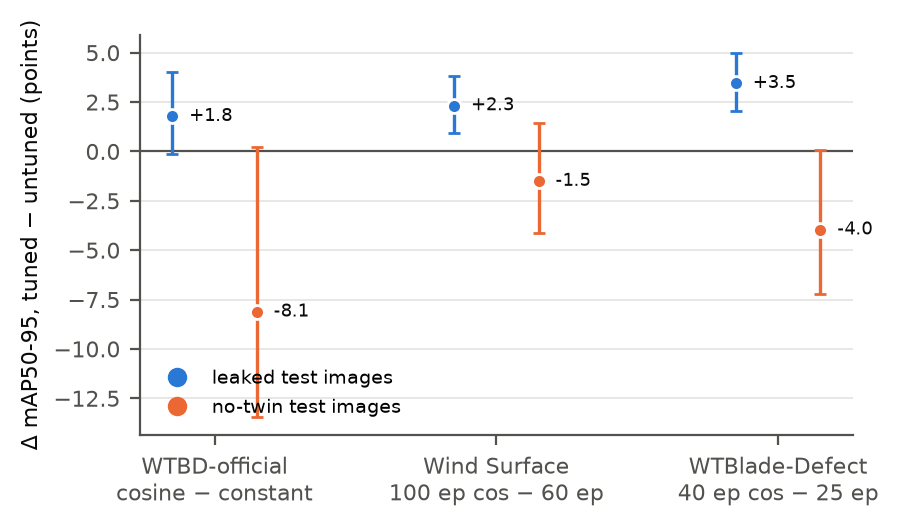
\includegraphics[width=0.84\linewidth,height=\textheight,keepaspectratio,alt={Figure 8. The tuning step of Table~5: gains sit on leaked images, and the same change lowers the no-twin score.}]{figures/fig2_tuning_memorisation.png}
\caption{Figure 8. The tuning step of Table~5: gains sit on leaked
images, and the same change lowers the no-twin score.}
\end{figure}

On every protocol the gain sits on leaked images, and the same change
lowers the score on images without a twin. At mAP50 the change is −0.2
to −0.8 overall and −5.0 to −6.0 on no-twin images. The interaction
excludes zero on all three. This applies to our own G26 numbers, which
stay in Table~2 labelled as what they are. Two confounds remain: on Wind
Surface and WTBlade-Defect the epoch count also changed (on WTBD only
the schedule changed, with the same pattern), and this is one tuning
step, not a study of tuning in general.

A second reading comes from the leaderboard itself. RF-DETR-M leads
BladeYOLO-v2 on WTBD-official by +13.2 {[}+8.2, +17.4{]} mAP50-95 on all
images, but by only +2.1 {[}−5.3, +19.8{]} on the 36 no-twin images, so
that official lead is not established on unseen images.

\subsection{Consequence for deployment: leaked calibration breaks recall
guarantees}\label{consequence-for-deployment-leaked-calibration-breaks-recall-guarantees}

An inspection system should promise a bound on missed defects. Conformal
risk control {[}\citeproc{ref-crc}{27}{]} picks a confidence threshold
so that the expected share of missed defects is at most α. A defect
counts as flagged if at least 50\% of its box is covered by predictions
above the threshold. We calibrate on seen or unseen scenes and always
deploy on unseen scenes (Table~6, Fig.~9).

\begin{longtable}[]{@{}
  >{\raggedright\arraybackslash}p{(\linewidth - 6\tabcolsep) * \real{0.2500}}
  >{\raggedright\arraybackslash}p{(\linewidth - 6\tabcolsep) * \real{0.2500}}
  >{\raggedright\arraybackslash}p{(\linewidth - 6\tabcolsep) * \real{0.2500}}
  >{\raggedright\arraybackslash}p{(\linewidth - 6\tabcolsep) * \real{0.2500}}@{}}
\caption{Table 6. Conformal recall guarantee, target ≤ 10\% missed
(BladeYOLO-v2, 500 draws of 100 calibration images, or scene groups as
units).}\tabularnewline
\toprule\noalign{}
\begin{minipage}[b]{\linewidth}\raggedright
calibrated on
\end{minipage} & \begin{minipage}[b]{\linewidth}\raggedright
deployed on
\end{minipage} & \begin{minipage}[b]{\linewidth}\raggedright
realised miss rate
\end{minipage} & \begin{minipage}[b]{\linewidth}\raggedright
draws violating
\end{minipage} \\
\midrule\noalign{}
\endfirsthead
\toprule\noalign{}
\begin{minipage}[b]{\linewidth}\raggedright
calibrated on
\end{minipage} & \begin{minipage}[b]{\linewidth}\raggedright
deployed on
\end{minipage} & \begin{minipage}[b]{\linewidth}\raggedright
realised miss rate
\end{minipage} & \begin{minipage}[b]{\linewidth}\raggedright
draws violating
\end{minipage} \\
\midrule\noalign{}
\endhead
\bottomrule\noalign{}
\endlastfoot
seen scenes (group train), image units & unseen scenes & \textbf{31.5\%}
& 100\% \\
seen scenes, scene units & unseen scenes & 28.8\% & 100\% \\
unseen scenes (group val), image units & unseen scenes & 6.3\% & 0\% \\
unseen scenes, scene units & unseen scenes & 4.7\% & 1\% \\
official val (leaky) & official test, images with a twin & 12.6\% &
91\% \\
official val (leaky) & official test, no-twin images & \textbf{25.9\%} &
100\% \\
\end{longtable}

\begin{figure}
\centering
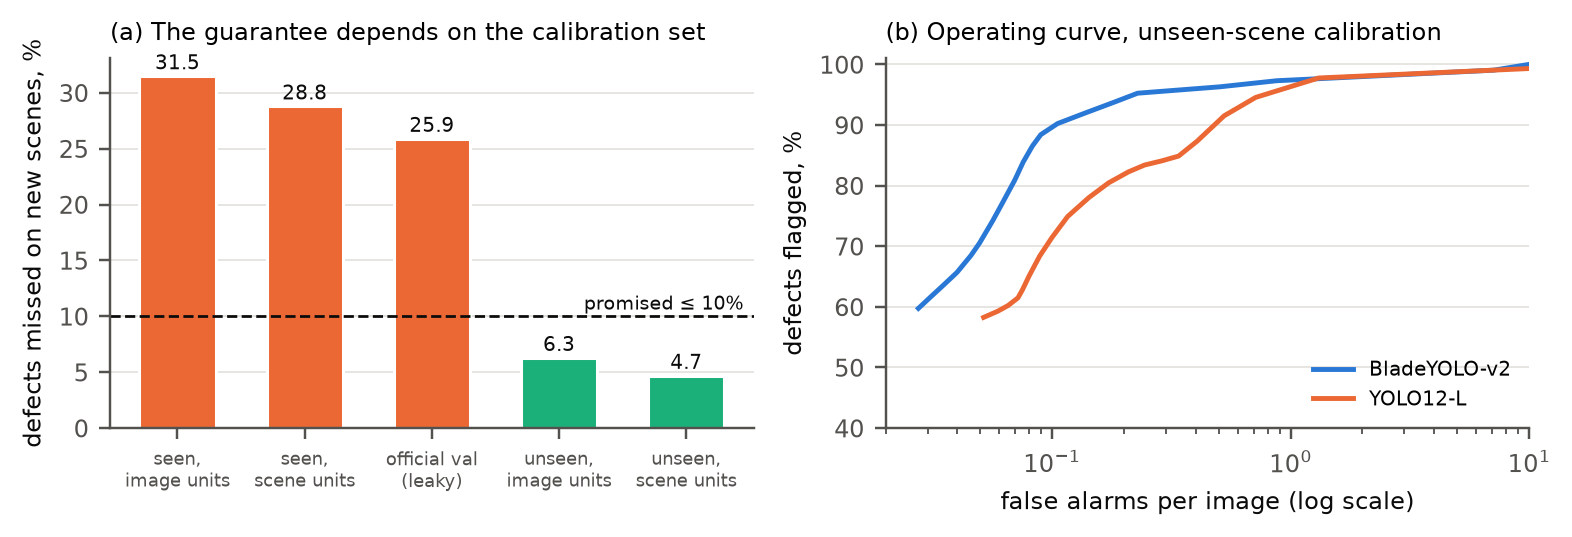
\includegraphics[width=0.92\linewidth,height=\textheight,keepaspectratio,alt={Figure 9. (a) Realised miss rate on new scenes, by calibration set. (b) Operating curve with scene units, calibrated on unseen scenes. At 0.1 false alarms per image BladeYOLO-v2 flags about 90\% of defects on new scenes, YOLO12-L about 71\%. One test set of 58 scenes; the curve has no interval.}]{figures/fig14_conformal.png}
\caption{Figure 9. (a) Realised miss rate on new scenes, by calibration
set. (b) Operating curve with scene units, calibrated on unseen scenes.
At 0.1 false alarms per image BladeYOLO-v2 flags about 90\% of defects
on new scenes, YOLO12-L about 71\%. One test set of 58 scenes; the curve
has no interval.}
\end{figure}

Models are overconfident on what they memorised, so a threshold
calibrated on seen scenes is too high for new data. The practical rule
is that calibration data must be split by scene, as test data must. The
honest calibration is cheap: 0.2 instead of 0.1 false alarms per image.
With only 60 calibration and 58 deployment scenes from one site, the val
and test groups are not perfectly exchangeable: YOLO12-L still misses
12.3\% with scene-unit calibration on unseen scenes, violated in 71\% of
draws.

\section{Leak-free results: what helps}\label{sec:leakfree}

\subsection{The benchmark at full
labels}\label{the-benchmark-at-full-labels}

Table~7, Fig.~10 and Fig.~11 give the benchmark, all with one evaluator.

\begin{longtable}[]{@{}
  >{\raggedright\arraybackslash}p{(\linewidth - 4\tabcolsep) * \real{0.3333}}
  >{\raggedright\arraybackslash}p{(\linewidth - 4\tabcolsep) * \real{0.3333}}
  >{\raggedright\arraybackslash}p{(\linewidth - 4\tabcolsep) * \real{0.3333}}@{}}
\caption{Table 7. Leak-free benchmark, full labels, test mAP50 /
mAP50-95, COCO-style evaluator on cached predictions. YOLO12-L on
WTBlade-group trained for 50 epochs, reached its best validation at
epoch 43, and rose almost linearly until then (Fig.~15 f), so its row
may understate it. No paired interval was computed for the
cross-architecture comparisons in this table, so treat them as point
estimates.}\tabularnewline
\toprule\noalign{}
\begin{minipage}[b]{\linewidth}\raggedright
model
\end{minipage} & \begin{minipage}[b]{\linewidth}\raggedright
WTBD-group (161 images, 58 scenes)
\end{minipage} & \begin{minipage}[b]{\linewidth}\raggedright
WTBlade-group (332 frames, 177 scenes)
\end{minipage} \\
\midrule\noalign{}
\endfirsthead
\toprule\noalign{}
\begin{minipage}[b]{\linewidth}\raggedright
model
\end{minipage} & \begin{minipage}[b]{\linewidth}\raggedright
WTBD-group (161 images, 58 scenes)
\end{minipage} & \begin{minipage}[b]{\linewidth}\raggedright
WTBlade-group (332 frames, 177 scenes)
\end{minipage} \\
\midrule\noalign{}
\endhead
\bottomrule\noalign{}
\endlastfoot
YOLO12-L & 40.0 / 18.5 & 32.2 / 13.3 \\
BladeYOLO-v2 without DINOv3 & 31.8 / 15.2 & not run \\
BladeYOLO-v2 & 56.1 / 24.4 (ViT-S) & 41.8 / 18.0 (ViT-B) \\
RF-DETR-M, A0, seeds 0 / 1 & 55.3 / 33.2, 54.8 / 32.2 & 38.5 / 16.2,
41.0 / 16.9 \\
RF-DETR-M + copy-paste, A1, seeds 0 / 1 & 51.5 / 30.7, 58.5 / 32.7 &
41.8 / 17.3, 39.3 / 16.5 \\
RF-DETR-M + copy-paste + in-domain SSL, A2 & 49.6 / 27.4 & 40.1 /
16.1 \\
RF-DETR-M + copy-paste + multi-dataset stage 1, A3 & 55.3 / 33.2 & 41.7
/ 16.6 \\
\end{longtable}

\begin{figure}
\centering
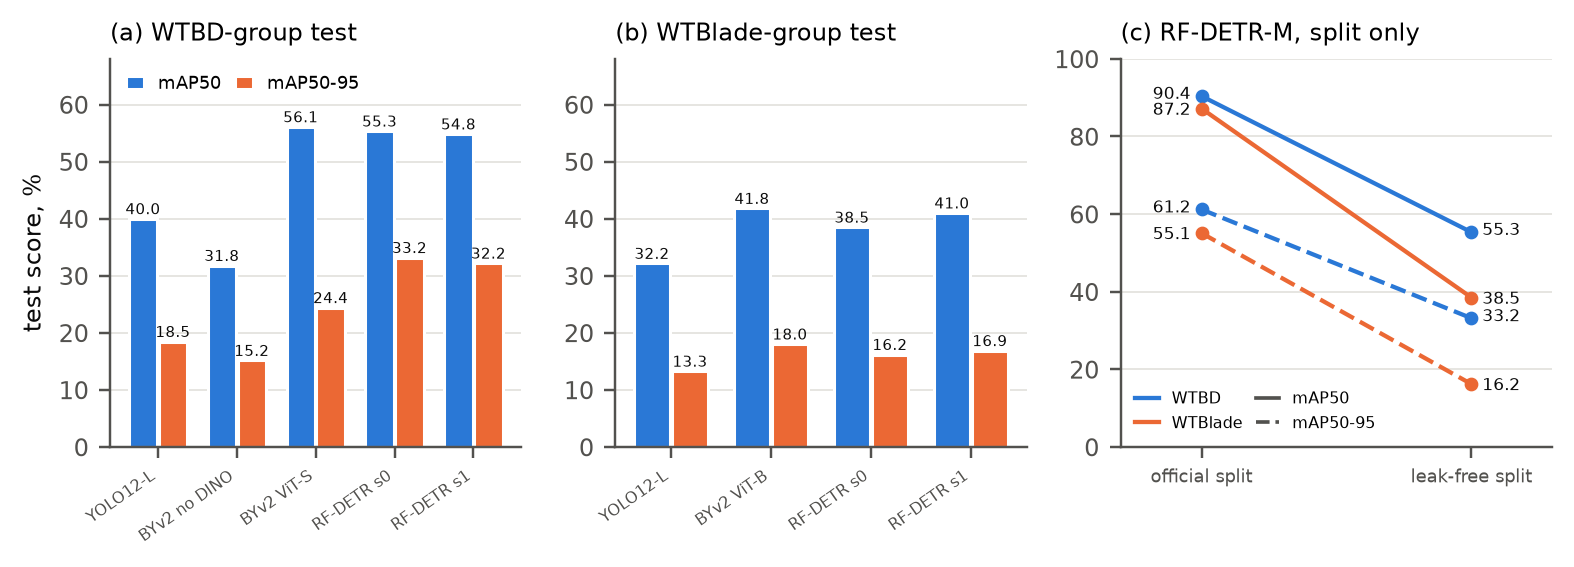
\includegraphics[width=1\linewidth,height=\textheight,keepaspectratio,alt={Figure 10. (a, b) Leak-free test scores by model (BYv2: BladeYOLO-v2; s0, s1: seeds). (c) RF-DETR-M on official and leak-free splits.}]{figures/fig17_benchmark.png}
\caption{Figure 10. (a, b) Leak-free test scores by model (BYv2:
BladeYOLO-v2; s0, s1: seeds). (c) RF-DETR-M on official and leak-free
splits.}
\end{figure}

\begin{figure}
\centering
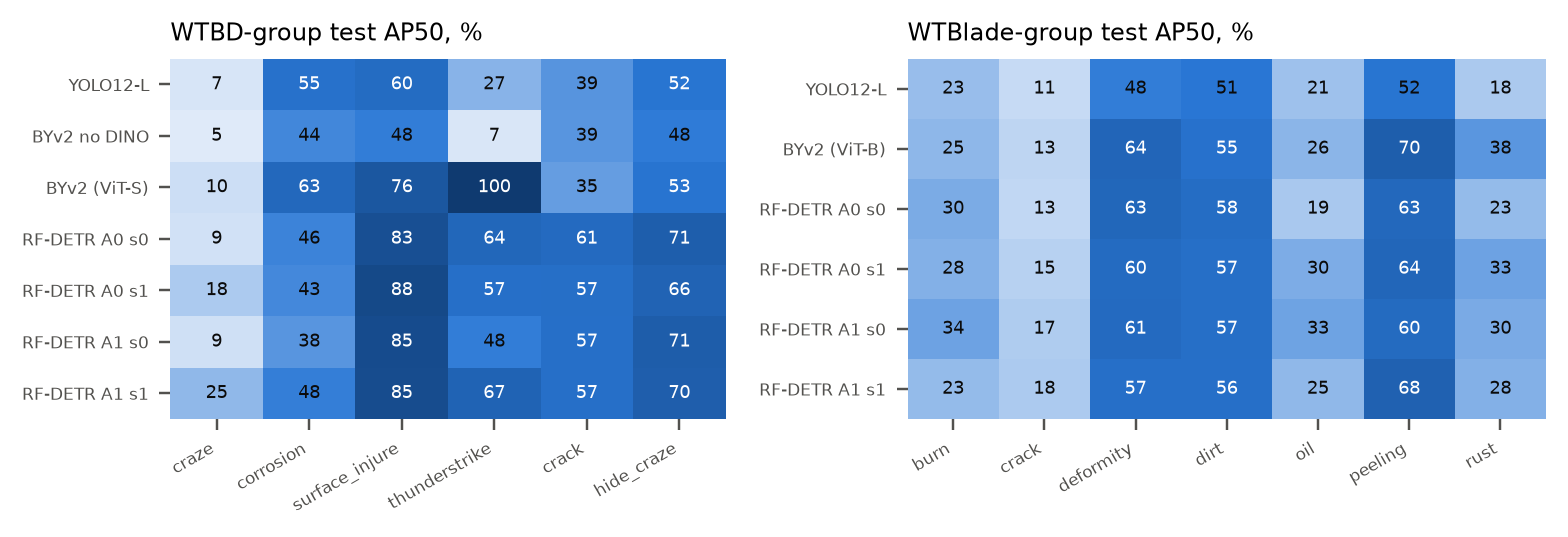
\includegraphics[width=0.98\linewidth,height=\textheight,keepaspectratio,alt={Figure 11. Per-class test AP50 on the leak-free benchmarks. Note the seed-to-seed swings within RF-DETR on rare classes (craze 9--25, thunderstrike 48--67), and BladeYOLO-v2's thunderstrike 100, which rests on 3 test scenes.}]{figures/fig24_per_class.png}
\caption{Figure 11. Per-class test AP50 on the leak-free benchmarks.
Note the seed-to-seed swings within RF-DETR on rare classes (craze
9--25, thunderstrike 48--67), and BladeYOLO-v2's thunderstrike 100,
which rests on 3 test scenes.}
\end{figure}

Four points stand out:

\begin{itemize}
\tightlist
\item
  \textbf{The ranking depends on the dataset.} RF-DETR-M leads on
  WTBD-group by 8--9 mAP50-95 points over BladeYOLO-v2, but on
  WTBlade-group the frozen ViT-B BladeYOLO-v2 (18.0) is ahead of every
  RF-DETR run (16.1--17.3). A ``generic detector is strongest'' claim
  holds on one benchmark.
\item
  \textbf{On WTBD the RF-DETR gain is box quality, not finding.} mAP50
  is level with BladeYOLO-v2 (55.3 and 54.8 against 56.1) while mAP50-95
  is 8--9 points higher. This matches the extent analysis in §~7.
\item
  \textbf{Classification costs points on RF-DETR.} Scoring A0 with
  classes merged gives 66.1 / 40.5 on WTBD-group and 50.1 / 21.3 on
  WTBlade-group (Table~15), about 11 AP50 points above its class-aware
  score. BladeYOLO-v2's class-agnostic and class-aware AP50 are about
  equal (56.3 against 56.1), while YOLO12-L shows a gap like RF-DETR's
  (48.5 against 40.0).
\item
  \textbf{The earlier BladeYOLO-v2 win over YOLO12-L rests largely on
  thunderstrike.} The scene bootstrap gives +16.1 {[}+2.5, +28.4{]}
  mAP50 and +5.9 {[}+0.5, +16.9{]} mAP50-95, but without the two classes
  seen in at most 3 test scenes the mAP50 gain is +5.2 {[}−2.7,
  +13.5{]}.
\end{itemize}

\subsection{Where the advantage comes from: DINOv3
ablation}\label{where-the-advantage-comes-from-dinov3-ablation}

We removed only the frozen DINOv3 features from BladeYOLO-v2, keeping
deformable refinement, selective scan and WIoU, at 25\%, 50\% and 100\%
of the labelled scenes (Table~8, Fig.~12).

\begin{longtable}[]{@{}
  >{\raggedright\arraybackslash}p{(\linewidth - 6\tabcolsep) * \real{0.2500}}
  >{\raggedright\arraybackslash}p{(\linewidth - 6\tabcolsep) * \real{0.2500}}
  >{\raggedright\arraybackslash}p{(\linewidth - 6\tabcolsep) * \real{0.2500}}
  >{\raggedright\arraybackslash}p{(\linewidth - 6\tabcolsep) * \real{0.2500}}@{}}
\caption{Table 8. DINOv3 ablation and learning curve, WTBD-group, test
mAP50-95, scene bootstrap. Last row: stock YOLO12-L compared with our
modules without DINOv3.}\tabularnewline
\toprule\noalign{}
\begin{minipage}[b]{\linewidth}\raggedright
\end{minipage} & \begin{minipage}[b]{\linewidth}\raggedright
25\%
\end{minipage} & \begin{minipage}[b]{\linewidth}\raggedright
50\%
\end{minipage} & \begin{minipage}[b]{\linewidth}\raggedright
100\%
\end{minipage} \\
\midrule\noalign{}
\endfirsthead
\toprule\noalign{}
\begin{minipage}[b]{\linewidth}\raggedright
\end{minipage} & \begin{minipage}[b]{\linewidth}\raggedright
25\%
\end{minipage} & \begin{minipage}[b]{\linewidth}\raggedright
50\%
\end{minipage} & \begin{minipage}[b]{\linewidth}\raggedright
100\%
\end{minipage} \\
\midrule\noalign{}
\endhead
\bottomrule\noalign{}
\endlastfoot
BladeYOLO-v2 (frozen DINOv3 ViT-S) & 7.6 (3 seeds) & 17.5 & 24.2 (2
seeds) \\
without DINOv3 & 3.7 (2 seeds) & 8.8 & 15.2 \\
YOLO12-L (stock) & 4.1 & 9.9 & 18.5 \\
\textbf{DINOv3 gain} & \textbf{+3.9 {[}+2.5, +10.1{]}} & \textbf{+8.8
{[}+4.0, +22.1{]}} & \textbf{+9.0 {[}+4.0, +20.5{]}} \\
same, 4 well-represented classes & +4.4 {[}+2.3, +11.1{]} & +6.1
{[}+2.2, +17.9{]} & +4.9 {[}−1.8, +10.3{]} \\
YOLO12-L − without DINOv3 & +0.4 & +1.1 & +3.3 {[}−0.2, +13.1{]} \\
\end{longtable}

\begin{figure}
\centering
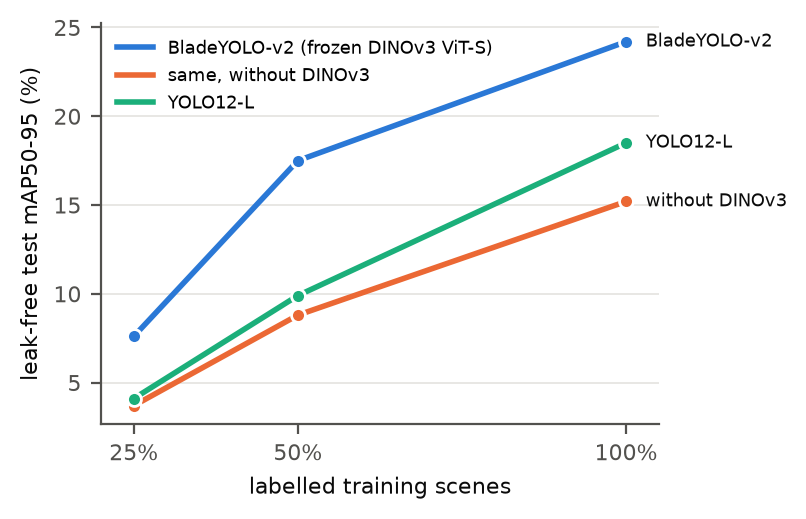
\includegraphics[width=0.74\linewidth,height=\textheight,keepaspectratio,alt={Figure 12. Learning curves with and without frozen DINOv3 on WTBD-group. The modules around DINOv3 do not put the model above stock YOLO12-L.}]{figures/fig4_dinov3_learning_curve.png}
\caption{Figure 12. Learning curves with and without frozen DINOv3 on
WTBD-group. The modules around DINOv3 do not put the model above stock
YOLO12-L.}
\end{figure}

Without DINOv3, BladeYOLO-v2 equals or trails stock YOLO12-L at every
data size. The advantage is therefore the features, not the architecture
around them. We first read it as a low-data advantage; the 50\% and
100\% runs corrected that, since the absolute gain does not shrink with
data. Only the relative gain does (2.0× to 1.6×). This claim concerns
our components. BladeYOLO's exact Style Injection, WTConv and
Cross-Mamba modules were reimplemented only before our code audit
(§~10), so we make no claim about them.

\textbf{Backbone size at 25\%} (Table~9). A larger frozen backbone helps
up to ViT-B, and ViT-L adds nothing further.

\begin{longtable}[]{@{}
  >{\raggedright\arraybackslash}p{(\linewidth - 6\tabcolsep) * \real{0.2500}}
  >{\raggedright\arraybackslash}p{(\linewidth - 6\tabcolsep) * \real{0.2500}}
  >{\raggedright\arraybackslash}p{(\linewidth - 6\tabcolsep) * \real{0.2500}}
  >{\raggedright\arraybackslash}p{(\linewidth - 6\tabcolsep) * \real{0.2500}}@{}}
\caption{Table 9. Frozen DINOv3 size at 25\% of WTBD-group scenes. Test
scores by Ultralytics \texttt{val}; differences by scene bootstrap,
mAP50-95 in points.}\tabularnewline
\toprule\noalign{}
\begin{minipage}[b]{\linewidth}\raggedright
backbone
\end{minipage} & \begin{minipage}[b]{\linewidth}\raggedright
test mAP50 / mAP50-95 per seed
\end{minipage} & \begin{minipage}[b]{\linewidth}\raggedright
difference
\end{minipage} & \begin{minipage}[b]{\linewidth}\raggedright
Δ mAP50-95 {[}95\% CI{]}
\end{minipage} \\
\midrule\noalign{}
\endfirsthead
\toprule\noalign{}
\begin{minipage}[b]{\linewidth}\raggedright
backbone
\end{minipage} & \begin{minipage}[b]{\linewidth}\raggedright
test mAP50 / mAP50-95 per seed
\end{minipage} & \begin{minipage}[b]{\linewidth}\raggedright
difference
\end{minipage} & \begin{minipage}[b]{\linewidth}\raggedright
Δ mAP50-95 {[}95\% CI{]}
\end{minipage} \\
\midrule\noalign{}
\endhead
\bottomrule\noalign{}
\endlastfoot
ViT-S/16, 3 seeds & 23.2 / 8.2, 22.4 / 8.7, 18.4 / 6.8 & & \\
ViT-B/16, 2 seeds & 25.2 / 10.2, 28.3 / 11.6 & ViT-B − ViT-S & +2.8
{[}+0.4, +9.6{]} \\
ViT-L/16, 2 seeds & 33.7 / 11.5, 30.1 / 10.9 & ViT-L − ViT-B & +0.3
{[}−4.0, +3.1{]} \\
without DINOv3, 2 seeds & 11.4 / 4.4, 8.1 / 3.1 & without − ViT-S & −3.9
{[}−10.1, −2.5{]} \\
\end{longtable}

\textbf{Fine-tuned against frozen foundation features, 25\% labels, same
subsets.} RF-DETR-M beats BladeYOLO-v2 ViT-B by +7.3 {[}+2.3, +11.9{]}
mAP50-95 (seed 0) and +8.3 {[}+4.5, +15.0{]} (seed 1), positive on 4 of
4 subsets at each seed. As a controlled comparison, freezing RF-DETR's
encoder lowers test mAP50-95 from 18.9 to 12.3 on WTBD and from 13.2 to
8.7 on WTBlade. Input resolution (G24) adds +1.0 from 576 to 768 on WTBD
(P 0.958) and −0.1 on WTBlade, whose frames are natively 640 px.

\subsection{Training behaviour}\label{training-behaviour}

Fig.~15 shows validation curves from every recent run. RF-DETR peaks
early and then drifts down, which is why EMA checkpoint selection
matters. In contrast, YOLO12-L on WTBlade-group rises almost linearly
until about epoch 43 of 50. Fig.~13 shows training and validation
batches, and Fig.~14 confusion matrices and a PR curve. In the matrices,
columns are true classes. The bottom row shows missed labels (crack 18\%
on WTBD-group and 27\% on WTBlade-group for YOLO12-L), the right column
shows where false positives go, and the strongest confusions involve
rare classes (YOLO12-L calls 54\% of thunderstrike labels craze on
WTBD-group test).

\begin{figure}
\centering
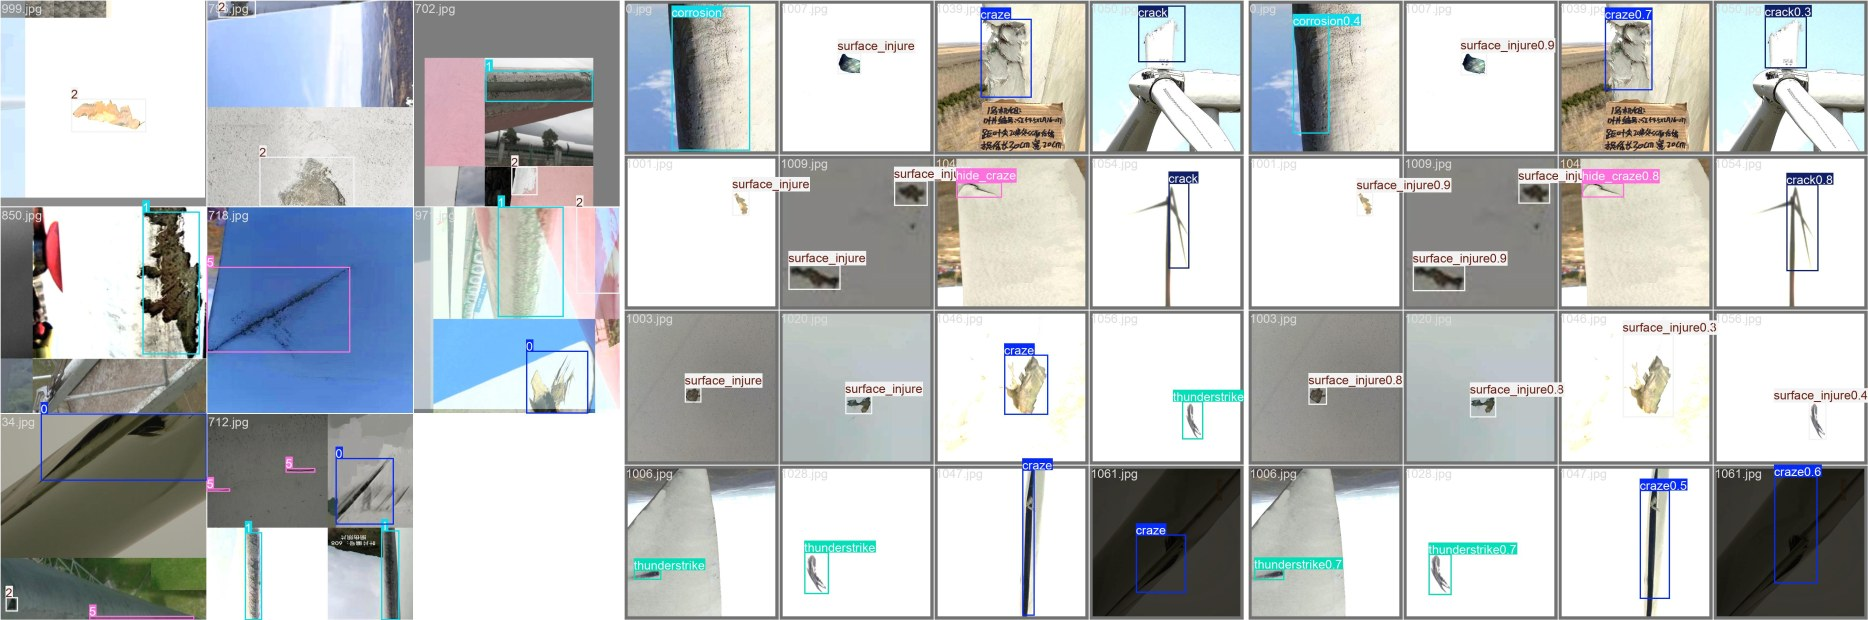
\includegraphics[width=1\linewidth,height=\textheight,keepaspectratio,alt={Figure 13. BladeYOLO-v2 on WTBD-group, from the training run. Left: a training batch after mosaic and flips. Middle: a validation batch with its labels. Right: the same batch with predictions.}]{figures/fig26_training_examples.jpg}
\caption{Figure 13. BladeYOLO-v2 on WTBD-group, from the training run.
Left: a training batch after mosaic and flips. Middle: a validation
batch with its labels. Right: the same batch with predictions.}
\end{figure}

\begin{figure}
\centering
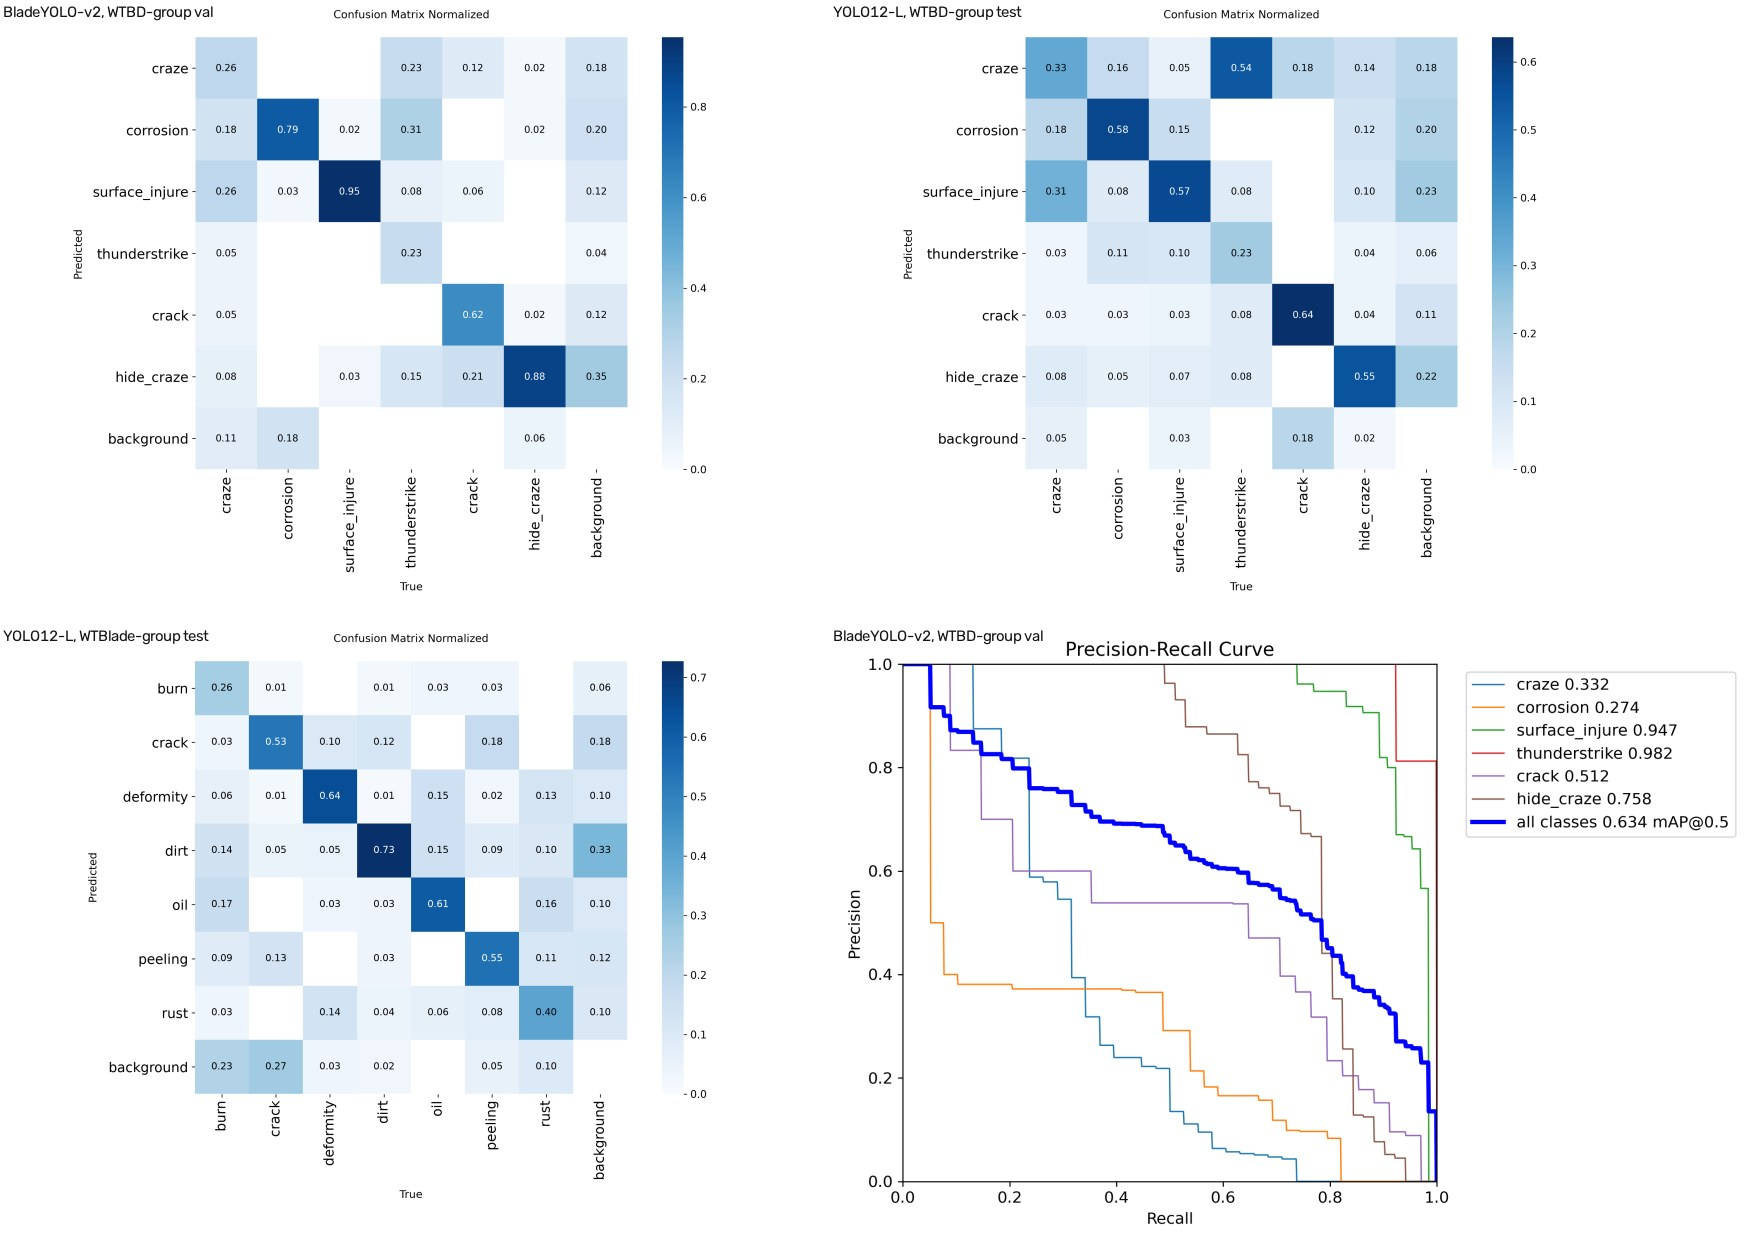
\includegraphics[width=0.84\linewidth,height=\textheight,keepaspectratio,alt={Figure 14. Diagnostics from the runs. Normalised confusion matrices: BladeYOLO-v2 on WTBD-group validation, YOLO12-L on WTBD-group test, and YOLO12-L on WTBlade-group test. Bottom right: PR curves by class of BladeYOLO-v2 on WTBD-group validation.}]{figures/fig27_diagnostics.jpg}
\caption{Figure 14. Diagnostics from the runs. Normalised confusion
matrices: BladeYOLO-v2 on WTBD-group validation, YOLO12-L on WTBD-group
test, and YOLO12-L on WTBlade-group test. Bottom right: PR curves by
class of BladeYOLO-v2 on WTBD-group validation.}
\end{figure}

\begin{figure}
\centering
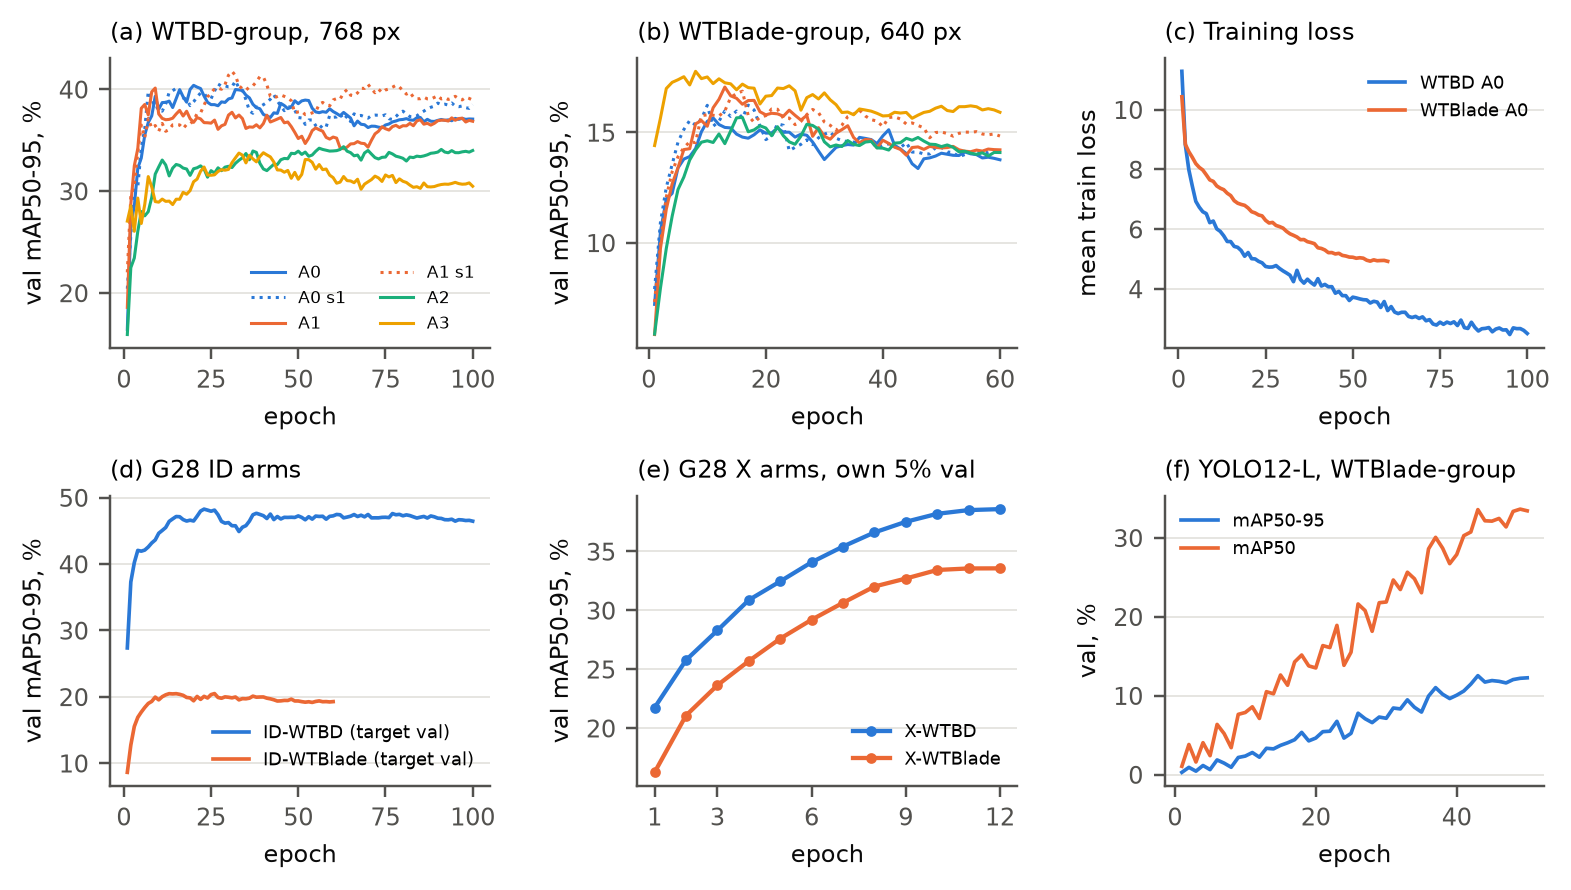
\includegraphics[width=1\linewidth,height=\textheight,keepaspectratio,alt={Figure 15. Training records. (a, b) Validation mAP50-95 of the G27 arms; dotted lines are seed 1. (c) Training loss of A0. (d) G28 ID arms on target validation. (e) G28 X arms on their own held-out 5\%, not comparable with (d) since the images differ. (f) YOLO12-L on WTBlade-group.}]{figures/fig15_training_curves.png}
\caption{Figure 15. Training records. (a, b) Validation mAP50-95 of the
G27 arms; dotted lines are seed 1. (c) Training loss of A0. (d) G28 ID
arms on target validation. (e) G28 X arms on their own held-out 5\%, not
comparable with (d) since the images differ. (f) YOLO12-L on
WTBlade-group.}
\end{figure}

\section{Why leak-free scores are low}\label{sec:why}

\subsection{The annotators against
themselves}\label{the-annotators-against-themselves}

WTBD's augmented copies were annotated independently, so aligned copies
of an image give accidental repeated labels. For every verified pair of
the same surface we project each label through the transform (flip-aware
ORB + RANSAC similarity, ≥ 25 inliers, at least 8 inliers inside the
box) and classify it as agree (same class, IoU ≥ 0.5), class conflict,
split, loose or missing. Fig.~16 shows examples and Table~10 gives the
rates.

\begin{figure}
\centering
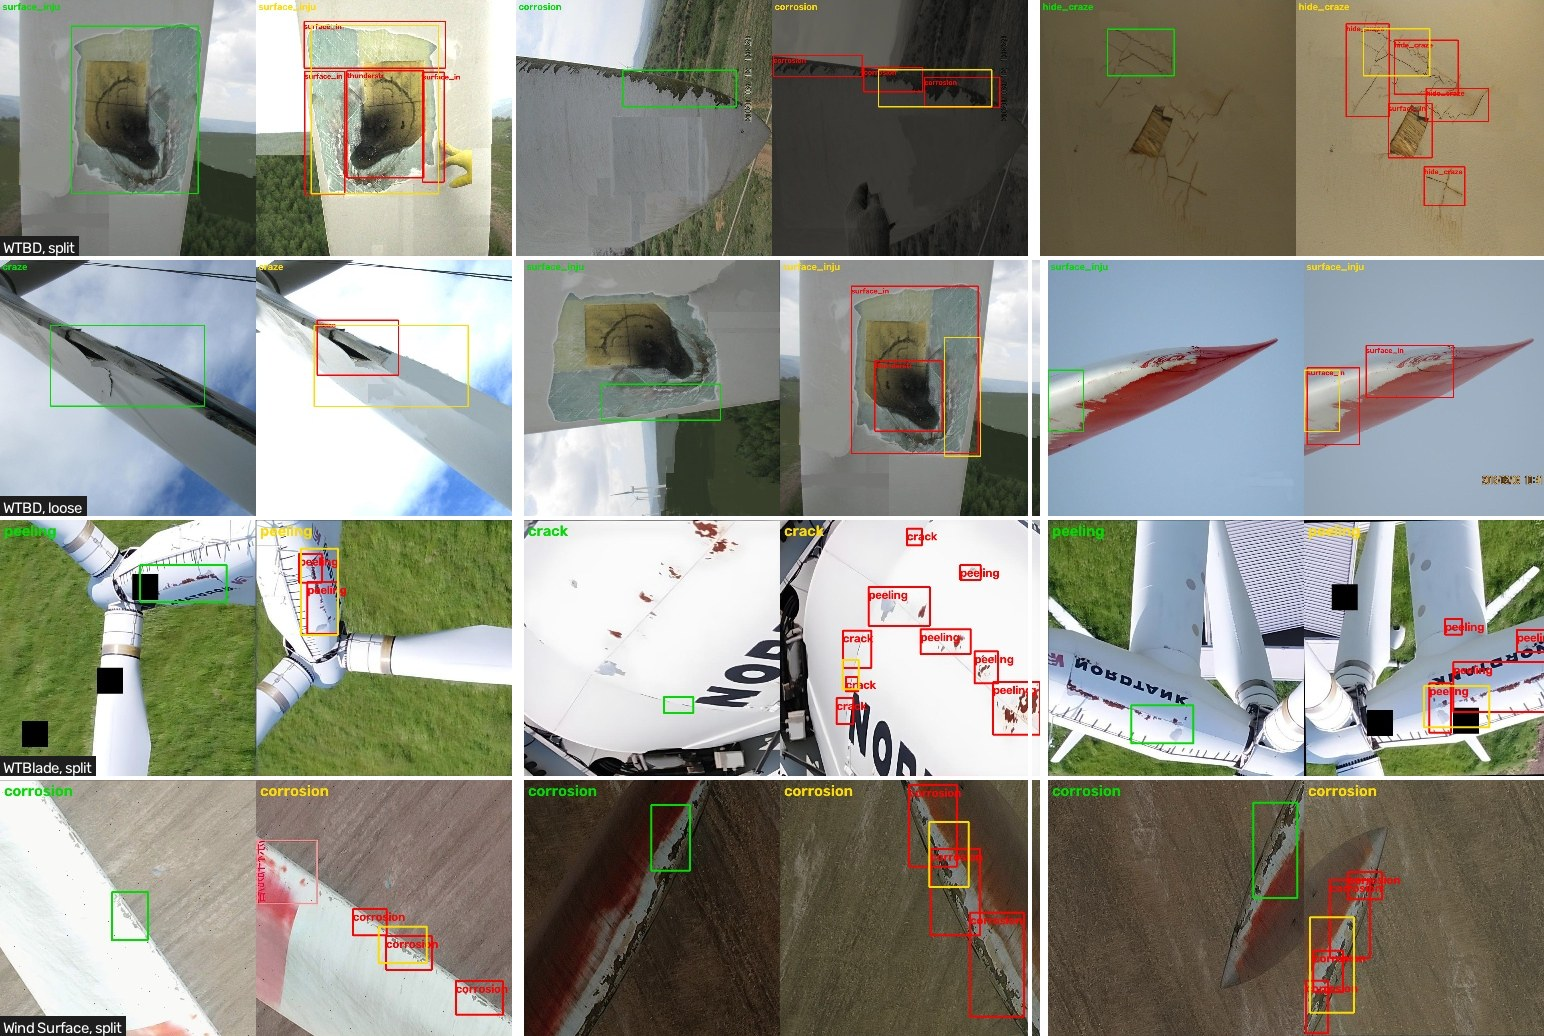
\includegraphics[width=0.92\linewidth,height=\textheight,keepaspectratio,alt={Figure 16. Annotation ambiguity on aligned copies. In each pair, left: a label (green). Right: its exact projection (yellow) and what the copy's annotator drew (red). Top two rows: WTBD. Third row: WTBlade-Defect. Bottom row: Wind Surface. The disagreement is about extent and how a defect is cut into boxes, not about the class. The pairs come from the audit's randomly ordered example sheets; ``NORDTANK'' is legible in the third row.}]{figures/fig11_label_ambiguity.jpg}
\caption{Figure 16. Annotation ambiguity on aligned copies. In each
pair, left: a label (green). Right: its exact projection (yellow) and
what the copy's annotator drew (red). Top two rows: WTBD. Third row:
WTBlade-Defect. Bottom row: Wind Surface. The disagreement is about
extent and how a defect is cut into boxes, not about the class. The
pairs come from the audit's randomly ordered example sheets;
``NORDTANK'' is legible in the third row.}
\end{figure}

\begin{longtable}[]{@{}
  >{\raggedright\arraybackslash}p{(\linewidth - 16\tabcolsep) * \real{0.1111}}
  >{\raggedright\arraybackslash}p{(\linewidth - 16\tabcolsep) * \real{0.1111}}
  >{\raggedright\arraybackslash}p{(\linewidth - 16\tabcolsep) * \real{0.1111}}
  >{\raggedright\arraybackslash}p{(\linewidth - 16\tabcolsep) * \real{0.1111}}
  >{\raggedright\arraybackslash}p{(\linewidth - 16\tabcolsep) * \real{0.1111}}
  >{\raggedright\arraybackslash}p{(\linewidth - 16\tabcolsep) * \real{0.1111}}
  >{\raggedright\arraybackslash}p{(\linewidth - 16\tabcolsep) * \real{0.1111}}
  >{\raggedright\arraybackslash}p{(\linewidth - 16\tabcolsep) * \real{0.1111}}
  >{\raggedright\arraybackslash}p{(\linewidth - 16\tabcolsep) * \real{0.1111}}@{}}
\caption{Table 10. Label self-consistency on axis-aligned copies of the
same image (rotation within 3° of a multiple of 90°, flips included),
where boxes map to boxes and every difference is an annotation
difference. Rotated copies and other views of the surface agree less,
but those strata also include geometric effects.}\tabularnewline
\toprule\noalign{}
\begin{minipage}[b]{\linewidth}\raggedright
dataset
\end{minipage} & \begin{minipage}[b]{\linewidth}\raggedright
labels
\end{minipage} & \begin{minipage}[b]{\linewidth}\raggedright
agree
\end{minipage} & \begin{minipage}[b]{\linewidth}\raggedright
split
\end{minipage} & \begin{minipage}[b]{\linewidth}\raggedright
loose
\end{minipage} & \begin{minipage}[b]{\linewidth}\raggedright
missing
\end{minipage} & \begin{minipage}[b]{\linewidth}\raggedright
class conflicts
\end{minipage} & \begin{minipage}[b]{\linewidth}\raggedright
rotated copies
\end{minipage} & \begin{minipage}[b]{\linewidth}\raggedright
other views
\end{minipage} \\
\midrule\noalign{}
\endfirsthead
\toprule\noalign{}
\begin{minipage}[b]{\linewidth}\raggedright
dataset
\end{minipage} & \begin{minipage}[b]{\linewidth}\raggedright
labels
\end{minipage} & \begin{minipage}[b]{\linewidth}\raggedright
agree
\end{minipage} & \begin{minipage}[b]{\linewidth}\raggedright
split
\end{minipage} & \begin{minipage}[b]{\linewidth}\raggedright
loose
\end{minipage} & \begin{minipage}[b]{\linewidth}\raggedright
missing
\end{minipage} & \begin{minipage}[b]{\linewidth}\raggedright
class conflicts
\end{minipage} & \begin{minipage}[b]{\linewidth}\raggedright
rotated copies
\end{minipage} & \begin{minipage}[b]{\linewidth}\raggedright
other views
\end{minipage} \\
\midrule\noalign{}
\endhead
\bottomrule\noalign{}
\endlastfoot
WTBD & 2,965 & \textbf{87.3\%} & 4.6\% & 6.7\% & 1.5\% & 0 & 77.9\% &
64.1\% \\
WTBlade-Defect & 42,812 & \textbf{86.0\%} & 2.5\% & 8.2\% & 3.1\% & 91
(0.2\%) & 80.7\% & 59.8\% \\
Wind Surface & 10,261 & \textbf{83.8\%} & 9.2\% & 5.9\% & 1.1\% & 0 &
(18 labels) & 44.2\% \\
\end{longtable}

So 13--16\% of labels disagree with an exactly aligned copy, in all
three datasets, including a double-annotated one (κ = 0.897 reported by
its authors {[}\citeproc{ref-wtbd}{9}{]}). Almost none of it is class.
The amorphous classes are the least consistent (Fig.~17). Counts are per
label occurrence and concentrate in a few heavily duplicated scenes. On
WTBlade the ``missing'' rate is mostly a matching artefact of rotating
rotors in video (1.1\% without dirt). Most of its 91 class conflicts are
pasted synthetic patches labelled peeling in one copy and crack in
another.

\begin{figure}
\centering
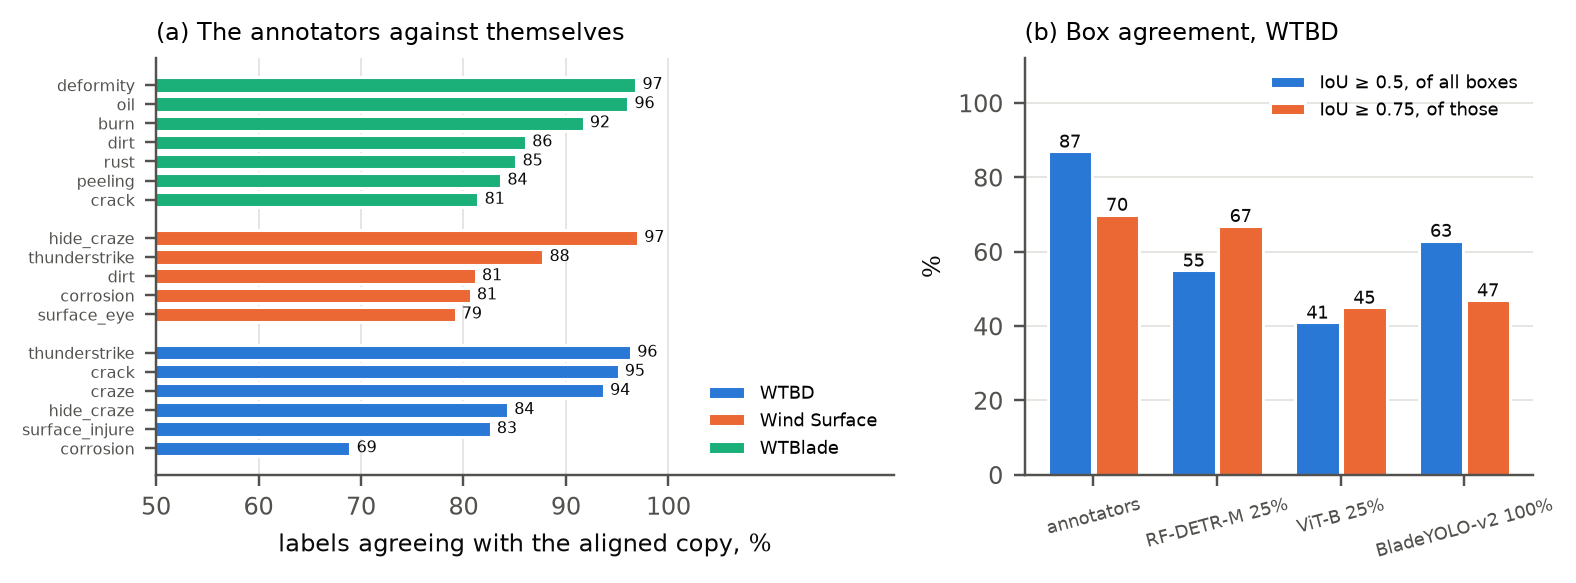
\includegraphics[width=0.94\linewidth,height=\textheight,keepaspectratio,alt={Figure 17. (a) Per-class agreement on aligned copies. (b) Box agreement on WTBD: how often an independent annotator's box, or a detector's best box, reaches IoU 0.5, and of those, how many reach 0.75. Conf ≥ 0.1 for detectors. RF-DETR-M at 25\% labels matches the annotators on extent once it finds a defect (0.67 against 0.70; median IoU 0.83 for both).}]{figures/fig12_label_agreement.png}
\caption{Figure 17. (a) Per-class agreement on aligned copies. (b) Box
agreement on WTBD: how often an independent annotator's box, or a
detector's best box, reaches IoU 0.5, and of those, how many reach 0.75.
Conf ≥ 0.1 for detectors. RF-DETR-M at 25\% labels matches the
annotators on extent once it finds a defect (0.67 against 0.70; median
IoU 0.83 for both).}
\end{figure}

\subsection{Box granularity}\label{box-granularity}

On WTBD-group, tolerant AP50 exceeds standard AP50 by +11.9 for
BladeYOLO-v2 (56.1 → 68.0) and +12.4 for YOLO12-L (40.0 → 52.4). Most
striking is craze, from 9.9 to 66.1. All 15 craze test images are
rotated, flipped or recoloured copies of one long leading-edge split,
annotated as 2--3 segment boxes (Fig.~18). The same effect holds for
RF-DETR scored with classes merged: AP50 rises from 66.1 to 79.7 on
WTBD-group and from 50.1 to 61.2 on WTBlade-group (Table~15).

\begin{figure}
\centering
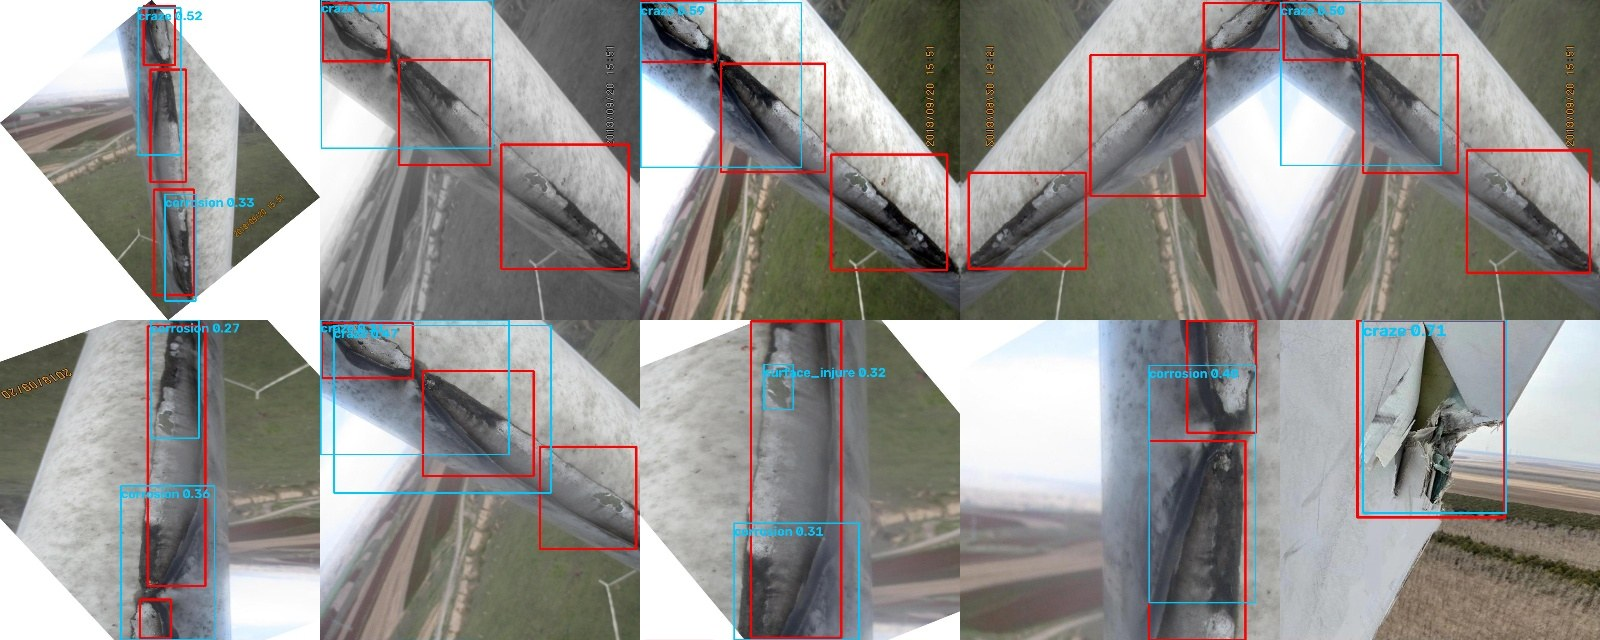
\includegraphics[width=0.78\linewidth,height=\textheight,keepaspectratio,alt={Figure 18. All 15 WTBD-group craze test images come from one scene. Red: labels, split into segments by the annotator. Blue: BladeYOLO-v2 predictions. The model often draws one box where the label has several, which counts as an error at IoU 0.5 and explains most of the ``craze failure''.}]{figures/fig13_craze_scene.jpg}
\caption{Figure 18. All 15 WTBD-group craze test images come from one
scene. Red: labels, split into segments by the annotator. Blue:
BladeYOLO-v2 predictions. The model often draws one box where the label
has several, which counts as an error at IoU 0.5 and explains most of
the ``craze failure''.}
\end{figure}

Table~11 gives the per-class view for BladeYOLO-v2.

\begin{longtable}[]{@{}
  >{\raggedright\arraybackslash}p{(\linewidth - 6\tabcolsep) * \real{0.2500}}
  >{\raggedright\arraybackslash}p{(\linewidth - 6\tabcolsep) * \real{0.2500}}
  >{\raggedright\arraybackslash}p{(\linewidth - 6\tabcolsep) * \real{0.2500}}
  >{\raggedright\arraybackslash}p{(\linewidth - 6\tabcolsep) * \real{0.2500}}@{}}
\caption{Table 11. Three box scores on WTBD-group test, in percent (500
scene replicates). Per class: BladeYOLO-v2. The official-split rows use
the same scores, and the official-minus-group gap shrinks as the metric
becomes split-invariant (BladeYOLO-v2: +25.4, +20.9,
+16.8).}\tabularnewline
\toprule\noalign{}
\begin{minipage}[b]{\linewidth}\raggedright
\end{minipage} & \begin{minipage}[b]{\linewidth}\raggedright
standard AP50
\end{minipage} & \begin{minipage}[b]{\linewidth}\raggedright
tolerant AP50
\end{minipage} & \begin{minipage}[b]{\linewidth}\raggedright
region AP
\end{minipage} \\
\midrule\noalign{}
\endfirsthead
\toprule\noalign{}
\begin{minipage}[b]{\linewidth}\raggedright
\end{minipage} & \begin{minipage}[b]{\linewidth}\raggedright
standard AP50
\end{minipage} & \begin{minipage}[b]{\linewidth}\raggedright
tolerant AP50
\end{minipage} & \begin{minipage}[b]{\linewidth}\raggedright
region AP
\end{minipage} \\
\midrule\noalign{}
\endhead
\bottomrule\noalign{}
\endlastfoot
BladeYOLO-v2, WTBD-group & 56.1 {[}48.3, 79.1{]} & 68.0 {[}60.4, 83.1{]}
& 60.3 {[}55.2, 74.3{]} \\
YOLO12-L, WTBD-group & 40.0 {[}33.9, 67.8{]} & 52.4 {[}46.5, 74.0{]} &
44.1 {[}40.2, 59.2{]} \\
difference & +16.1 {[}+2.3, +28.4{]} & +15.6 {[}+0.1, +23.7{]} &
\textbf{+16.2 {[}+7.7, +23.6{]}} \\
BladeYOLO-v2, WTBD official & 81.5 & 88.9 & 77.1 \\
YOLO12-L, WTBD official & 69.0 & 80.0 & 66.6 \\
craze & 9.9 & \textbf{66.1} & 42.7 \\
corrosion & 62.6 & 67.6 & 68.4 \\
surface\_injure & 75.9 & 81.6 & 68.9 \\
thunderstrike & 100.0 & 100.0 & 68.2 \\
crack & 35.2 & 35.6 & 49.1 \\
hide\_craze & 53.0 & 56.8 & 64.5 \\
\end{longtable}

Two limits apply. We hypothesised that part of the leakage inflation is
memorised box splitting, and tested it: the tolerant gain is not smaller
on test images with a training twin, so the hypothesis is not supported.
And training a detector to tolerate splitting does not help overall:
blanket split-tolerant training is not an improvement (tolerant AP50
+1.5 {[}−11.1, +6.4{]}), and class-selective tolerance raises corrosion
by +9.3 {[}−0.3, +24.6{]} while the mean moves by −0.4. So the ambiguity
limits what can be measured more than what can be trained away.

\textbf{Annotators as a ceiling.} Corrosion copies agree on only 69\% of
labels and models score near that (BladeYOLO-v2 AP50 54--63), so more
corrosion ``improvement'' is largely unmeasurable with these labels.
Crack copies agree on 95\% while the YOLO family scores 35--39, so crack
is a genuine model weakness there.

\subsection{Subset luck}\label{subset-luck}

At a fixed budget of 25\% of scenes, which scenes are labelled matters
more than any model effect we measured (Fig.~19). Across 8 random draws,
with the same model, recipe and seed, ViT-B test mAP50-95 spans
9.0--19.6 (×2.2), and without DINOv3 it spans 2.6--7.2. The DINOv3 gain
holds on 8 of 8 draws (+7.1 {[}+5.1, +12.6{]}), and draw quality carries
over between models (Spearman ρ 0.71). Yet no label-free subset property
we tested predicts it (H7, G16, H20). Label-free scene selection by
patch coverage beats random by +5.2 {[}+1.9, +10.5{]} but does not
separate from FreeSel {[}\citeproc{ref-freesel}{30}{]} (+2.1 {[}−1.2,
+9.1{]}, P 0.917, validation opposite).

Table~12 gives the selection runs at the same 25\% budget. Selecting by
class balance does worst of the five arms, which suggests that which
scenes are labelled matters more than matching class counts.

\begin{longtable}[]{@{}
  >{\raggedright\arraybackslash}p{(\linewidth - 8\tabcolsep) * \real{0.2000}}
  >{\raggedright\arraybackslash}p{(\linewidth - 8\tabcolsep) * \real{0.2000}}
  >{\raggedright\arraybackslash}p{(\linewidth - 8\tabcolsep) * \real{0.2000}}
  >{\raggedright\arraybackslash}p{(\linewidth - 8\tabcolsep) * \real{0.2000}}
  >{\raggedright\arraybackslash}p{(\linewidth - 8\tabcolsep) * \real{0.2000}}@{}}
\caption{Table 12. Selection of which 25\% of WTBD-group scenes to
label: 18 ViT-B runs at the same budget, training seed 0 unless noted.
Random draws per run: 11.2, 13.5, 11.8, 12.3, 9.0, 10.0, 12.4,
19.6.}\tabularnewline
\toprule\noalign{}
\begin{minipage}[b]{\linewidth}\raggedright
arm (runs)
\end{minipage} & \begin{minipage}[b]{\linewidth}\raggedright
test mAP50
\end{minipage} & \begin{minipage}[b]{\linewidth}\raggedright
test mAP50-95
\end{minipage} & \begin{minipage}[b]{\linewidth}\raggedright
val mAP50-95
\end{minipage} & \begin{minipage}[b]{\linewidth}\raggedright
rank among 8 random (test / val)
\end{minipage} \\
\midrule\noalign{}
\endfirsthead
\toprule\noalign{}
\begin{minipage}[b]{\linewidth}\raggedright
arm (runs)
\end{minipage} & \begin{minipage}[b]{\linewidth}\raggedright
test mAP50
\end{minipage} & \begin{minipage}[b]{\linewidth}\raggedright
test mAP50-95
\end{minipage} & \begin{minipage}[b]{\linewidth}\raggedright
val mAP50-95
\end{minipage} & \begin{minipage}[b]{\linewidth}\raggedright
rank among 8 random (test / val)
\end{minipage} \\
\midrule\noalign{}
\endhead
\bottomrule\noalign{}
\endlastfoot
patch coverage, label-free (4) & 40.6 & \textbf{17.7} & 23.6 & 2 of 9 /
3 of 9 \\
FreeSel-224 (2) & 42.9 & 15.6 & \textbf{27.1} & 2 of 9 / 1 of 9 \\
FreeSel-640 (2) & 34.4 & 14.5 & 26.6 & 2 of 9 / 2 of 9 \\
random (8) & 31.3 & 12.5 & 21.6 & \\
class-matched, uses labels (2) & 25.3 & 10.4 & 19.7 & 7 of 9 / 7 of 9 \\
\end{longtable}

\begin{figure}
\centering
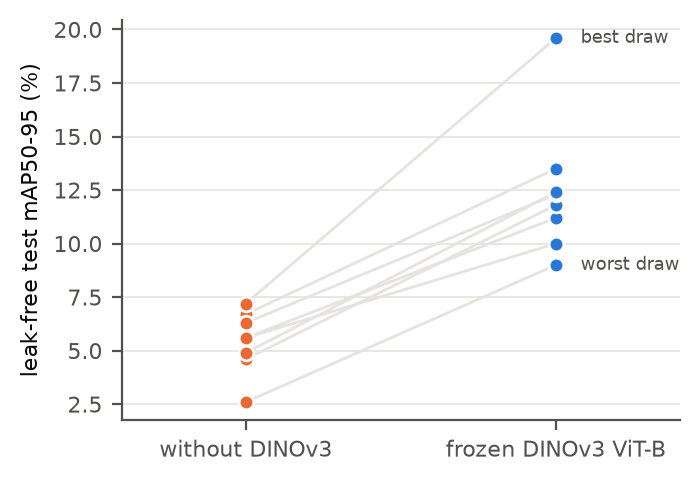
\includegraphics[width=0.72\linewidth,height=\textheight,keepaspectratio,alt={Figure 19. Subset luck: test mAP50-95 across random 25\% scene draws, same model, recipe and seed.}]{figures/fig5_subset_luck.png}
\caption{Figure 19. Subset luck: test mAP50-95 across random 25\% scene
draws, same model, recipe and seed.}
\end{figure}

\subsection{Error anatomy}\label{error-anatomy}

Scarce labels fail differently by detector family (Fig.~20, in the style
of TIDE {[}\citeproc{ref-tide}{40}{]}). For each test box we ask whether
a same-class box at IoU ≥ 0.5 is among the outputs and how it is scored.

\begin{figure}
\centering
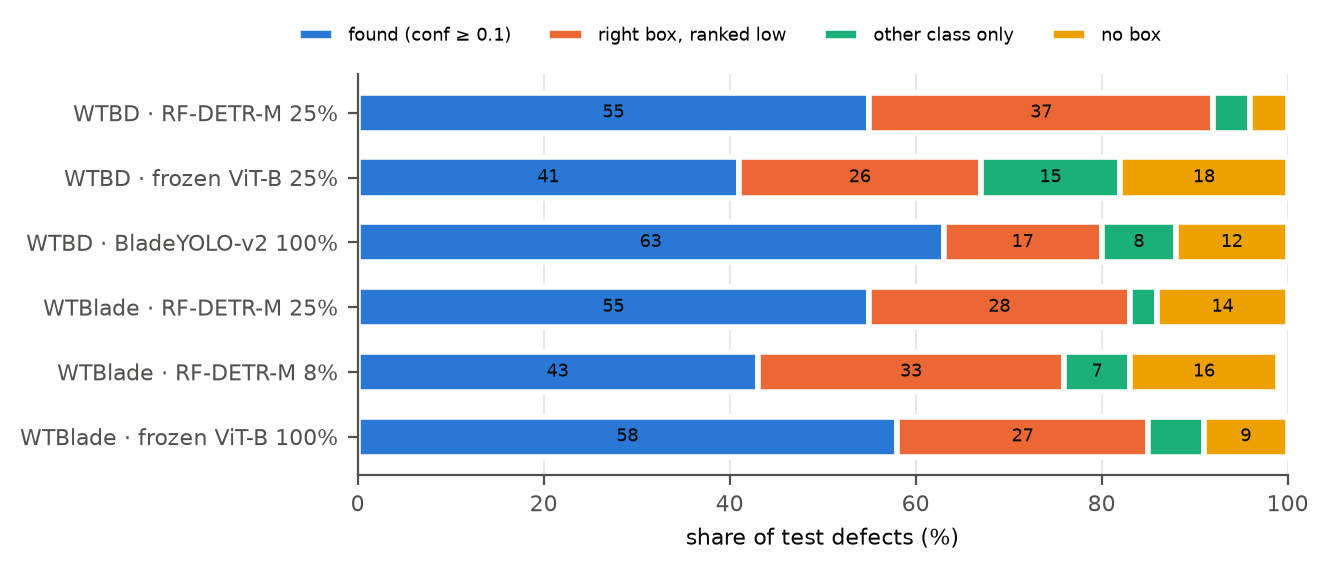
\includegraphics[width=0.84\linewidth,height=\textheight,keepaspectratio,alt={Figure 20. Error anatomy. Hit: same-class box at IoU ≥ 0.5 with confidence ≥ 0.1. Ranked low: such a box exists only below 0.1. Other class: only other-class boxes at IoU ≥ 0.5. No box: nothing at IoU ≥ 0.5.}]{figures/fig6_error_anatomy.png}
\caption{Figure 20. Error anatomy. Hit: same-class box at IoU ≥ 0.5 with
confidence ≥ 0.1. Ranked low: such a box exists only below 0.1. Other
class: only other-class boxes at IoU ≥ 0.5. No box: nothing at IoU ≥
0.5.}
\end{figure}

Table~13 gives the numbers and Table~14 the extent comparison.

\begin{longtable}[]{@{}
  >{\raggedright\arraybackslash}p{(\linewidth - 14\tabcolsep) * \real{0.1250}}
  >{\raggedright\arraybackslash}p{(\linewidth - 14\tabcolsep) * \real{0.1250}}
  >{\raggedright\arraybackslash}p{(\linewidth - 14\tabcolsep) * \real{0.1250}}
  >{\raggedright\arraybackslash}p{(\linewidth - 14\tabcolsep) * \real{0.1250}}
  >{\raggedright\arraybackslash}p{(\linewidth - 14\tabcolsep) * \real{0.1250}}
  >{\raggedright\arraybackslash}p{(\linewidth - 14\tabcolsep) * \real{0.1250}}
  >{\raggedright\arraybackslash}p{(\linewidth - 14\tabcolsep) * \real{0.1250}}
  >{\raggedright\arraybackslash}p{(\linewidth - 14\tabcolsep) * \real{0.1250}}@{}}
\caption{Table 13. Error anatomy, as a share of test boxes. Candidate
recall = hit + ranked low. YOLO-family runs keep fewer boxes after NMS
(about 50--80 per image) than RF-DETR (about 300), so recall within each
image's top 50 boxes is also given.}\tabularnewline
\toprule\noalign{}
\begin{minipage}[b]{\linewidth}\raggedright
dataset
\end{minipage} & \begin{minipage}[b]{\linewidth}\raggedright
detector
\end{minipage} & \begin{minipage}[b]{\linewidth}\raggedright
hit
\end{minipage} & \begin{minipage}[b]{\linewidth}\raggedright
ranked low
\end{minipage} & \begin{minipage}[b]{\linewidth}\raggedright
other class
\end{minipage} & \begin{minipage}[b]{\linewidth}\raggedright
no box
\end{minipage} & \begin{minipage}[b]{\linewidth}\raggedright
candidate recall
\end{minipage} & \begin{minipage}[b]{\linewidth}\raggedright
in top 50
\end{minipage} \\
\midrule\noalign{}
\endfirsthead
\toprule\noalign{}
\begin{minipage}[b]{\linewidth}\raggedright
dataset
\end{minipage} & \begin{minipage}[b]{\linewidth}\raggedright
detector
\end{minipage} & \begin{minipage}[b]{\linewidth}\raggedright
hit
\end{minipage} & \begin{minipage}[b]{\linewidth}\raggedright
ranked low
\end{minipage} & \begin{minipage}[b]{\linewidth}\raggedright
other class
\end{minipage} & \begin{minipage}[b]{\linewidth}\raggedright
no box
\end{minipage} & \begin{minipage}[b]{\linewidth}\raggedright
candidate recall
\end{minipage} & \begin{minipage}[b]{\linewidth}\raggedright
in top 50
\end{minipage} \\
\midrule\noalign{}
\endhead
\bottomrule\noalign{}
\endlastfoot
WTBD & RF-DETR-M 25\% (4 subsets) & 0.55 & \textbf{0.37} & 0.04 & 0.04 &
\textbf{0.92} & 0.81 \\
WTBD & ViT-B 25\% (4 subsets) & 0.41 & 0.26 & 0.15 & 0.18 & 0.67 &
0.66 \\
WTBD & BladeYOLO-v2 100\% (2 seeds) & 0.63 & 0.17 & 0.08 & 0.12 & 0.80 &
0.80 \\
WTBlade & RF-DETR-M 25\% (4 subsets) & 0.55 & 0.28 & 0.03 & 0.14 &
\textbf{0.83} & 0.72 \\
WTBlade & RF-DETR-M 8\% (4 subsets) & 0.43 & 0.33 & 0.07 & 0.16 & 0.77 &
0.62 \\
WTBlade & ViT-B 100\% & 0.58 & 0.27 & 0.06 & 0.09 & 0.85 & 0.81 \\
\end{longtable}

\begin{longtable}[]{@{}
  >{\raggedright\arraybackslash}p{(\linewidth - 10\tabcolsep) * \real{0.1667}}
  >{\raggedright\arraybackslash}p{(\linewidth - 10\tabcolsep) * \real{0.1667}}
  >{\raggedright\arraybackslash}p{(\linewidth - 10\tabcolsep) * \real{0.1667}}
  >{\raggedright\arraybackslash}p{(\linewidth - 10\tabcolsep) * \real{0.1667}}
  >{\raggedright\arraybackslash}p{(\linewidth - 10\tabcolsep) * \real{0.1667}}
  >{\raggedright\arraybackslash}p{(\linewidth - 10\tabcolsep) * \real{0.1667}}@{}}
\caption{Table 14. Box extent against the annotator ceiling on WTBD
(same-class IoU of a label with its copy, or of the best prediction with
conf ≥ 0.1, per test box). RF-DETR-M's gap is in finding defects; once
found, its boxes match labels as well as a second annotator's do. The
YOLO-family runs were extent-limited.}\tabularnewline
\toprule\noalign{}
\begin{minipage}[b]{\linewidth}\raggedright
source
\end{minipage} & \begin{minipage}[b]{\linewidth}\raggedright
boxes
\end{minipage} & \begin{minipage}[b]{\linewidth}\raggedright
IoU ≥ 0.5
\end{minipage} & \begin{minipage}[b]{\linewidth}\raggedright
of those, IoU ≥ 0.75
\end{minipage} & \begin{minipage}[b]{\linewidth}\raggedright
median IoU of those
\end{minipage} & \begin{minipage}[b]{\linewidth}\raggedright
IoU ≥ 0.75
\end{minipage} \\
\midrule\noalign{}
\endfirsthead
\toprule\noalign{}
\begin{minipage}[b]{\linewidth}\raggedright
source
\end{minipage} & \begin{minipage}[b]{\linewidth}\raggedright
boxes
\end{minipage} & \begin{minipage}[b]{\linewidth}\raggedright
IoU ≥ 0.5
\end{minipage} & \begin{minipage}[b]{\linewidth}\raggedright
of those, IoU ≥ 0.75
\end{minipage} & \begin{minipage}[b]{\linewidth}\raggedright
median IoU of those
\end{minipage} & \begin{minipage}[b]{\linewidth}\raggedright
IoU ≥ 0.75
\end{minipage} \\
\midrule\noalign{}
\endhead
\bottomrule\noalign{}
\endlastfoot
annotators, all copies & 2,965 & 0.87 & 0.70 & 0.83 & 0.61 \\
annotators, test copies & 392 & 0.91 & 0.75 & 0.84 & 0.68 \\
RF-DETR-M 25\% (4 subsets) & 940 & 0.55 & 0.67 & 0.83 & 0.37 \\
ViT-B 25\% (4 subsets) & 940 & 0.41 & 0.45 & 0.73 & 0.19 \\
BladeYOLO-v2 100\% & 235 & 0.63 & 0.47 & 0.74 & 0.29 \\
\end{longtable}

\begin{itemize}
\tightlist
\item
  \textbf{RF-DETR at 25\% labels proposes the right box for most
  defects.} Candidate recall is 0.92 on WTBD (above BladeYOLO-v2 at
  100\%, 0.80) and 0.83 on WTBlade. Its deficit is scoring: 37\% of WTBD
  test defects have a correct box scored below 0.1.
\item
  \textbf{On WTBD the rare classes are confused}, with crack missed or
  mislabelled and thunderstrike found under other classes (54\% located
  as another class, in 4 subsets). On WTBlade, 43--49\% of crack boxes
  lack a same-class box at IoU ≥ 0.5 at every budget (RF-DETR 8\%: 0.47;
  25\%: 0.49; ViT-B 100\%: 0.43). So this is not a label-budget problem.
  Misses concentrate on small boxes (1.00 below 16 px, 0.65 below 32 px,
  0.22 above 64 px), and among near-misses the largest share is shifted
  boxes (44\%), not split ones.
\item
  \textbf{Not resolution, on WTBD.} Median defect short sides at 640 px
  are 62--148 px by class.
\end{itemize}

\section{Leave-one-dataset-out: data volume does not replace target
labels}\label{sec:lodo}

If label count were the bottleneck, pooling every other blade dataset
should help. G28 tests this directly. It was pre-registered before any
pool was built or run started.

\subsection{Design}\label{design}

For each target T, two class-agnostic RF-DETR-M arms (640 px, cosine,
seed 0) are scored on T's test set:

\begin{itemize}
\tightlist
\item
  \textbf{ID-T:} T's group train (WTBD 100 epochs, WTBlade 60).
\item
  \textbf{X-T:} every other source, twin-free against \emph{all} of T,
  12 epochs. Selection uses a held-out 5\% of X-T's own images
  {[}\citeproc{ref-domainbed}{32}{]}; T is never seen, not even for
  selection.
\end{itemize}

Every image of T is an evaluation key for the twin rule: same file,
DINOv2 ≥ 0.90, ORB ≥ 25 inliers, pixel correlation ≥ 0.97 over 8
orientations, and the closure of all of these. GAN images and box-less
images are dropped. The rule deliberately sits below the audit's twin
thresholds (0.93 and 0.99): earlier versions of this rule, on the G27
pool, kept 830 pixel twins and then neighbouring video frames, and each
failure was logged and fixed before any training. Fig.~21 shows the
result: X-WTBD has 26,065 training images (55,845 boxes across its train
and held-out images) and X-WTBlade 14,405 (27,844). Fig.~22 shows the
closest pairs an independent audit could find; the highest pixel
correlation and cosine to any target image are 0.964 / 0.827 and 0.970 /
0.900.

\begin{figure}
\centering
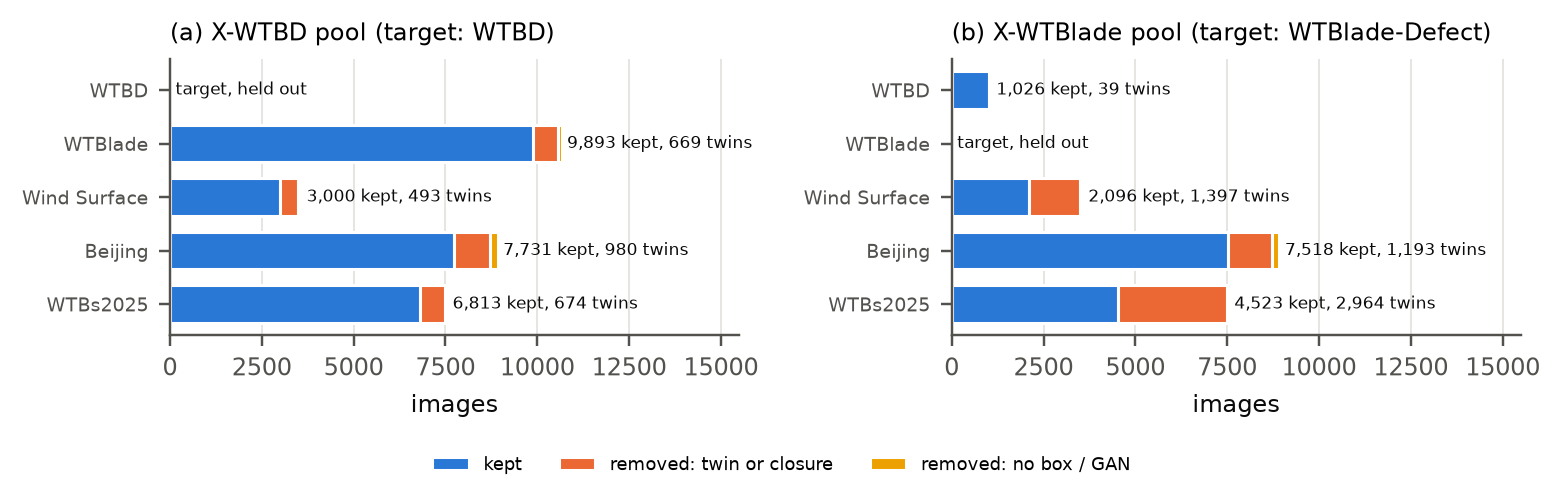
\includegraphics[width=0.9\linewidth,height=\textheight,keepaspectratio,alt={Figure 21. Composition of the G28 pools: images kept from each source and removed by the twin rule. For X-WTBlade, 2,964 WTBs2025 images are removed, since that dataset contains WTBlade-Defect's images.}]{figures/fig20_pools.png}
\caption{Figure 21. Composition of the G28 pools: images kept from each
source and removed by the twin rule. For X-WTBlade, 2,964 WTBs2025
images are removed, since that dataset contains WTBlade-Defect's
images.}
\end{figure}

\begin{figure}
\centering
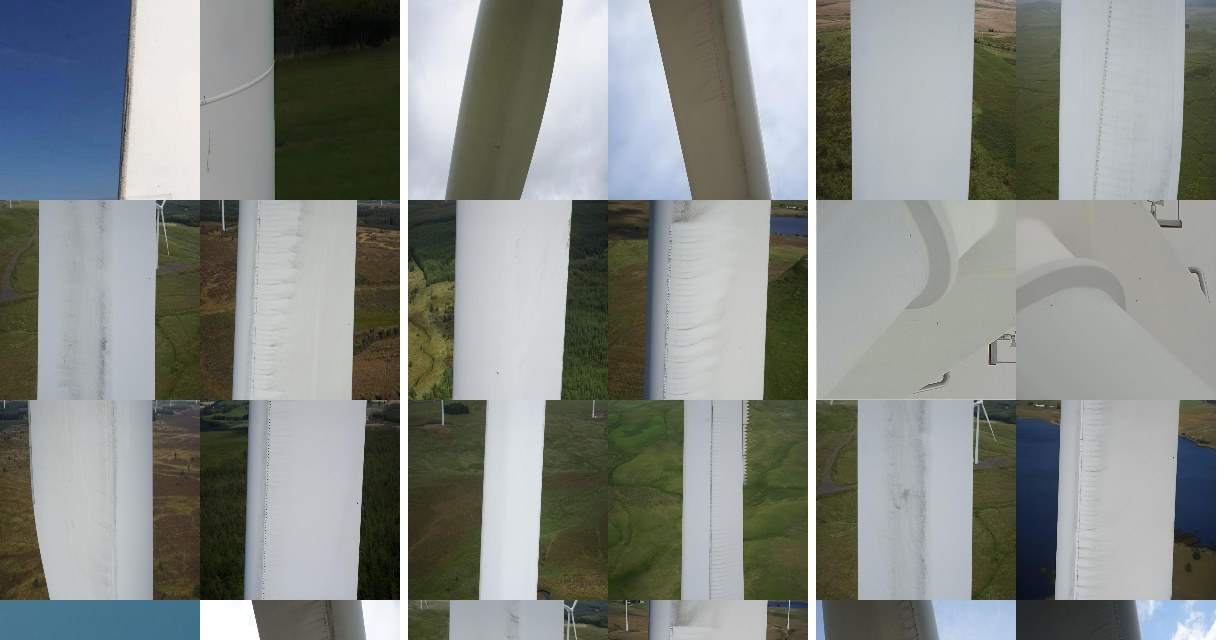
\includegraphics[width=0.72\linewidth,height=\textheight,keepaspectratio,alt={Figure 22. Independent audit of the X-WTBlade pool: the closest remaining pairs by pixel correlation between a kept pool image and a target image. By eye these are similar blades, not copies. The same physical defect from another flight cannot be excluded without capture metadata.}]{figures/fig21_pool_audit.jpg}
\caption{Figure 22. Independent audit of the X-WTBlade pool: the closest
remaining pairs by pixel correlation between a kept pool image and a
target image. By eye these are similar blades, not copies. The same
physical defect from another flight cannot be excluded without capture
metadata.}
\end{figure}

We define the gaps \(G_{\mathrm{std}} = \mathrm{ID} - \mathrm{X}\) in
standard AP50 and \(G_{\mathrm{reg}} = \mathrm{ID} - \mathrm{X}\) in
region AP, and the convention share
\(1 - G_{\mathrm{reg}} / G_{\mathrm{std}}\), the part of the gap that is
about how boxes are drawn. The direction counted as alive only if, on
\emph{both} targets, X reached at least 0.80 × ID in region AP and the
convention share was at least 0.5. Both bars were judgment calls fixed
before any number existed.

\subsection{Results}\label{results}

\begin{longtable}[]{@{}
  >{\raggedright\arraybackslash}p{(\linewidth - 14\tabcolsep) * \real{0.1250}}
  >{\raggedright\arraybackslash}p{(\linewidth - 14\tabcolsep) * \real{0.1250}}
  >{\raggedright\arraybackslash}p{(\linewidth - 14\tabcolsep) * \real{0.1250}}
  >{\raggedright\arraybackslash}p{(\linewidth - 14\tabcolsep) * \real{0.1250}}
  >{\raggedright\arraybackslash}p{(\linewidth - 14\tabcolsep) * \real{0.1250}}
  >{\raggedright\arraybackslash}p{(\linewidth - 14\tabcolsep) * \real{0.1250}}
  >{\raggedright\arraybackslash}p{(\linewidth - 14\tabcolsep) * \real{0.1250}}
  >{\raggedright\arraybackslash}p{(\linewidth - 14\tabcolsep) * \real{0.1250}}@{}}
\caption{Table 15. G28, class-agnostic, test, scene bootstrap (2,000
replicates). \emph{Ref} is G27 A0 (class-aware, 768 / 640 px), scored
with classes merged; reported, not decisive. \emph{Trivial} is one box
over the whole image.}\tabularnewline
\toprule\noalign{}
\begin{minipage}[b]{\linewidth}\raggedright
target
\end{minipage} & \begin{minipage}[b]{\linewidth}\raggedright
arm
\end{minipage} & \begin{minipage}[b]{\linewidth}\raggedright
train images
\end{minipage} & \begin{minipage}[b]{\linewidth}\raggedright
AP50
\end{minipage} & \begin{minipage}[b]{\linewidth}\raggedright
AP50-95
\end{minipage} & \begin{minipage}[b]{\linewidth}\raggedright
tolerant AP50
\end{minipage} & \begin{minipage}[b]{\linewidth}\raggedright
region AP
\end{minipage} & \begin{minipage}[b]{\linewidth}\raggedright
AR50
\end{minipage} \\
\midrule\noalign{}
\endfirsthead
\toprule\noalign{}
\begin{minipage}[b]{\linewidth}\raggedright
target
\end{minipage} & \begin{minipage}[b]{\linewidth}\raggedright
arm
\end{minipage} & \begin{minipage}[b]{\linewidth}\raggedright
train images
\end{minipage} & \begin{minipage}[b]{\linewidth}\raggedright
AP50
\end{minipage} & \begin{minipage}[b]{\linewidth}\raggedright
AP50-95
\end{minipage} & \begin{minipage}[b]{\linewidth}\raggedright
tolerant AP50
\end{minipage} & \begin{minipage}[b]{\linewidth}\raggedright
region AP
\end{minipage} & \begin{minipage}[b]{\linewidth}\raggedright
AR50
\end{minipage} \\
\midrule\noalign{}
\endhead
\bottomrule\noalign{}
\endlastfoot
WTBD-group & ID & 745 & 72.9 {[}57.6, 86.3{]} & 41.9 & 84.6 & 68.9
{[}61.3, 75.4{]} & 98.7 \\
& X & 26,065 & \textbf{17.7} {[}11.9, 28.4{]} & 6.0 & 24.2 & 43.6
{[}37.4, 52.3{]} & 79.6 \\
& ref & 745 & 66.1 & 40.5 & 79.7 & 65.9 & 97.9 \\
& trivial & & 0.0 & & & 14.0 & \\
WTBlade-group & ID & 2,136 & 51.7 {[}48.0, 58.8{]} & 21.5 & 65.1 & 68.7
{[}62.6, 75.2{]} & 90.5 \\
& X & 14,405 & \textbf{2.4} {[}0.8, 3.5{]} & 0.5 & 3.2 & 37.6 {[}32.5,
45.1{]} & 38.2 \\
& ref & 2,136 & 50.1 & 21.3 & 61.2 & 68.0 & 92.2 \\
& trivial & & 1.0 & & & 24.2 & \\
\end{longtable}

\begin{longtable}[]{@{}
  >{\raggedright\arraybackslash}p{(\linewidth - 10\tabcolsep) * \real{0.1667}}
  >{\raggedright\arraybackslash}p{(\linewidth - 10\tabcolsep) * \real{0.1667}}
  >{\raggedright\arraybackslash}p{(\linewidth - 10\tabcolsep) * \real{0.1667}}
  >{\raggedright\arraybackslash}p{(\linewidth - 10\tabcolsep) * \real{0.1667}}
  >{\raggedright\arraybackslash}p{(\linewidth - 10\tabcolsep) * \real{0.1667}}
  >{\raggedright\arraybackslash}p{(\linewidth - 10\tabcolsep) * \real{0.1667}}@{}}
\caption{Table 16. G28 decision. Bars: ratio ≥ 0.80 and share ≥ 0.5 on
both targets. ID − X has P(\textgreater{} 0) = 1.000 on every metric of
both targets.}\tabularnewline
\toprule\noalign{}
\begin{minipage}[b]{\linewidth}\raggedright
target
\end{minipage} & \begin{minipage}[b]{\linewidth}\raggedright
X / ID region AP
\end{minipage} & \begin{minipage}[b]{\linewidth}\raggedright
convention share
\end{minipage} & \begin{minipage}[b]{\linewidth}\raggedright
\(G_{\mathrm{std}}\) {[}95\% CI{]}
\end{minipage} & \begin{minipage}[b]{\linewidth}\raggedright
\(G_{\mathrm{reg}}\) {[}95\% CI{]}
\end{minipage} & \begin{minipage}[b]{\linewidth}\raggedright
verdict
\end{minipage} \\
\midrule\noalign{}
\endfirsthead
\toprule\noalign{}
\begin{minipage}[b]{\linewidth}\raggedright
target
\end{minipage} & \begin{minipage}[b]{\linewidth}\raggedright
X / ID region AP
\end{minipage} & \begin{minipage}[b]{\linewidth}\raggedright
convention share
\end{minipage} & \begin{minipage}[b]{\linewidth}\raggedright
\(G_{\mathrm{std}}\) {[}95\% CI{]}
\end{minipage} & \begin{minipage}[b]{\linewidth}\raggedright
\(G_{\mathrm{reg}}\) {[}95\% CI{]}
\end{minipage} & \begin{minipage}[b]{\linewidth}\raggedright
verdict
\end{minipage} \\
\midrule\noalign{}
\endhead
\bottomrule\noalign{}
\endlastfoot
WTBD-group & 0.63 & 0.54 & +55.2 {[}+41.7, +66.4{]} & +25.3 {[}+14.4,
+33.9{]} & dead \\
WTBlade-group & 0.55 & 0.37 & +49.3 {[}+45.0, +57.2{]} & +31.0 {[}+26.8,
+34.6{]} & dead \\
\end{longtable}

\begin{figure}
\centering
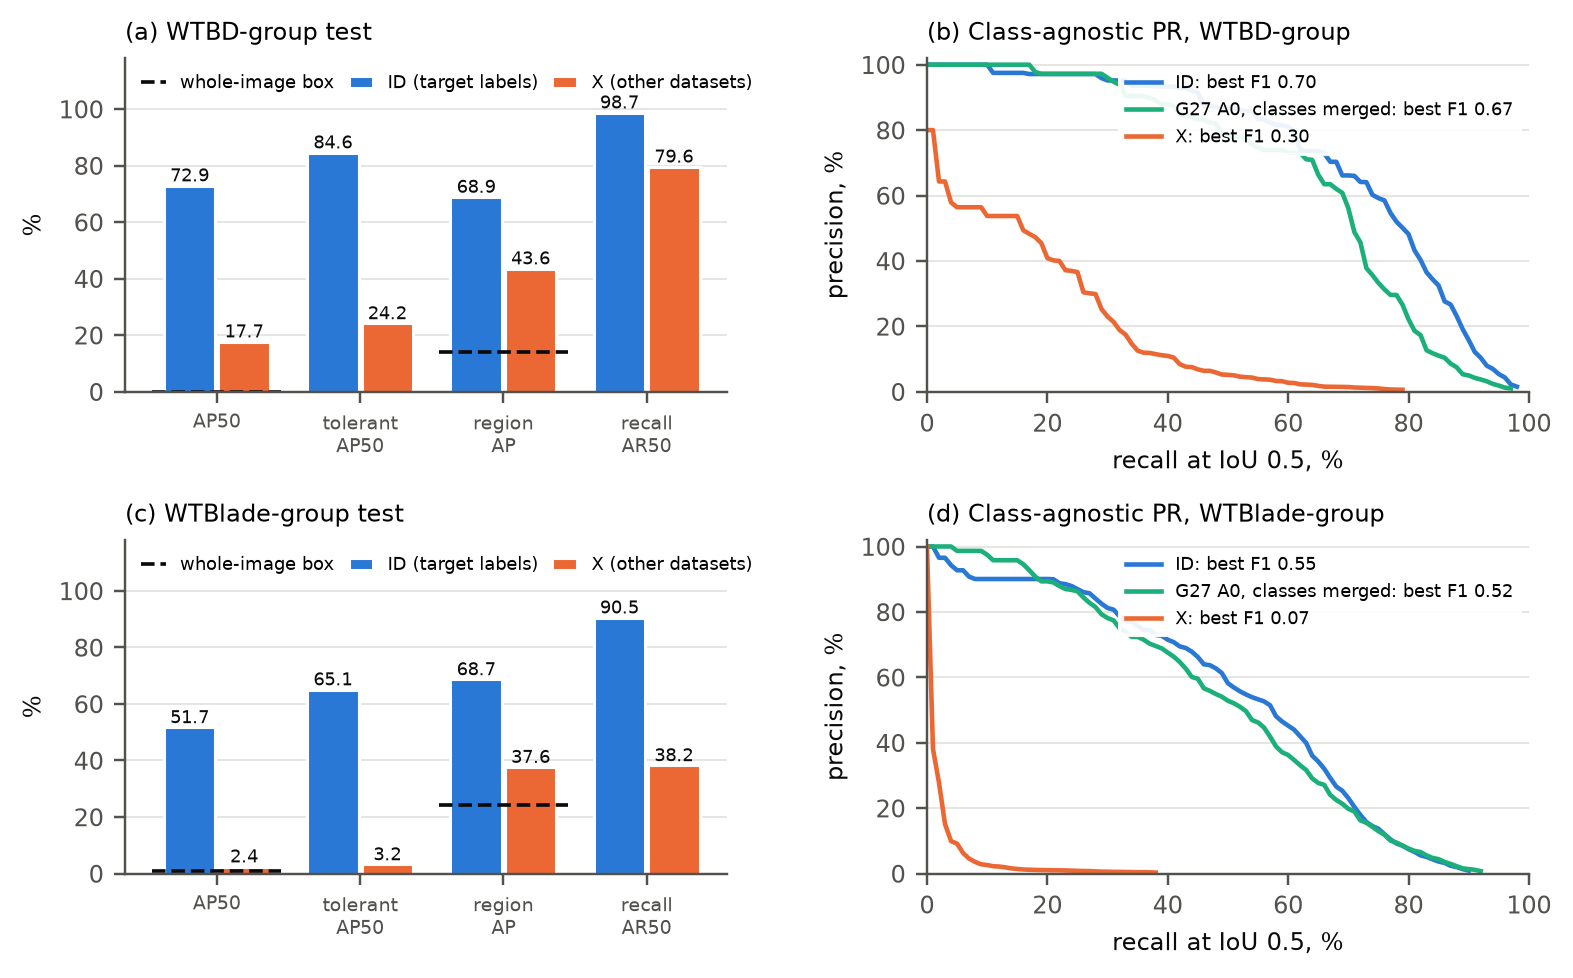
\includegraphics[width=0.98\linewidth,height=\textheight,keepaspectratio,alt={Figure 23. G28. (a, c) ID and X on target test; dashed lines mark a trivial whole-image detector. (b, d) Class-agnostic precision--recall at IoU 0.5.}]{figures/fig18_g28.png}
\caption{Figure 23. G28. (a, c) ID and X on target test; dashed lines
mark a trivial whole-image detector. (b, d) Class-agnostic
precision--recall at IoU 0.5.}
\end{figure}

\begin{figure}
\centering
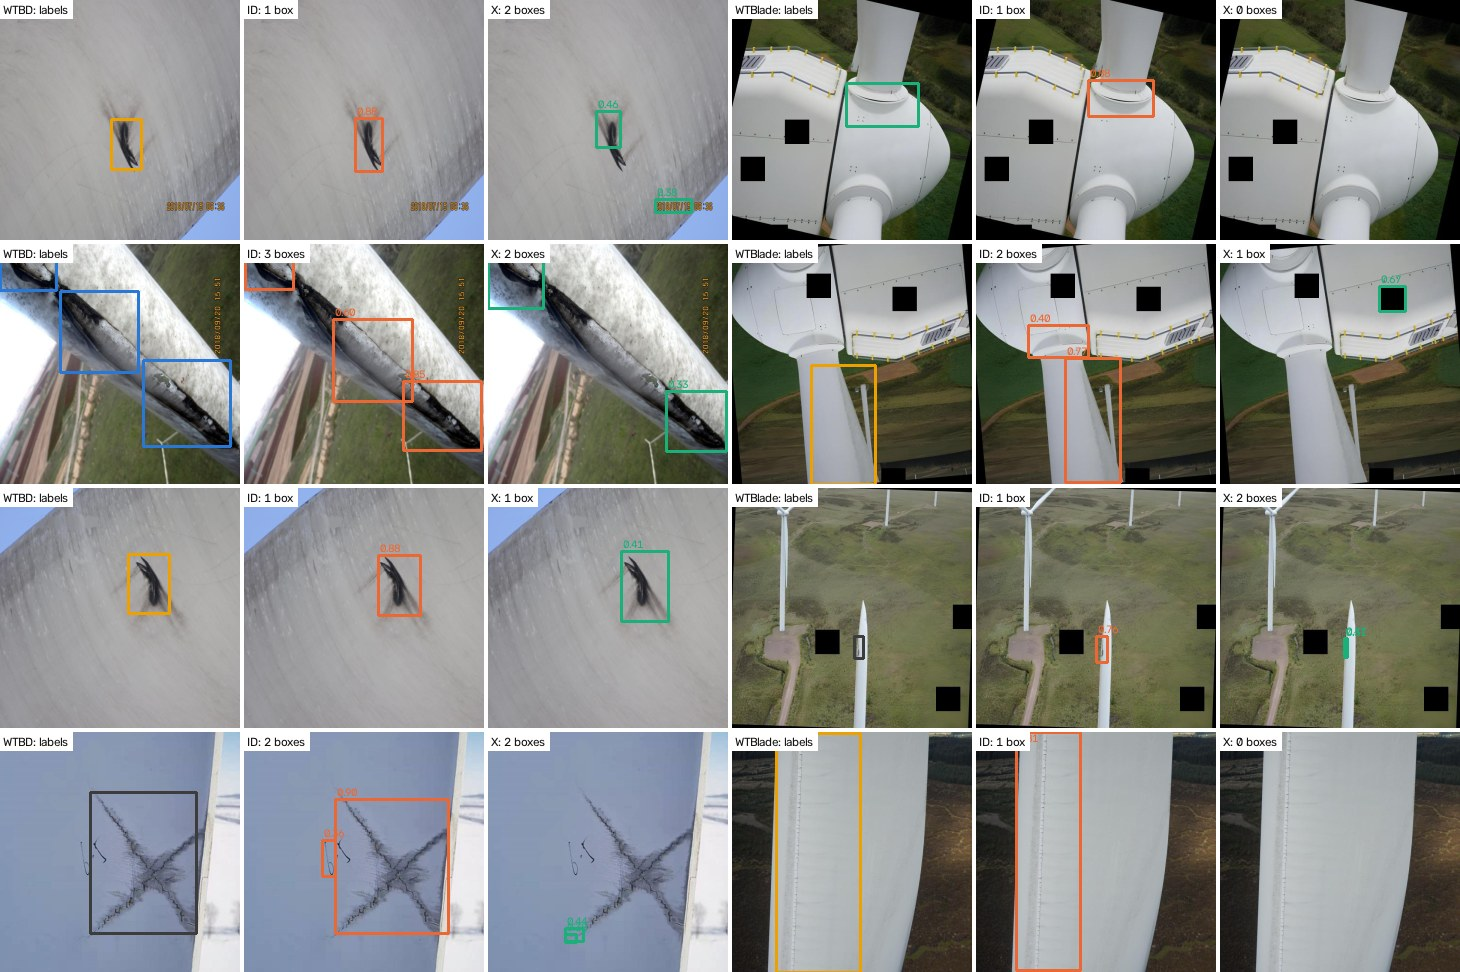
\includegraphics[width=1\linewidth,height=\textheight,keepaspectratio,alt={Figure 24. Labels, ID and X on random test images (fixed seed), boxes with confidence ≥ 0.3. Left three columns: WTBD-group. Right three: WTBlade-group. X often has the right area or a nearby distractor; it also returns nothing on images where ID is correct. Black squares in WTBlade-group are offline cutout from the Roboflow export, which the frames retain.}]{figures/fig19_predictions.jpg}
\caption{Figure 24. Labels, ID and X on random test images (fixed seed),
boxes with confidence ≥ 0.3. Left three columns: WTBD-group. Right
three: WTBlade-group. X often has the right area or a nearby distractor;
it also returns nothing on images where ID is correct. Black squares in
WTBlade-group are offline cutout from the Roboflow export, which the
frames retain.}
\end{figure}

\textbf{The direction fails on both targets.} Table~15, Table~16 and
Fig.~23 give the numbers, and Fig.~24 shows examples. With 35× more
images from other sources, X still loses to 745 target images by 55 AP50
points on WTBD-group. The convention explains about half of the gap
there and about a third on WTBlade-group. The remainder is a real
failure to find the defect. Without the residual pixel-twin images of
Fig.~5, the decision stays the same (ratio 0.64 and 0.56, share 0.55 and
0.39; ID AP50 71.9 and X 17.1 on WTBD-group).

\textbf{The model did train.} X-WTBD reached mAP50 72.2 on its own
held-out images at its final epoch, and its region AP is above a trivial
detector on both targets (43.6 against 14.0, 37.6 against 24.2). So it
does carry information about where defects are. But it is not usable as
a detector on an unseen dataset: X-WTBlade's AP50 of 2.4 is barely above
boxing the whole image (1.0).

\textbf{Why recall and AP disagree on WTBD.} X finds 79.6\% of WTBD
labels at IoU 0.5 while scoring 17.7 AP50. Fig.~23 (b) shows why: true
boxes rank among many false ones. At recall 10\%, precision is 54\%
against 100\% for ID; at recall 30\% it is 23\% against 95\%. At its
best F1 (0.30), X keeps about one box per image. On WTBlade-group, X's
precision at recall 10\% is only 3\%, against 90\% for ID. AR50 is
generous because it counts every output, up to 300 per image, and some
false positives are genuine damage of kinds T does not label, as noted
in the pre-registration, so this test is conservative for X.

\textbf{Earlier evidence agrees.} Models trained on one benchmark
transfer poorly to the other (Table~17), and an open-vocabulary
foundation detector finds almost nothing without training. Pooling many
sources raises the WTBD number from 5.2 to 17.7, but these are different
models and scoring scopes, not a paired comparison, and on WTBlade-group
pooling does not help (2.2--4.0 against 2.4).

\begin{longtable}[]{@{}
  >{\raggedright\arraybackslash}p{(\linewidth - 2\tabcolsep) * \real{0.5000}}
  >{\raggedright\arraybackslash}p{(\linewidth - 2\tabcolsep) * \real{0.5000}}@{}}
\caption{Table 17. Generalisation outside one dataset, earlier
experiments (BladeYOLO-v2 models; class-agnostic, damage classes only
for transfer).}\tabularnewline
\toprule\noalign{}
\begin{minipage}[b]{\linewidth}\raggedright
setting
\end{minipage} & \begin{minipage}[b]{\linewidth}\raggedright
result
\end{minipage} \\
\midrule\noalign{}
\endfirsthead
\toprule\noalign{}
\begin{minipage}[b]{\linewidth}\raggedright
setting
\end{minipage} & \begin{minipage}[b]{\linewidth}\raggedright
result
\end{minipage} \\
\midrule\noalign{}
\endhead
\bottomrule\noalign{}
\endlastfoot
WTBlade model on WTBD-group test & AP50 5.2 (in-domain 56.3, 58.0);
difference −52.5 {[}−69.4, −32.9{]} \\
WTBD models on WTBlade-group test & AP50 4.0, 2.2 (in-domain 47.5);
difference −43.9 {[}−49.6, −34.6{]} \\
Mapped classes across datasets & crack 0.0 both ways; thunderstrike /
burn at most 7.3 \\
OWLv2 {[}\citeproc{ref-owlv2}{41}{]}, text queries, no training,
WTBD-group & mAP50 3.3 (class-agnostic 5.7); trained on 25\%:
25.0--25.7 \\
OWLv2, few-shot prototypes from 25\% labels & mAP50 0.6 (class-agnostic
0.5) \\
\end{longtable}

\section{What did not work}\label{sec:failed}

The leak-free gap motivated many attempts. Reporting them matters, since
a reader should know which common ideas have been tried here and how
they fared.

\subsection{G27: one recipe for all
protocols}\label{g27-one-recipe-for-all-protocols}

Diagnostics said that RF-DETR's extent is at the annotator ceiling, that
candidate recall is high and that rare-class scoring is the loss, with
post hoc rescoring closed. So G27 changed what the model learns from,
with three additions on one pre-registered path:

\begin{itemize}
\tightlist
\item
  \textbf{CP:} copy-paste {[}\citeproc{ref-copypaste}{33}{]} of real
  boxes from the same training set to classes below the median count
  (Fig.~25).
\item
  \textbf{D1:} in-domain self-supervised adaptation of RF-DETR's DINOv2
  encoder by masked feature distillation
  {[}\citeproc{ref-data2vec}{42}{]}, on a leak-checked pool of 22,318
  images.
\item
  \textbf{D2:} a multi-dataset supervised stage 1 on the same pool, with
  partitioned class slots {[}\citeproc{ref-multidataset}{31}{]}.
\end{itemize}

A-1 selected the recipe R on validation, seed 0: the best mean among
arms beating A0 on both datasets. A-2 is the primary test claim on seeds
0 and 1: R − A0 \textgreater{} 0 on each dataset, with pooled
P(\textgreater{} 0) ≥ 0.95.

\begin{figure}
\centering
\includegraphics[width=0.72\linewidth,height=\textheight,keepaspectratio,alt={Figure 25. Visual check of copy-paste, as made before training. Some pastes land off the blade where SAM's {[}43{]} largest mask includes sky, and box-level pastes carry their source background. These cases were kept, since the A1 − A0 comparison measures the recipe as it ran.}]{figures/fig25_cp_check.jpg}
\caption{Figure 25. Visual check of copy-paste, as made before training.
Some pastes land off the blade where SAM's {[}\citeproc{ref-sam2}{43}{]}
largest mask includes sky, and box-level pastes carry their source
background. These cases were kept, since the A1 − A0 comparison measures
the recipe as it ran.}
\end{figure}

\begin{figure}
\centering
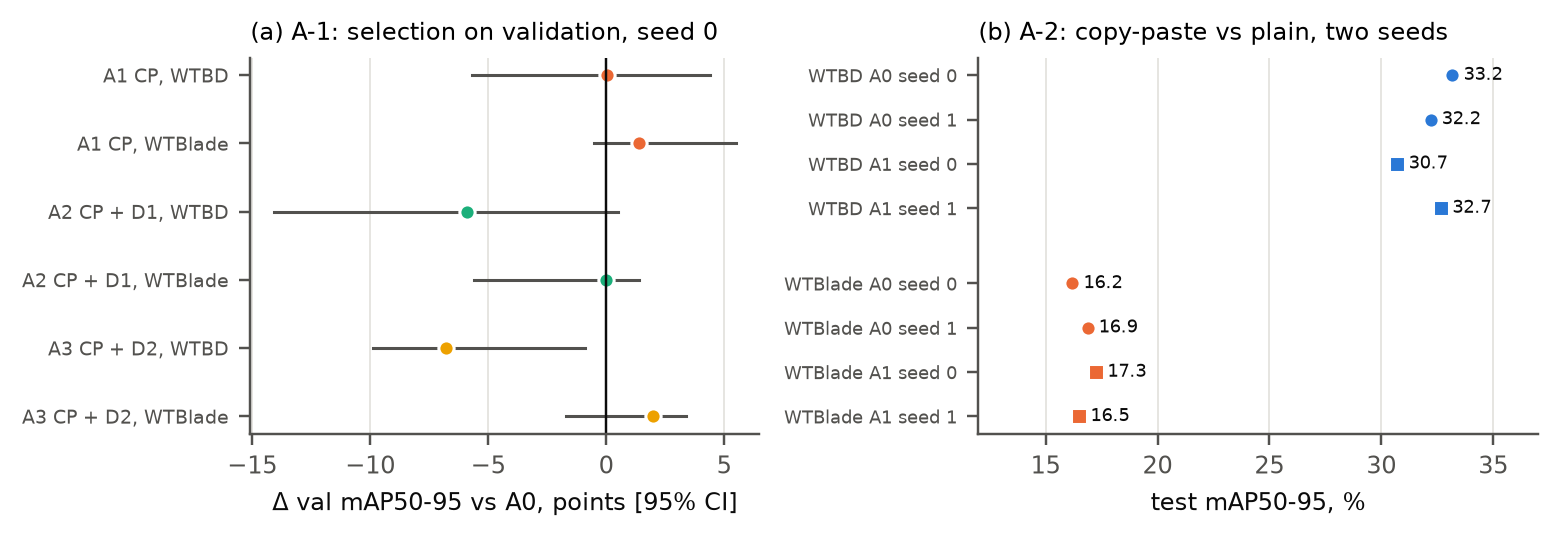
\includegraphics[width=0.94\linewidth,height=\textheight,keepaspectratio,alt={Figure 26. G27. (a) A-1, validation deltas against A0, seed 0. (b) A-2, test by seed: the seed swing is as large as the effect.}]{figures/fig16_g27.png}
\caption{Figure 26. G27. (a) A-1, validation deltas against A0, seed 0.
(b) A-2, test by seed: the seed swing is as large as the effect.}
\end{figure}

\begin{longtable}[]{@{}llll@{}}
\caption{Table 18. G27 A-2, R = A1 (copy-paste), R − A0, test mAP50-95,
mean of seeds 0 and 1. The primary claim fails.}\tabularnewline
\toprule\noalign{}
& R − A0 & 95\% CI & P(\textgreater{} 0) \\
\midrule\noalign{}
\endfirsthead
\toprule\noalign{}
& R − A0 & 95\% CI & P(\textgreater{} 0) \\
\midrule\noalign{}
\endhead
\bottomrule\noalign{}
\endlastfoot
WTBD-group & −0.99 & {[}−8.6, +1.2{]} & 0.193 \\
WTBlade-group & +0.35 & {[}−0.5, +1.6{]} & 0.812 \\
mean over datasets & −0.32 & {[}−4.1, +0.9{]} & 0.290 \\
\end{longtable}

As pre-registered, we also score without the residual pixel-twin images:
R − A0 is −1.01 on WTBD-group and +0.40 on WTBlade-group, so the
conclusion is unchanged.

R = A1 was chosen by +0.04 points on WTBD-group validation, smaller than
A0's own seed-to-seed difference on validation. D1 and D2 were rejected
on A-1 (−5.9 and −6.8 points against A1 on WTBD val), and a post hoc
check found D1 halved the encoder's last-stage effective rank (257 to
135), partial dimensional collapse. A seed swing of up to 2 points on
these test sets (A1 on WTBD: 30.7, 32.7) sets the smallest effect that
can be claimed.

Table~19 gives the validation scores that made the selection, with the
test scores beside them.

\begin{longtable}[]{@{}
  >{\raggedright\arraybackslash}p{(\linewidth - 8\tabcolsep) * \real{0.2000}}
  >{\raggedright\arraybackslash}p{(\linewidth - 8\tabcolsep) * \real{0.2000}}
  >{\raggedright\arraybackslash}p{(\linewidth - 8\tabcolsep) * \real{0.2000}}
  >{\raggedright\arraybackslash}p{(\linewidth - 8\tabcolsep) * \real{0.2000}}
  >{\raggedright\arraybackslash}p{(\linewidth - 8\tabcolsep) * \real{0.2000}}@{}}
\caption{Table 19. All G27 arms, mAP50-95 from the G27 scorer.
Validation decided R; test was not used for selection.}\tabularnewline
\toprule\noalign{}
\begin{minipage}[b]{\linewidth}\raggedright
arm
\end{minipage} & \begin{minipage}[b]{\linewidth}\raggedright
WTBD-group val, seed 0
\end{minipage} & \begin{minipage}[b]{\linewidth}\raggedright
WTBD-group test, seeds 0 / 1
\end{minipage} & \begin{minipage}[b]{\linewidth}\raggedright
WTBlade-group val, seed 0
\end{minipage} & \begin{minipage}[b]{\linewidth}\raggedright
WTBlade-group test, seeds 0 / 1
\end{minipage} \\
\midrule\noalign{}
\endfirsthead
\toprule\noalign{}
\begin{minipage}[b]{\linewidth}\raggedright
arm
\end{minipage} & \begin{minipage}[b]{\linewidth}\raggedright
WTBD-group val, seed 0
\end{minipage} & \begin{minipage}[b]{\linewidth}\raggedright
WTBD-group test, seeds 0 / 1
\end{minipage} & \begin{minipage}[b]{\linewidth}\raggedright
WTBlade-group val, seed 0
\end{minipage} & \begin{minipage}[b]{\linewidth}\raggedright
WTBlade-group test, seeds 0 / 1
\end{minipage} \\
\midrule\noalign{}
\endhead
\bottomrule\noalign{}
\endlastfoot
A0 plain & 40.11 & 33.2 / 32.2 & 15.68 & 16.2 / 16.9 \\
A1 + CP & 40.15 & 30.7 / 32.7 & 17.10 & 17.3 / 16.5 \\
A2 + CP + D1 & 34.2 & 27.4 / -- & 15.6 & 16.1 / -- \\
A3 + CP + D2 & 33.4 & 33.2 / -- & 17.7 & 16.6 / -- \\
\end{longtable}

\subsection{Semi-supervised learning in
detail}\label{semi-supervised-learning-in-detail}

Label budgets suggested semi-supervision, and it took three rounds to
rule out (Table~20). Seed noise alone is ±2.6 mAP50 at 25\%, as wide as
every effect measured. The class-balanced variant is significantly
worse, partly through a confirmation-bias runaway: one seed produced up
to about 2,300 pseudo-boxes per epoch from 24 images. Measured against
hidden labels, even a good teacher's pseudo-labels are 66\% correct at
threshold 0.5 and 40\% at 0.25.

\begin{longtable}[]{@{}
  >{\raggedright\arraybackslash}p{(\linewidth - 6\tabcolsep) * \real{0.2500}}
  >{\raggedright\arraybackslash}p{(\linewidth - 6\tabcolsep) * \real{0.2500}}
  >{\raggedright\arraybackslash}p{(\linewidth - 6\tabcolsep) * \real{0.2500}}
  >{\raggedright\arraybackslash}p{(\linewidth - 6\tabcolsep) * \real{0.2500}}@{}}
\caption{Table 20. Teacher--student rounds at 25\% of WTBD-group
{[}\citeproc{ref-meanteacher}{44}{]}. Top: one seed per arm, COCO-style
evaluator. Bottom: three seeds per arm.}\tabularnewline
\toprule\noalign{}
\begin{minipage}[b]{\linewidth}\raggedright
arm
\end{minipage} & \begin{minipage}[b]{\linewidth}\raggedright
test mAP50 / mAP50-95
\end{minipage} & \begin{minipage}[b]{\linewidth}\raggedright
val best mAP50 / mAP50-95
\end{minipage} & \begin{minipage}[b]{\linewidth}\raggedright
pseudo-labels
\end{minipage} \\
\midrule\noalign{}
\endfirsthead
\toprule\noalign{}
\begin{minipage}[b]{\linewidth}\raggedright
arm
\end{minipage} & \begin{minipage}[b]{\linewidth}\raggedright
test mAP50 / mAP50-95
\end{minipage} & \begin{minipage}[b]{\linewidth}\raggedright
val best mAP50 / mAP50-95
\end{minipage} & \begin{minipage}[b]{\linewidth}\raggedright
pseudo-labels
\end{minipage} \\
\midrule\noalign{}
\endhead
\bottomrule\noalign{}
\endlastfoot
supervised & 23.2 / 8.2 & 44.4 / 22.6 & -- \\
synthetic views, unlabelled pool & 22.4 / 7.8 & 44.8 / 22.0 & 2,748 \\
real views, unlabelled pool & 19.2 / 7.7 & 38.2 / 18.4 & 961 \\
in-domain (the rest of train, labels hidden) & 20.9 / 8.0 & 45.7 / 22.7
& 1,294 \\
supervised, 3 seeds & 21.3 ± 2.6 / 7.9 ± 1.0 & & -- \\
class-balanced in-domain, 3 seeds & 16.3 ± 2.0 / 6.6 ± 0.6 & & 5,957,
28,742, 4,372 \\
\end{longtable}

\subsection{The ledger}\label{the-ledger}

Table~21 lists the method hypotheses we ran or formally gated, with
their results. Fig.~27 plots those with a test effect in points. Some
effects are real but narrow (copy-paste on rare classes in a low-label
setting), and few survive a second dataset or a replication.

\begin{figure}
\centering
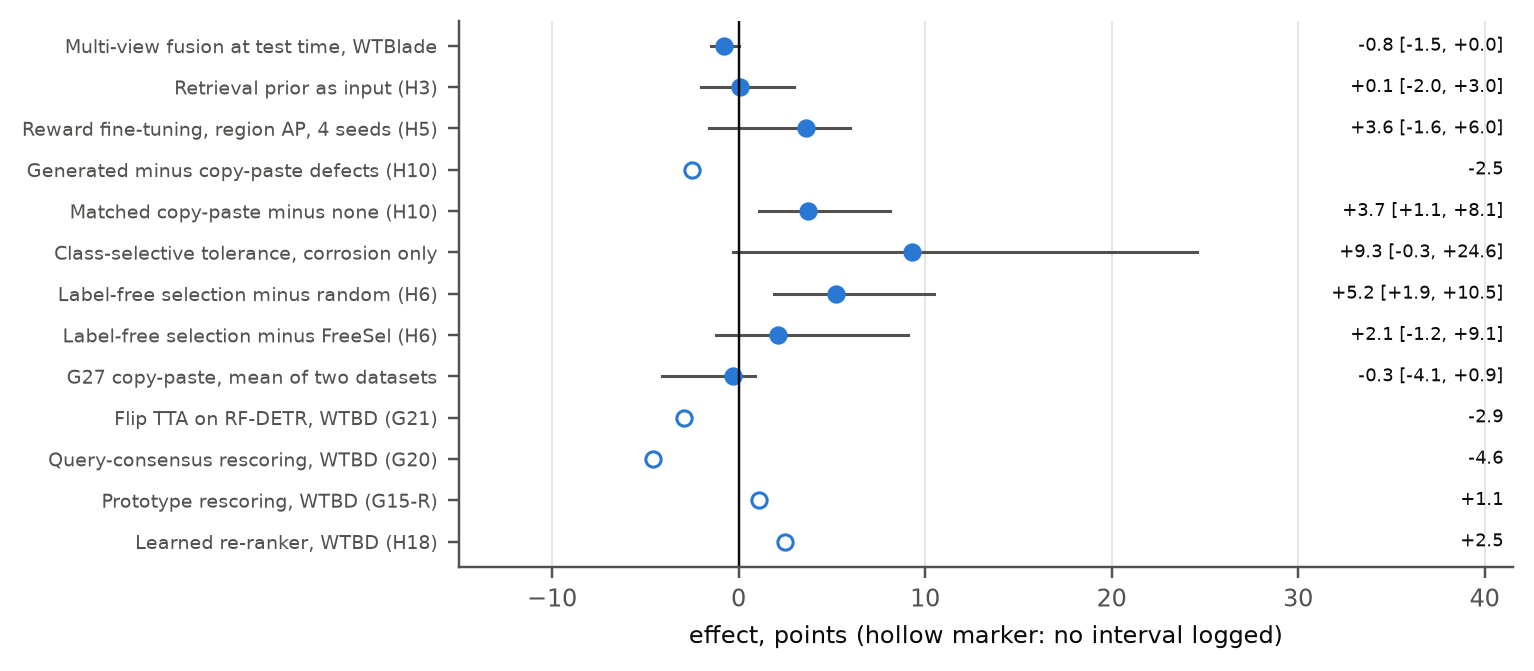
\includegraphics[width=0.9\linewidth,height=\textheight,keepaspectratio,alt={Figure 27. Effects of method tests on leak-free test sets, in points of mAP50-95 unless the ledger says otherwise. WTBD-group unless labelled. Hollow markers: no interval was logged in that form.}]{figures/fig22_failed_tests.png}
\caption{Figure 27. Effects of method tests on leak-free test sets, in
points of mAP50-95 unless the ledger says otherwise. WTBD-group unless
labelled. Hollow markers: no interval was logged in that form.}
\end{figure}

\begin{longtable}[]{@{}
  >{\raggedright\arraybackslash}p{(\linewidth - 6\tabcolsep) * \real{0.2500}}
  >{\raggedright\arraybackslash}p{(\linewidth - 6\tabcolsep) * \real{0.2500}}
  >{\raggedright\arraybackslash}p{(\linewidth - 6\tabcolsep) * \real{0.2500}}
  >{\raggedright\arraybackslash}p{(\linewidth - 6\tabcolsep) * \real{0.2500}}@{}}
\caption{Table 21. Ledger of method tests and diagnostics. WTBD-group,
test mAP50-95 points unless noted. Pre-registered from late October;
earlier rounds were decided in advance but not formally
committed.}\tabularnewline
\toprule\noalign{}
\begin{minipage}[b]{\linewidth}\raggedright
test
\end{minipage} & \begin{minipage}[b]{\linewidth}\raggedright
idea
\end{minipage} & \begin{minipage}[b]{\linewidth}\raggedright
result
\end{minipage} & \begin{minipage}[b]{\linewidth}\raggedright
verdict
\end{minipage} \\
\midrule\noalign{}
\endfirsthead
\toprule\noalign{}
\begin{minipage}[b]{\linewidth}\raggedright
test
\end{minipage} & \begin{minipage}[b]{\linewidth}\raggedright
idea
\end{minipage} & \begin{minipage}[b]{\linewidth}\raggedright
result
\end{minipage} & \begin{minipage}[b]{\linewidth}\raggedright
verdict
\end{minipage} \\
\midrule\noalign{}
\endhead
\bottomrule\noalign{}
\endlastfoot
Phases 22--24 & Teacher--student with synthetic or real views,
in-domain, class-balanced {[}\citeproc{ref-meanteacher}{44}{]}; 3 seeds
& balanced in-domain 6.6 vs supervised 7.9; mAP50 −4.2 {[}−12.1,
−0.3{]}; confirmation-bias runaway on one seed & fails \\
Phase 24 & SAM 2.1 box refinement {[}\citeproc{ref-sam2}{43}{]} & +0.3
to +0.5 at 25\%, −0.2 at 100\% & fails \\
Phases 18, 26 & Split-tolerant training; class-selective version, 2
seeds & blanket not an improvement; corrosion +9.3 {[}−0.3, +24.6{]},
mean −0.4 & targeted only \\
H1 & Multi-view fusion at test time & not testable on WTBD (26 images
with a second view); WTBlade-group −0.8 {[}−1.5, 0.0{]} & fails \\
H2 & Normal-blade anomaly prior & most anomalous patches not on defects;
box recall below chance & fails \\
H3 & Retrieval prior as a detector input & +0.1 {[}−2.0, +3.0{]} &
fails \\
H4 & Test-time adaptation across real views & gate failed: real views do
not make better detections & not run \\
H5 & Reward fine-tuning, granularity-invariant reward; 4 seeds + WTBlade
& region AP +3.6 {[}−1.6, +6.0{]}, P 0.896; WTBlade −0.6 & fails on
replication \\
H6 & Label-free scene selection by patch coverage & +5.2 {[}+1.9,
+10.5{]} over random; +2.1 {[}−1.2, +9.1{]} over FreeSel & no gain over
prior art \\
H7 & Label-free property predicting subset quality & no property
survives correction & fails \\
H8, H9 (G8, G9) & Feature upsampling; high-frequency cues & −5.9; −0.1
(mean AP) & fail \\
H10 & Generated rare-class defects vs matched copy-paste & synth − paste
−2.5; paste − none +3.7 {[}+1.1, +8.1{]} & generation fails; copy-paste
helps here \\
H12 & DINOv3 reduces subset luck & it does not; draw quality carries
over (ρ 0.71) & fails \\
G15, G15-R & Prototype rescoring & WTBD +1.1; WTBlade −0.7 & fails bar;
prior art \\
G16, G16-R & Instance-level proximity law; explains subset luck? & law
holds at instance level; does not explain subset luck; on RF-DETR it
holds for confidence, not for detection & partial \\
H16b & Deployment-targeted scene selection & gate failed & not run \\
G17 & Clicks as pseudo-boxes (bar: 60\% at IoU ≥ 0.5) & 42.0\% &
fails \\
H18, -R, -W & Learned coverage-aware re-ranker on RF-DETR & WTBD +2.5,
replicated on new models; WTBlade +0.2 & WTBD only \\
H19-W & Rescoring at the low-count boundary, WTBlade 8\% & −0.2 {[}−1.3,
+0.7{]}, P 0.286 & fails \\
G20 & Query-consensus rescoring & −4.6 WTBD; −2.1 WTBlade & fails \\
G21 & Flip agreement; plain flip TTA on RF-DETR & −2.9 WTBD; −0.6
WTBlade & fails; TTA hurts this DETR \\
G22, -O & Fine-tuning moves proximity from recall to ranking &
controlled confirmation on WTBD; not on WTBlade; holds only for
generic-feature proximity & does not replicate \\
H20 & Subset luck as annotation-convention match & no relation &
fails \\
G24 & Input resolution 768 vs 576 & WTBD +1.0 (P 0.958); WTBlade −0.1 &
dataset-specific \\
V1 & RF-DETR replaces the frozen-feature detector at 25\% & +7.3
{[}+2.3, +11.9{]}; +8.3 {[}+4.5, +15.0{]} & passes \\
Box extent; crop re-classifier & Better box refinement; re-classifying
RF-DETR candidates & prior-art and ceiling checks show little room &
discarded before any run \\
G25, G26 & Official-protocol benchmark; tuned recipe & Table~2, Table~5
& reported \\
G27 & CP, D1, D2 recipe & A-2 −0.32, P 0.290 & fails \\
G28 & Leave-one-dataset-out & dead on both targets & fails \\
\end{longtable}

\section{A cautionary history: how our own numbers were
wrong}\label{sec:history}

We report this because the same traps face anyone working on these
datasets. Fig.~28 gives the sequence, and Table~22 the original runs.

\begin{figure}
\centering
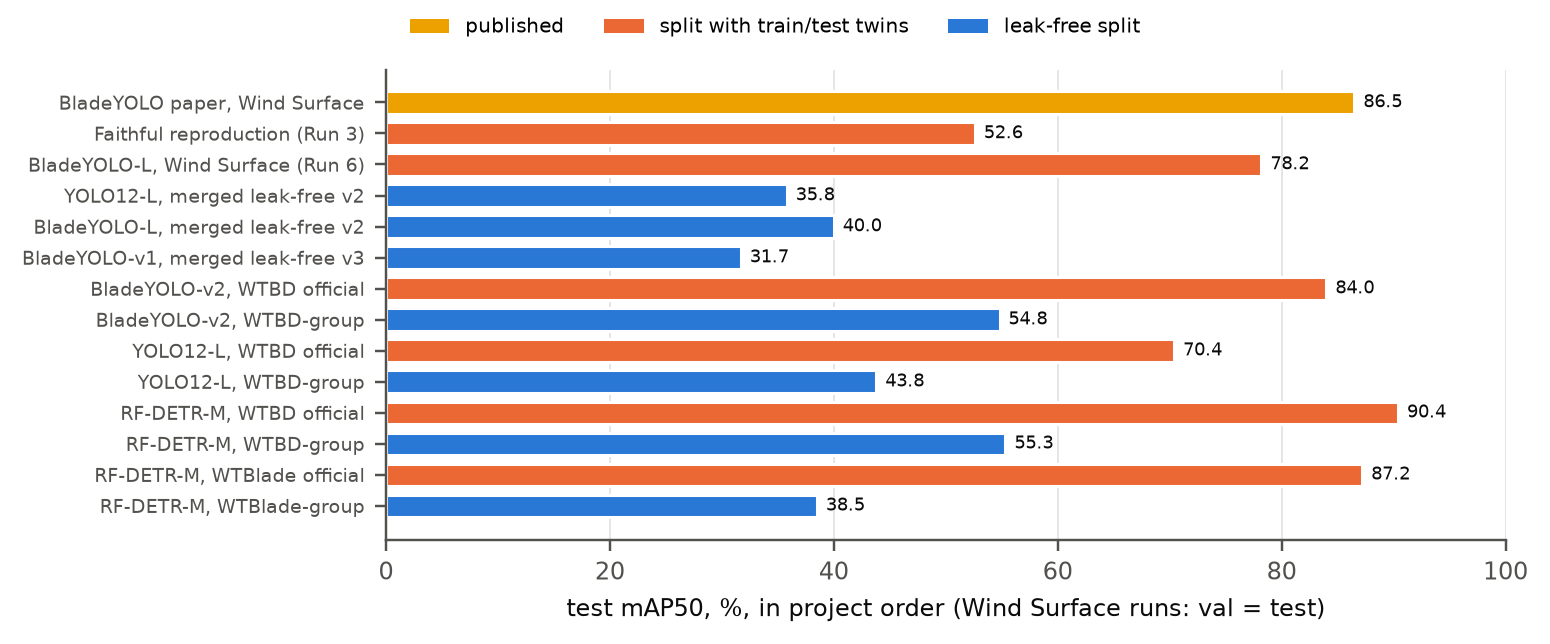
\includegraphics[width=0.92\linewidth,height=\textheight,keepaspectratio,alt={Figure 28. Reported mAP50 at each stage of the project, in order. Every class-aware score above about 60 in this figure was measured on a split with train/test twins, including our own. Datasets differ between rows, so rows are not comparable as models; the point is the pattern.}]{figures/fig23_score_history.png}
\caption{Figure 28. Reported mAP50 at each stage of the project, in
order. Every class-aware score above about 60 in this figure was
measured on a split with train/test twins, including our own. Datasets
differ between rows, so rows are not comparable as models; the point is
the pattern.}
\end{figure}

\begin{longtable}[]{@{}
  >{\raggedright\arraybackslash}p{(\linewidth - 10\tabcolsep) * \real{0.1667}}
  >{\raggedright\arraybackslash}p{(\linewidth - 10\tabcolsep) * \real{0.1667}}
  >{\raggedright\arraybackslash}p{(\linewidth - 10\tabcolsep) * \real{0.1667}}
  >{\raggedright\arraybackslash}p{(\linewidth - 10\tabcolsep) * \real{0.1667}}
  >{\raggedright\arraybackslash}p{(\linewidth - 10\tabcolsep) * \real{0.1667}}
  >{\raggedright\arraybackslash}p{(\linewidth - 10\tabcolsep) * \real{0.1667}}@{}}
\caption{Table 22. Early runs on the original Wind Surface split (2,856
train / 714 val). Later analysis invalidated the conclusions drawn from
them.}\tabularnewline
\toprule\noalign{}
\begin{minipage}[b]{\linewidth}\raggedright
run
\end{minipage} & \begin{minipage}[b]{\linewidth}\raggedright
architecture
\end{minipage} & \begin{minipage}[b]{\linewidth}\raggedright
epochs
\end{minipage} & \begin{minipage}[b]{\linewidth}\raggedright
mAP50
\end{minipage} & \begin{minipage}[b]{\linewidth}\raggedright
mAP50-95
\end{minipage} & \begin{minipage}[b]{\linewidth}\raggedright
outcome
\end{minipage} \\
\midrule\noalign{}
\endfirsthead
\toprule\noalign{}
\begin{minipage}[b]{\linewidth}\raggedright
run
\end{minipage} & \begin{minipage}[b]{\linewidth}\raggedright
architecture
\end{minipage} & \begin{minipage}[b]{\linewidth}\raggedright
epochs
\end{minipage} & \begin{minipage}[b]{\linewidth}\raggedright
mAP50
\end{minipage} & \begin{minipage}[b]{\linewidth}\raggedright
mAP50-95
\end{minipage} & \begin{minipage}[b]{\linewidth}\raggedright
outcome
\end{minipage} \\
\midrule\noalign{}
\endhead
\bottomrule\noalign{}
\endlastfoot
1--2 & paper-faithful: DINOv3 + Style Injection + WTConv + Cross-Mamba &
crash, \textasciitilde200 & & & bf16, unfreezing and DDP failures; NaN
from FFT gradients \\
3 & paper-faithful, FFT detached, SGD & \textasciitilde283 &
\textasciitilde52.6 & \textasciitilde28 & stagnated; closest
reproduction \\
4 & BladeYOLO-S (8 M parameters) & 400 & 64.3 & 37.3 & apparent ceiling
at about 64 \\
6 & BladeYOLO-L (57.2 M), AdamW & 400 & 78.2 & 46.9 & looked like a
breakthrough \\
7 & Run 6 + ``Cross-Scale Vision Mamba'' + WIoU v3 & 400 & 77.0 & 47.8 &
``+0.9 from WIoU'' \\
\end{longtable}

The gap of 33.9 / 29.4 points between Run 3 and the published 86.5 /
57.4 is far beyond run-to-run variance. These runs used a weakened
feature extractor (below) and the leaky split, so they support ``not
reproducible from the published information'', and not ``the published
modules do not work''. The paper reports 3,790 images while the public
copy has 3,570, and gives no split seed, image list or code.

\textbf{Then we audited our own code.} Run 7 was not the model we
described:

\begin{itemize}
\tightlist
\item
  \textbf{WIoU never ran}, because the patch reached the wrong
  namespace, so Run 7 trained with CIoU. Its ``+0.9 mAP50-95 from WIoU''
  was invalid. The formula also had three errors.
\item
  \textbf{The ``Mamba'' block did not perform a selective scan.} It was
  replaced by a four-direction implementation that matches a reference
  recurrence to 1.8e-14.
\item
  \textbf{The DINOv3 extractor skipped RoPE and fed unnormalised
  pixels}, so every run before 9 October used weakened features.
\item
  \textbf{The wavelet branch discarded high-frequency detail.}
\end{itemize}

\textbf{Then we found the leak.} Removing it took the numbers from about
78 to about 36--40 on a merged, deduplicated dataset (v2, 2,606 unique
images from 11,681), and a larger taxonomy-mapped v3 (5,777 images)
scored only 26--32. An exhaustive label review of 763 candidates was
worth only +3 mAP50 points. v3's limit was structural: its classes rest
on few independent scenes, and one had a single training group. Only
then did the audit lead us to WTBD alone, with its native classes.

Table~23 in the appendix lists all conclusions we later corrected.
Several were our own favourite explanations.

\section{Recommendations}\label{recommendations}

\begin{enumerate}
\def\labelenumi{\arabic{enumi}.}
\tightlist
\item
  \textbf{Split by scene, and deduplicate before augmenting.} Never
  augment before a split. Group by source photo, video and tile, and add
  a pixel test: retrieval and keypoints alone missed photometric copies
  in our own splits.
\item
  \textbf{Publish image lists}, not just ratios. The BladeYOLO
  0.87-ratio question cannot be settled without one.
\item
  \textbf{Report a leaked / no-twin breakdown} for any dataset with
  known copies. It takes minutes with cached predictions, and our tools
  are public.
\item
  \textbf{Do not tune on a leaky test set.} On these splits tuning
  measurably moved scores towards memorisation. Tune on a
  scene-separated validation set.
\item
  \textbf{Use scene-level intervals.} A 161-image test set with 58
  scenes, and some classes in fewer than 3 scenes, cannot support
  per-class claims.
\item
  \textbf{Report several labelled subsets for low-label claims.} A
  factor of two between random draws is larger than any model effect we
  saw.
\item
  \textbf{Report seeds.} On these test sets, seed swings of up to 2
  mAP50-95 points match the size of most claimed gains.
\item
  \textbf{Calibrate on unseen scenes.} A recall guarantee calibrated on
  seen scenes does not hold in the field.
\item
  \textbf{Report a granularity-invariant score beside box AP} for
  amorphous defects, and measure label self-consistency where copies
  exist.
\item
  \textbf{Test every method on a second dataset.} Several of our effects
  held on WTBD and vanished on WTBlade, and vice versa.
\item
  \textbf{Check licences at the source}, since export pages can misstate
  them.
\end{enumerate}

\section{Limitations}\label{sec:limits}

\begin{itemize}
\tightlist
\item
  \textbf{Single wind farm per dataset; small test sets} (58 and 177
  test scenes). Our leak-free numbers carry wide intervals.
\item
  \textbf{Official-protocol runs are single seed}, and their intervals
  are image-level.
\item
  \textbf{The tuning analysis is post hoc and covers one step}, with
  epochs confounded on two of three protocols.
\item
  \textbf{Wind Surface's ``no twin'' subset is not leak-free} (it shares
  drone photos with train), and WTBD's has too few boxes of three
  classes.
\item
  \textbf{WTBlade-group frames retain Roboflow's offline augmentation.}
  We keep one copy per source, so some test frames are rotated or have
  black cutouts (Fig.~24). This is a remaining difference from clean
  imagery, not a leak.
\item
  \textbf{YOLO12-L on WTBlade-group may be under-trained:} 50 epochs,
  the budget planned for BladeYOLO-v2 ViT-B on this set, with its best
  validation at epoch 43 after a nearly linear rise. Its 13.3 may
  understate it.
\item
  \textbf{Our leak-free splits have a small residual leak} (§~4,
  Fig.~5): under a point on WTBD-group, negligible on WTBlade-group.
  G28's ID arm benefits from it slightly.
\item
  \textbf{G27 A-2 uses two seeds; G28 uses one.} G28 X arms train for 12
  epochs, as G27's stage 1, at 640 px. X-WTBlade loses the largest
  source, and its pool is 45\% smaller than X-WTBD's, which may
  contribute to the difference between targets.
\item
  \textbf{Hardware differs between seeds.} G27 seed 0 ran on Kaggle
  (fp16) and seed 1 on an A100 (bf16). Arms are paired within a seed,
  but the seed effect includes hardware. An earlier A0 seed-1 run on
  Kaggle scored 31.2 on WTBD-group test against 32.2 on the A100.
\item
  \textbf{Region AP depends on defect size.} A trivial whole-image
  detector scores 14--24 here, so raw region AP must be read against
  that floor.
\item
  \textbf{Claims about modules are for our components.} BladeYOLO's own
  modules were not rerun on a leak-free split after the code audit.
\item
  \textbf{Deviations from pre-registration.} The G26 rule formally
  selected RF-DETR-L (validation 63.4 against 62.0), which lost on test
  (−1.7), and we did not run L on the other protocols; this cannot
  inflate a reported number, but it is a deviation. G27's phase B on the
  official protocols was not run, since the recipe failed A-2.
\item
  \textbf{The literature check is not exhaustive}, and ``new for this
  domain'' means that we did not find an earlier audit.
\end{itemize}

\section{Data and code availability}\label{sec:availability}

\textbf{Code and records.} All code, tests, split files, per-image flags
and the full research log (\texttt{research\_log.md}) are at
\url{https://github.com/bhavya-goel-11/BladeYOLO}. To regenerate this
paper's numbers and figures, run \texttt{tools/official\_leak\_eval.py},
\texttt{tools/g27\_score.py}, \texttt{tools/g28\_score.py},
\texttt{tools/paper\_evidence.py}, \texttt{tools/paper\_figures.py},
\texttt{tools/paper\_figures2.py} and \texttt{tools/build\_paper.py}.
The training queue is \texttt{tools/sessions.sh}.

\textbf{Data.} The datasets, leak-free splits and pools are assembled as
\texttt{blade-defect-benchmark}, with per-folder licences in its
\texttt{LICENSES.md}. WTBD is CC BY 4.0. WTBlade-Defect contains DTU
NordTank images {[}\citeproc{ref-shihavuddin}{5}{]} under CC BY-NC,
despite its Roboflow page, and derived folders inherit this, so they are
for non-commercial research only. The Wind Surface licence is unclear
from its source. Images in our figures are shown for scientific comment;
sources are cited above.

\textbf{Foundation models.} We acknowledge DINOv3
{[}\citeproc{ref-dinov3}{21}{]}, used under the DINOv3 License, and
DINOv2 {[}\citeproc{ref-dinov2}{19}{]} through RF-DETR
{[}\citeproc{ref-rfdetr}{18}{]}. Trained checkpoints containing DINOv3
weights must ship with that licence.

\section*{Appendix}\label{appendix}
\addcontentsline{toc}{section}{Appendix}

\subsection*{A. Corrections to our own
conclusions}\label{a.-corrections-to-our-own-conclusions}
\addcontentsline{toc}{subsection}{A. Corrections to our own conclusions}

\begin{longtable}[]{@{}
  >{\raggedright\arraybackslash}p{(\linewidth - 4\tabcolsep) * \real{0.3333}}
  >{\raggedright\arraybackslash}p{(\linewidth - 4\tabcolsep) * \real{0.3333}}
  >{\raggedright\arraybackslash}p{(\linewidth - 4\tabcolsep) * \real{0.3333}}@{}}
\caption{Table 23. Conclusions we later corrected. Kept here because
each was plausible at the time.}\tabularnewline
\toprule\noalign{}
\begin{minipage}[b]{\linewidth}\raggedright
earlier conclusion
\end{minipage} & \begin{minipage}[b]{\linewidth}\raggedright
status
\end{minipage} & \begin{minipage}[b]{\linewidth}\raggedright
why
\end{minipage} \\
\midrule\noalign{}
\endfirsthead
\toprule\noalign{}
\begin{minipage}[b]{\linewidth}\raggedright
earlier conclusion
\end{minipage} & \begin{minipage}[b]{\linewidth}\raggedright
status
\end{minipage} & \begin{minipage}[b]{\linewidth}\raggedright
why
\end{minipage} \\
\midrule\noalign{}
\endhead
\bottomrule\noalign{}
\endlastfoot
Runs 6--7 reach \textasciitilde78 / \textasciitilde47 on Wind Surface &
invalid & 75\% of validation had train twins (first count) \\
WIoU v3 gave +0.9 mAP50-95 & invalid & never active; Run 7 trained with
CIoU \\
Mamba added global context & invalid & the block did not scan \\
SGD → AdamW was the breakthrough & confounded & changed together with an
8 M → 57 M scale-up \\
The remaining gap is locality bias & superseded & the gap was leakage
and data structure \\
v3 is better because it is larger & superseded & scenes matter, not
files (Wind Surface 81; WTBD 550) \\
Mislabelling explains poor v3 scores & rejected & the review was worth
only +3 mAP50 points \\
BladeYOLO-v2's win shows the architecture generalises & qualified & it
rests mainly on thunderstrike (3 test scenes) \\
The advantage comes from the architecture & rejected & the frozen DINOv3
features carry it all \\
Honest calibration costs 2.4 vs 1.0 false alarms per image & corrected &
that column counted all predictions; real false alarms 0.2 vs 0.1 \\
WTBD copies agree on 86.0\% & refined & rotated copies inflate
``loose''; axis-aligned 87.3\% \\
Part of the inflation is memorised box splitting & not supported &
tolerant gain is not smaller on images with a twin \\
At 25\%, most lost defects are found but boxed differently & refined &
near-misses (34--36\%) and misses (19--27\%) are of similar size \\
Split tolerance helps corrosion & replicated, not significant & +9.3
{[}−0.3, +24.6{]}; aggregate unchanged \\
The DINOv3 advantage is a low-data advantage & corrected & absolute gain
does not shrink with data \\
The gain grows with frozen backbone size & partly supported & ViT-B
beats ViT-S; ViT-L does not beat ViT-B \\
Teacher--student gives a small consistent gain & qualified & seed noise
was as large; balanced variant significantly worse \\
Leak-free mAP50-95 / mAP50 ratios are 0.42--0.47 & corrected &
full-label RF-DETR on WTBD-group reaches 0.60 \\
\end{longtable}

\subsection*{B. Engineering problems that affected
results}\label{b.-engineering-problems-that-affected-results}
\addcontentsline{toc}{subsection}{B. Engineering problems that affected
results}

\begin{longtable}[]{@{}
  >{\raggedright\arraybackslash}p{(\linewidth - 4\tabcolsep) * \real{0.3333}}
  >{\raggedright\arraybackslash}p{(\linewidth - 4\tabcolsep) * \real{0.3333}}
  >{\raggedright\arraybackslash}p{(\linewidth - 4\tabcolsep) * \real{0.3333}}@{}}
\caption{Table 24. Defects we found and fixed. Several of them silently
changed what was being measured. Mixed-precision overflow was the most
frequent.}\tabularnewline
\toprule\noalign{}
\begin{minipage}[b]{\linewidth}\raggedright
problem
\end{minipage} & \begin{minipage}[b]{\linewidth}\raggedright
root cause
\end{minipage} & \begin{minipage}[b]{\linewidth}\raggedright
fix
\end{minipage} \\
\midrule\noalign{}
\endfirsthead
\toprule\noalign{}
\begin{minipage}[b]{\linewidth}\raggedright
problem
\end{minipage} & \begin{minipage}[b]{\linewidth}\raggedright
root cause
\end{minipage} & \begin{minipage}[b]{\linewidth}\raggedright
fix
\end{minipage} \\
\midrule\noalign{}
\endhead
\bottomrule\noalign{}
\endlastfoot
WIoU never active & patched the wrong namespace & patch the loss
namespace \\
NaN in selective scan (epoch 9) & fp16 overflow before LayerNorm & fp32
LayerNorm \\
NaN at epoch 4 & poisoned WIoU running mean; aggressive warm-up &
finite-only mean; lr 0.001, bias warm-up 0 \\
NaN at epoch 17 & fp16 overflow from a conv into BN & fp32 blocks for
refinement \\
NaN at epoch 99, validation at 0 & NaN batch poisons BN statistics and
EMA & per-batch BN repair and step skip, reported \\
NaN late in training (epochs 99--149) & YOLOv12 area attention forms
scores in fp16 (\textasciitilde4e5, above the fp16 maximum) & scores and
softmax in fp32 \\
Test metrics silently missing & \texttt{deform\_conv2d} segfault on NaN
offsets from the FLOPs probe's uninitialised image & finite, clamped
offsets; test in a fresh process \\
Silent resume from an old checkpoint & training script reused any
\texttt{last.pt} & explicit \texttt{-\/-resume} \\
RF-DETR learning rate never decayed & default step at epoch 100 never
fires & explicit cosine schedule (G26) \\
Scorer read a stale result after a time-out & an earlier output file had
the same name & rerun with no limit; check file freshness \\
\end{longtable}

\subsection*{C. Notation and experiment
names}\label{c.-notation-and-experiment-names}
\addcontentsline{toc}{subsection}{C. Notation and experiment names}

Names follow the research log: H\emph{n} and G\emph{n} are hypotheses
and gates in order of registration. A0--A3 are the G27 arms: A0 plain
recipe, A1 + copy-paste, A2 + copy-paste + D1, A3 + copy-paste + D2. ID
and X are the G28 arms. ``Points'' are percentage points of AP.
WTBD-official is WTBD's own split.

\subsection*{D. Per-class audit}\label{d.-per-class-audit}
\addcontentsline{toc}{subsection}{D. Per-class audit}

\begin{longtable}[]{@{}
  >{\raggedright\arraybackslash}p{(\linewidth - 16\tabcolsep) * \real{0.1111}}
  >{\raggedright\arraybackslash}p{(\linewidth - 16\tabcolsep) * \real{0.1111}}
  >{\raggedright\arraybackslash}p{(\linewidth - 16\tabcolsep) * \real{0.1111}}
  >{\raggedright\arraybackslash}p{(\linewidth - 16\tabcolsep) * \real{0.1111}}
  >{\raggedright\arraybackslash}p{(\linewidth - 16\tabcolsep) * \real{0.1111}}
  >{\raggedright\arraybackslash}p{(\linewidth - 16\tabcolsep) * \real{0.1111}}
  >{\raggedright\arraybackslash}p{(\linewidth - 16\tabcolsep) * \real{0.1111}}
  >{\raggedright\arraybackslash}p{(\linewidth - 16\tabcolsep) * \real{0.1111}}
  >{\raggedright\arraybackslash}p{(\linewidth - 16\tabcolsep) * \real{0.1111}}@{}}
\caption{Table 25. Content audit by native class
(\texttt{runs/analysis/datasets/report.md}). \emph{Learnable} boxes are
those kept after deduplication. \emph{Purity} is mutual crop retrieval
within the class. Median box size is in pixels at 640. The check export
of Beijing is omitted because it is the same data.}\tabularnewline
\toprule\noalign{}
\begin{minipage}[b]{\linewidth}\raggedright
dataset
\end{minipage} & \begin{minipage}[b]{\linewidth}\raggedright
class
\end{minipage} & \begin{minipage}[b]{\linewidth}\raggedright
raw images
\end{minipage} & \begin{minipage}[b]{\linewidth}\raggedright
raw boxes
\end{minipage} & \begin{minipage}[b]{\linewidth}\raggedright
unique images
\end{minipage} & \begin{minipage}[b]{\linewidth}\raggedright
scenes
\end{minipage} & \begin{minipage}[b]{\linewidth}\raggedright
learnable boxes
\end{minipage} & \begin{minipage}[b]{\linewidth}\raggedright
median box px
\end{minipage} & \begin{minipage}[b]{\linewidth}\raggedright
purity
\end{minipage} \\
\midrule\noalign{}
\endfirsthead
\toprule\noalign{}
\begin{minipage}[b]{\linewidth}\raggedright
dataset
\end{minipage} & \begin{minipage}[b]{\linewidth}\raggedright
class
\end{minipage} & \begin{minipage}[b]{\linewidth}\raggedright
raw images
\end{minipage} & \begin{minipage}[b]{\linewidth}\raggedright
raw boxes
\end{minipage} & \begin{minipage}[b]{\linewidth}\raggedright
unique images
\end{minipage} & \begin{minipage}[b]{\linewidth}\raggedright
scenes
\end{minipage} & \begin{minipage}[b]{\linewidth}\raggedright
learnable boxes
\end{minipage} & \begin{minipage}[b]{\linewidth}\raggedright
median box px
\end{minipage} & \begin{minipage}[b]{\linewidth}\raggedright
purity
\end{minipage} \\
\midrule\noalign{}
\endhead
\bottomrule\noalign{}
\endlastfoot
Wind Surface & corrosion & 660 & 2116 & 90 & 10 & 294 & 87.7 & 0.894 \\
Wind Surface & dirt & 1044 & 1067 & 487 & 14 & 488 & 257.3 & 0.923 \\
Wind Surface & hide\_craze & 1305 & 2321 & 272 & 50 & 491 & 53.6 &
0.719 \\
Wind Surface & surface\_eye & 108 & 412 & 9 & 1 & 40 & 85.5 & 0.0 \\
Wind Surface & thunderstrike & 364 & 478 & 70 & 10 & 89 & 55.5 & 0.12 \\
WTBlade & burn & 736 & 1019 & 116 & 104 & 166 & 56.9 & 0.65 \\
WTBlade & crack & 1409 & 2525 & 177 & 112 & 335 & 63.0 & 0.573 \\
WTBlade & deformity & 1801 & 2291 & 282 & 231 & 383 & 130.7 & 0.802 \\
WTBlade & dirt & 5148 & 8875 & 585 & 425 & 928 & 255.2 & 0.683 \\
WTBlade & oil & 539 & 958 & 97 & 82 & 167 & 105.6 & 0.428 \\
WTBlade & peeling & 2307 & 5715 & 172 & 80 & 395 & 96.5 & 0.583 \\
WTBlade & rust & 2043 & 4188 & 157 & 123 & 258 & 95.2 & 0.354 \\
Beijing & corrosion & 789 & 2565 & 90 & 10 & 292 & 86.9 & 0.666 \\
Beijing & craze & 57 & 69 & 9 & 8 & 12 & 158.3 & 0.108 \\
Beijing & hide\_craze & 1187 & 2137 & 283 & 52 & 499 & 54.9 & 0.545 \\
Beijing & surface\_eye & 3316 & 5489 & 900 & 17 & 1467 & 227.3 &
0.888 \\
Beijing & surface\_injure & 1662 & 3285 & 290 & 45 & 564 & 85.3 &
0.635 \\
Beijing & surface\_oil & 1588 & 2242 & 417 & 27 & 574 & 249.9 & 0.473 \\
Beijing & thunderstrike & 270 & 353 & 69 & 10 & 87 & 52.2 & 0.153 \\
WTBs2025 & oil leakage & 512 & 572 & 28 & 28 & 35 & 33.9 & 0.486 \\
WTBs2025 & paint cracks & 458 & 514 & 398 & 351 & 235 & 17.8 & 0.666 \\
WTBs2025 & localized damage & 1027 & 1254 & 773 & 655 & 86 & 6.5 &
0.256 \\
WTBs2025 & lightning strikes & 285 & 354 & 89 & 43 & 96 & 43.1 & 0.56 \\
WTBs2025 & surface stains & 263 & 294 & 226 & 211 & 142 & 23.5 &
0.182 \\
WTBs2025 & erosion & 2798 & 4517 & 1132 & 993 & 1174 & 21.4 & 0.675 \\
WTBs2025 & coating detachment & 1085 & 1906 & 703 & 566 & 526 & 15.3 &
0.484 \\
WTBs2025 & protective film damage & 546 & 632 & 393 & 350 & 195 & 14.2 &
0.639 \\
WTBs2025 & pinholes & 522 & 774 & 377 & 311 & 45 & 2.2 & 0.136 \\
WTBD & craze & 198 & 257 & 94 & 86 & 119 & 206.5 & 0.555 \\
WTBD & corrosion & 172 & 257 & 105 & 100 & 149 & 194.3 & 0.723 \\
WTBD & surface\_injure & 264 & 412 & 164 & 155 & 247 & 103.3 & 0.723 \\
WTBD & thunderstrike & 89 & 92 & 50 & 47 & 52 & 138.0 & 0.565 \\
WTBD & crack & 177 & 224 & 47 & 37 & 55 & 171.5 & 0.842 \\
WTBD & hide\_craze & 249 & 342 & 182 & 171 & 244 & 111.9 & 0.785 \\
\end{longtable}

\subsection*{E. Run registry}\label{e.-run-registry}
\addcontentsline{toc}{subsection}{E. Run registry}

\begin{longtable}[]{@{}
  >{\raggedright\arraybackslash}p{(\linewidth - 8\tabcolsep) * \real{0.2000}}
  >{\raggedright\arraybackslash}p{(\linewidth - 8\tabcolsep) * \real{0.2000}}
  >{\raggedright\arraybackslash}p{(\linewidth - 8\tabcolsep) * \real{0.2000}}
  >{\raggedright\arraybackslash}p{(\linewidth - 8\tabcolsep) * \real{0.2000}}
  >{\raggedright\arraybackslash}p{(\linewidth - 8\tabcolsep) * \real{0.2000}}@{}}
\caption{Table 26. Runs of the final phase (G27, G28, YOLO12-L). Val
best is the best EMA epoch (Ultralytics best epoch for YOLO12-L). Test
values are from Table~7 and Table~15.}\tabularnewline
\toprule\noalign{}
\begin{minipage}[b]{\linewidth}\raggedright
run
\end{minipage} & \begin{minipage}[b]{\linewidth}\raggedright
data
\end{minipage} & \begin{minipage}[b]{\linewidth}\raggedright
epochs (best)
\end{minipage} & \begin{minipage}[b]{\linewidth}\raggedright
val best mAP50 / mAP50-95
\end{minipage} & \begin{minipage}[b]{\linewidth}\raggedright
test mAP50 / mAP50-95
\end{minipage} \\
\midrule\noalign{}
\endfirsthead
\toprule\noalign{}
\begin{minipage}[b]{\linewidth}\raggedright
run
\end{minipage} & \begin{minipage}[b]{\linewidth}\raggedright
data
\end{minipage} & \begin{minipage}[b]{\linewidth}\raggedright
epochs (best)
\end{minipage} & \begin{minipage}[b]{\linewidth}\raggedright
val best mAP50 / mAP50-95
\end{minipage} & \begin{minipage}[b]{\linewidth}\raggedright
test mAP50 / mAP50-95
\end{minipage} \\
\midrule\noalign{}
\endhead
\bottomrule\noalign{}
\endlastfoot
\texttt{rfdetrm768cos\_wtbd\_group\_full} & WTBD-group, A0, s0 & 100
(20) & 64.8 / 40.4 & 55.3 / 33.2 \\
\texttt{rfdetrm768cos\_wtbd\_group\_full\_s1} & WTBD-group, A0, s1 & 100
(32) & 67.1 / 40.8 & 54.8 / 32.2 \\
\texttt{rfdetrm768cos\_cp\_wtbd\_group\_full} & WTBD-group, A1, s0 & 100
(9) & 63.9 / 40.1 & 51.5 / 30.7 \\
\texttt{rfdetrm768cos\_cp\_wtbd\_group\_full\_s1} & WTBD-group, A1, s1 &
100 (31) & 70.7 / 41.8 & 58.5 / 32.7 \\
\texttt{rfdetrm768cos\_cp\_d1\_wtbd\_group\_full} & WTBD-group, A2 & 100
(63) & 59.6 / 34.4 & 49.6 / 27.4 \\
\texttt{rfdetrm768cos\_cp\_d2\_wtbd\_group\_full} & WTBD-group, A3 & 100
(40) & 56.8 / 33.8 & 55.3 / 33.2 \\
\texttt{rfdetrm640cos\_wtblade\_group\_full} & WTBlade-group, A0, s0 &
60 (11) & 38.4 / 15.7 & 38.5 / 16.2 \\
\texttt{rfdetrm640cos\_wtblade\_group\_full\_s1} & WTBlade-group, A0, s1
& 60 (17) & 41.1 / 16.2 & 41.0 / 16.9 \\
\texttt{rfdetrm640cos\_cp\_wtblade\_group\_full} & WTBlade-group, A1, s0
& 60 (13) & 41.6 / 17.1 & 41.8 / 17.3 \\
\texttt{rfdetrm640cos\_cp\_wtblade\_group\_full\_s1} & WTBlade-group,
A1, s1 & 60 (16) & 41.3 / 16.9 & 39.3 / 16.5 \\
\texttt{rfdetrm640cos\_cp\_d1\_wtblade\_group\_full} & WTBlade-group, A2
& 60 (16) & 39.2 / 15.7 & 40.1 / 16.1 \\
\texttt{rfdetrm640cos\_cp\_d2\_wtblade\_group\_full} & WTBlade-group, A3
& 60 (8) & 44.2 / 17.8 & 41.7 / 16.6 \\
\texttt{rfdetrm640ag\_id\_wtbd\_group} & ID-WTBD, class-agnostic & 100
(23) & 80.7 / 48.3 & 72.9 / 41.9 \\
\texttt{rfdetrm640ag\_id\_wtblade\_group} & ID-WTBlade, class-agnostic &
60 (26) & 49.5 / 20.5 & 51.7 / 21.5 \\
\texttt{rfdetrm640ag\_x\_wtbd\_group} & X-WTBD, class-agnostic & 12 (12)
& 72.2 / 38.6 (own val) & 17.7 / 6.0 \\
\texttt{rfdetrm640ag\_x\_wtblade\_group} & X-WTBlade, class-agnostic &
12 (12) & 62.1 / 33.6 (own val) & 2.4 / 0.5 \\
\texttt{yolo12l\_wtblade\_group} & WTBlade-group & 50 (43) & 33.6 / 12.5
& 32.2 / 13.3 \\
\end{longtable}

\begin{longtable}[]{@{}
  >{\raggedright\arraybackslash}p{(\linewidth - 12\tabcolsep) * \real{0.1429}}
  >{\raggedright\arraybackslash}p{(\linewidth - 12\tabcolsep) * \real{0.1429}}
  >{\raggedright\arraybackslash}p{(\linewidth - 12\tabcolsep) * \real{0.1429}}
  >{\raggedright\arraybackslash}p{(\linewidth - 12\tabcolsep) * \real{0.1429}}
  >{\raggedright\arraybackslash}p{(\linewidth - 12\tabcolsep) * \real{0.1429}}
  >{\raggedright\arraybackslash}p{(\linewidth - 12\tabcolsep) * \real{0.1429}}
  >{\raggedright\arraybackslash}p{(\linewidth - 12\tabcolsep) * \real{0.1429}}@{}}
\caption{Table 27. Registry of earlier runs, as kept in the research log
(§27 there; section references inside this table are to the log). Scores
are fractions, not percent.}\tabularnewline
\toprule\noalign{}
\begin{minipage}[b]{\linewidth}\raggedright
Run folder
\end{minipage} & \begin{minipage}[b]{\linewidth}\raggedright
Data
\end{minipage} & \begin{minipage}[b]{\linewidth}\raggedright
Model
\end{minipage} & \begin{minipage}[b]{\linewidth}\raggedright
Epochs
\end{minipage} & \begin{minipage}[b]{\linewidth}\raggedright
Val best (mAP50 / 50-95)
\end{minipage} & \begin{minipage}[b]{\linewidth}\raggedright
Test (mAP50 / 50-95)
\end{minipage} & \begin{minipage}[b]{\linewidth}\raggedright
Notes
\end{minipage} \\
\midrule\noalign{}
\endfirsthead
\toprule\noalign{}
\begin{minipage}[b]{\linewidth}\raggedright
Run folder
\end{minipage} & \begin{minipage}[b]{\linewidth}\raggedright
Data
\end{minipage} & \begin{minipage}[b]{\linewidth}\raggedright
Model
\end{minipage} & \begin{minipage}[b]{\linewidth}\raggedright
Epochs
\end{minipage} & \begin{minipage}[b]{\linewidth}\raggedright
Val best (mAP50 / 50-95)
\end{minipage} & \begin{minipage}[b]{\linewidth}\raggedright
Test (mAP50 / 50-95)
\end{minipage} & \begin{minipage}[b]{\linewidth}\raggedright
Notes
\end{minipage} \\
\midrule\noalign{}
\endhead
\bottomrule\noalign{}
\endlastfoot
Runs 1--5 & WS original & Paper-faithful / BladeYOLO-S & --- & see §2 &
--- & Logs on Kaggle only \\
\texttt{bladeyolo\_l\_sota} (Run 6) & WS original (\textbf{leaky}) &
BladeYOLO-L & 400 & 0.781 / 0.469 & --- & Inflated \\
\texttt{bladeyolo\_l\_sota-2} (Run 7) & WS original (\textbf{leaky}) &
BladeYOLO-L + ``Mamba'' + (inactive) WIoU & 400 & 0.769 / 0.478 & --- &
Inflated \\
\texttt{yolo12l\_baseline} & v2 & YOLO12-L & 266 & 0.290 / 0.122 & 0.358
/ 0.149 & lr0 0.002 \\
\texttt{bladeyolo\_l} & v2 & BladeYOLO-L (repaired) & 167 (stopped) &
0.344 / 0.123 & 0.400 / 0.146 (epoch 124) & \\
\texttt{yolo12l\_v3} & v3 & YOLO12-L & 150 & 0.290 / 0.141 & 0.263 /
0.109 & Old harmful recipe \\
\texttt{bladeyolo\_v3} & v3 & BladeYOLO-L v1 & 150 & 0.356 / 0.156 &
0.317 / 0.124 & \\
\texttt{bladeyolo2\_v3} & v3 & BladeYOLO-v2 & 100 & 0.369 / 0.172 &
0.296 / 0.123 (evaluator) & Test lost on Kaggle (segfault) \\
WBF ensemble & v3 / v3.2 & 3 models & --- & --- & 0.339 / 0.143 (v3);
\textasciitilde0.411 / 0.168 (merged) & Fusion IoU chosen on val \\
\texttt{bladeyolo2\_wtbd\_group} (attempt 1) & WTBD-group & BladeYOLO-v2
& 99 of 150 & 0.649 / 0.379 & --- & NaN at epoch 99; folder lost \\
\textbf{\texttt{bladeyolo2\_wtbd\_group}} & WTBD-group (leak-free) &
BladeYOLO-v2 & 150 & 0.650 / 0.368 (epoch 124) & \textbf{0.548 / 0.245};
TTA 0.574 / 0.279 & Test run locally \\
\textbf{\texttt{bladeyolo2\_wtbd\_official}} & WTBD official
(\textbf{leaky}) & BladeYOLO-v2 & 120 & 0.845 / 0.475 (epoch 105) &
\textbf{0.840 / 0.493}; TTA 0.830 / 0.517 & TTA run locally \\
\textbf{\texttt{bladeyolo2\_wtbd\_group\_tolerant}} & WTBD-group
(leak-free) & BladeYOLO-v2, split-tolerant targets & 150 & 0.609 / 0.352
(epoch 83) & \textbf{0.523 / 0.249}; TTA 0.552 / 0.282 & 5 NaN batches
dropped (attention overflow, since fixed) \\
\texttt{bladeyolo2\_wtbd\_group\_f25} & WTBD-group, 25\% of train scenes
& BladeYOLO-v2 & 150 & 0.444 / 0.226 (epoch 126) & \textbf{0.232 /
0.082}; TTA 0.269 / 0.105 & Learning curve \\
\texttt{bladeyolo2\_wtbd\_group\_f50} & WTBD-group, 50\% of train scenes
& BladeYOLO-v2 & 150 & 0.472 / 0.263 (epoch 140) & \textbf{0.413 /
0.183}; TTA 0.473 / 0.211 & Learning curve \\
\texttt{yolo12l\_wtbd\_group\_f25} & WTBD-group, 25\% of train scenes &
YOLO12-L & 150 & 0.233 / 0.139 (epoch 150) & \textbf{0.106 / 0.037}; TTA
0.144 / 0.059 & Learning curve \\
\texttt{yolo12l\_wtbd\_group\_f50} & WTBD-group, 50\% of train scenes &
YOLO12-L & 150 & 0.279 / 0.167 (epoch 120) & \textbf{0.244 / 0.105}; TTA
0.259 / 0.125 & Learning curve \\
\texttt{bladeyolo2\_wtbd\_group\_f25\_sslsyn} & WTBD-group 25\% + view
pool & BladeYOLO-v2, synthetic-view teacher--student & 150 & 0.427 /
0.203 (epoch 142) & \textbf{0.221 / 0.071}; TTA 0.233 / 0.089 & Phase
22 \\
\texttt{bladeyolo2\_wtbd\_group\_f25\_sslreal} & WTBD-group 25\% + view
pool & BladeYOLO-v2, real-view teacher--student & 150 & 0.450 / 0.210
(epoch 107) & \textbf{0.213 / 0.085}; TTA 0.268 / 0.107 & Phase 22;
teacher collapsed \\
\texttt{bladeyolo2\_wtbd\_group\_f25\_sslsyn2} & WTBD-group 25\% + view
pool & BladeYOLO-v2, synthetic views (fixed) & 150 & 0.448 / 0.220
(epoch 122) & \textbf{0.224 / 0.078}; TTA 0.259 / 0.106 & Phase 23 \\
\texttt{bladeyolo2\_wtbd\_group\_f25\_sslreal2} & WTBD-group 25\% + view
pool & BladeYOLO-v2, real views (fixed) & 150 & 0.382 / 0.184 (epoch
127) & \textbf{0.192 / 0.077}; TTA 0.248 / 0.101 & Phase 23 \\
\texttt{bladeyolo2\_wtbd\_group\_f25\_sslin} & WTBD-group 25\% + other
75\% unlabelled & BladeYOLO-v2, in-domain teacher--student & 150 & 0.457
/ 0.227 (epoch 131) & \textbf{0.209 / 0.080}; TTA 0.245 / 0.101 & Phase
23 \\
\texttt{bladeyolo2\_wtbd\_group\_f25\_s1} & WTBD-group, 25\% of train
scenes & BladeYOLO-v2, seed 1 & 150 & 0.411 / 0.199 (epoch 129) &
\textbf{0.224 / 0.087}; TTA 0.242 / 0.105 & Phase 24 \\
\texttt{bladeyolo2\_wtbd\_group\_f25\_s2} & WTBD-group, 25\% of train
scenes & BladeYOLO-v2, seed 2 & 150 & 0.435 / 0.203 (epoch 143) &
\textbf{0.184 / 0.068}; TTA 0.229 / 0.096 & Phase 24 \\
\texttt{bladeyolo2\_wtbd\_group\_f25\_sslinb\_s0} & WTBD-group 25\% +
other 75\% unlabelled & BladeYOLO-v2, in-domain, class-balanced, seed 0
& 150 & 0.344 / 0.154 (epoch 75) & \textbf{0.143 / 0.060}; TTA 0.183 /
0.079 & Phase 24 \\
\texttt{bladeyolo2\_wtbd\_group\_f25\_sslinb\_s1} & WTBD-group 25\% +
other 75\% unlabelled & same, seed 1 & 150 & 0.352 / 0.167 (epoch 92) &
\textbf{0.163 / 0.065}; TTA 0.180 / 0.075 & Phase 24; pseudo-label
runaway, epochs 33--62 \\
\texttt{bladeyolo2\_wtbd\_group\_f25\_sslinb\_s2} & WTBD-group 25\% +
other 75\% unlabelled & same, seed 2 & 150 & 0.445 / 0.205 (epoch 148) &
\textbf{0.183 / 0.073}; TTA 0.213 / 0.095 & Phase 24 \\
\texttt{bladeyolo2nodino\_wtbd\_group\_f25\_s0} & WTBD-group, 25\% of
train scenes & BladeYOLO-v2 without DINOv3, seed 0 & 150 & 0.229 / 0.126
(epoch 106) & \textbf{0.114 / 0.044}; TTA 0.153 / 0.063 & Phase 25 \\
\texttt{bladeyolo2nodino\_wtbd\_group\_f25\_s1} & WTBD-group, 25\% of
train scenes & BladeYOLO-v2 without DINOv3, seed 1 & 150 & 0.186 / 0.105
(epoch 89) & \textbf{0.081 / 0.031}; TTA 0.126 / 0.053 & Phase 25 \\
\texttt{bladeyolo2\_wtbd\_group\_s1} & WTBD-group (leak-free) &
BladeYOLO-v2, seed 1 & 150 & 0.630 / 0.370 (epoch 128) & \textbf{0.554 /
0.245}; TTA 0.559 / 0.269 & Phase 26; resumed at epoch 78 \\
\texttt{bladeyolo2\_wtbd\_group\_tolsel\_s0} & WTBD-group (leak-free) &
BladeYOLO-v2, tolerance for corrosion + hide\_craze, seed 0 & 150 &
0.656 / 0.381 (epoch 140) & \textbf{0.567 / 0.245}; TTA 0.568 / 0.258 &
Phase 26 \\
\texttt{bladeyolo2\_wtbd\_group\_tolsel\_s1} & WTBD-group (leak-free) &
same, seed 1 & 150 & 0.704 / 0.380 (epoch 119) & \textbf{0.561 / 0.245};
TTA 0.555 / 0.264 & Phase 26 \\
\texttt{bladeyolo2b\_wtbd\_group\_f25\_s0} & WTBD-group, 25\% of train
scenes & BladeYOLO-v2, frozen DINOv3 ViT-B/16, seed 0 & 150 & 0.383 /
0.176 (epoch 127) & \textbf{0.252 / 0.102}; TTA 0.313 / 0.127 & Phase
27 \\
\texttt{bladeyolo2b\_wtbd\_group\_f25\_s1} & WTBD-group, 25\% of train
scenes & same, seed 1 & 150 & 0.416 / 0.217 (epoch 146) & \textbf{0.283
/ 0.116}; TTA 0.272 / 0.132 & Phase 27 \\
\texttt{bladeyolo2l\_wtbd\_group\_f25\_s0} & WTBD-group, 25\% of train
scenes & BladeYOLO-v2, frozen DINOv3 ViT-L/16, seed 0 & 150 & 0.438 /
0.219 (epoch 107) & \textbf{0.337 / 0.115}; TTA 0.357 / 0.153 & Phase
27 \\
\texttt{bladeyolo2l\_wtbd\_group\_f25\_s1} & WTBD-group, 25\% of train
scenes & same, seed 1 & 150 & 0.484 / 0.235 (epoch 81) & \textbf{0.301 /
0.109}; TTA 0.348 / 0.146 & Phase 27 \\
\texttt{bladeyolo2nodino\_wtbd\_group\_f50} & WTBD-group, 50\% of train
scenes & BladeYOLO-v2 without DINOv3 & 150 & 0.293 / 0.166 (epoch 105) &
\textbf{0.225 / 0.093}; TTA 0.244 / 0.111 & Phase 27 \\
\texttt{bladeyolo2nodino\_wtbd\_group} & WTBD-group (leak-free) &
BladeYOLO-v2 without DINOv3 & 150 & 0.404 / 0.247 (epoch 108) &
\textbf{0.361 / 0.170}; TTA 0.385 / 0.210 & Phase 27 \\
\textbf{\texttt{yolo12l\_wtbd\_group}} & WTBD-group (leak-free) &
YOLO12-L & 150 & 0.419 / 0.269 (epoch 130) & \textbf{0.438 / 0.206}; TTA
0.440 / 0.230 & Same recipe \\
\textbf{\texttt{yolo12l\_wtbd\_official}} & WTBD official
(\textbf{leaky}) & YOLO12-L & 120 & 0.665 / 0.394 (epoch 104) &
\textbf{0.704 / 0.388}; TTA 0.734 / 0.438 & Same recipe \\
\end{longtable}

\section*{References}\label{references}
\addcontentsline{toc}{section}{References}

\protect\phantomsection\label{refs}
\begin{CSLReferences}{0}{0}
\bibitem[\citeproctext]{ref-bladeyolo}
{[}1{]} Xu, Y., Zhang, F., Wang, F., \emph{et al.} {BladeYOLO}: Wind
turbine blade defect detection with limited annotations and
weak-saliency awareness. \emph{IEEE Transactions on Geoscience and
Remote Sensing}, 64, 5634215. 2026.
doi:\href{https://doi.org/10.1109/TGRS.2026.3717985}{10.1109/TGRS.2026.3717985}.

\bibitem[\citeproctext]{ref-gfdyolox}
{[}2{]} Liu, D., Liu, M. Wind turbine blades defect detection based on
global and local attention with multi-feature fusion. \emph{Applied Soft
Computing}, 185, 113914. 2025.
doi:\href{https://doi.org/10.1016/j.asoc.2025.113914}{10.1016/j.asoc.2025.113914}.

\bibitem[\citeproctext]{ref-gayolo}
{[}3{]} Zhang, Y., Wang, L., Huang, C., Luo, X. Wind turbine blade
defect detection based on the genetic algorithm-enhanced {YOLOv5}
algorithm using synthetic data. \emph{IEEE Transactions on Industry
Applications}, 61(1), 653--665. 2025.
doi:\href{https://doi.org/10.1109/TIA.2024.3481190}{10.1109/TIA.2024.3481190}.

\bibitem[\citeproctext]{ref-kgpyolo}
{[}4{]} Li, X., Deng, B., He, Y., \emph{et al.} Wind turbine blade
surface defect detection via {UAV} high-resolution images. \emph{IEEE
Sensors Journal}, 26(2), 2678--2687. 2026.
doi:\href{https://doi.org/10.1109/JSEN.2025.3639650}{10.1109/JSEN.2025.3639650}.

\bibitem[\citeproctext]{ref-shihavuddin}
{[}5{]} Shihavuddin, A.S.M., Chen, X., Fedorov, V., \emph{et al.} Wind
turbine surface damage detection by deep learning aided drone inspection
analysis. \emph{Energies}, 12(4), 676. 2019.
doi:\href{https://doi.org/10.3390/en12040676}{10.3390/en12040676}.

\bibitem[\citeproctext]{ref-foster}
{[}6{]} Foster, A., Best, O., Gianni, M., Khan, A., Collins, K., Sharma,
S. Drone footage wind turbine surface damage detection. \emph{IEEE 14th
image, video, and multidimensional signal processing workshop (IVMSP)},
1--5. 2022.
doi:\href{https://doi.org/10.1109/IVMSP54334.2022.9816220}{10.1109/IVMSP54334.2022.9816220}.

\bibitem[\citeproctext]{ref-yolov12}
{[}7{]} Tian, Y., Ye, Q., Doermann, D. {YOLOv12}: Attention-centric
real-time object detectors. \emph{arXiv:2502.12524}. 2025.

\bibitem[\citeproctext]{ref-dinoyolo}
{[}8{]} Malaisree, P., Youwai, S., Kitkobsin, T., Janrungautai, S.
{DINO-YOLO}: Self-supervised pre-training for data-efficient object
detection in civil engineering applications. \emph{arXiv:2510.25140}.
2025.

\bibitem[\citeproctext]{ref-wtbd}
{[}9{]} Ji, L., Cheng, J., Wu, S. Multiclass dataset for intelligent
detection of wind turbine blade defects using drone imagery.
\emph{Scientific Data}, 13, 396. 2026.
doi:\href{https://doi.org/10.1038/s41597-026-06762-x}{10.1038/s41597-026-06762-x}.

\bibitem[\citeproctext]{ref-wtbs2025}
{[}10{]} Zhang, R. {WTBs2025}. figshare dataset. 2025.
\url{https://figshare.com/articles/dataset/WTBs2025/28876391}.

\bibitem[\citeproctext]{ref-seeingunseen}
{[}11{]} Zhang, Y., Zhou, Q., Imani, F., Tang, J. Seeing the unseen:
Towards training-free inspection for wind turbine blades using
knowledge-augmented vision language models. \emph{arXiv:2510.22868}.
2025.

\bibitem[\citeproctext]{ref-boxes2pixels}
{[}12{]} Lendering, C., Akdag, E., Bondarev, E. {Boxes2Pixels}: Learning
defect segmentation from noisy {SAM} masks. \emph{arXiv:2604.11162}.
2026.

\bibitem[\citeproctext]{ref-barz}
{[}13{]} Barz, B., Denzler, J. Do we train on test data? Purging {CIFAR}
of near-duplicates. \emph{Journal of Imaging}, 6(6), 41. 2020.

\bibitem[\citeproctext]{ref-adimoolam}
{[}14{]} Adimoolam, Y.K., Poullis, C., Averkiou, M. Data leakage
detection and de-duplication in large scale geospatial image datasets.
\emph{arXiv:2304.02296}. 2023.

\bibitem[\citeproctext]{ref-kapoor}
{[}15{]} Kapoor, S., Narayanan, A. Leakage and the reproducibility
crisis in machine-learning-based science. \emph{Patterns}, 4, 100804.
2023.
doi:\href{https://doi.org/10.1016/j.patter.2023.100804}{10.1016/j.patter.2023.100804}.

\bibitem[\citeproctext]{ref-recht}
{[}16{]} Recht, B., Roelofs, R., Schmidt, L., Shankar, V. Do {ImageNet}
classifiers generalize to {ImageNet}? \emph{ICML}. 2019.

\bibitem[\citeproctext]{ref-feldman}
{[}17{]} Feldman, V., Zhang, C. What neural networks memorize and why:
Discovering the long tail via influence estimation. \emph{NeurIPS}.
2020.

\bibitem[\citeproctext]{ref-rfdetr}
{[}18{]} Robinson, I., Robicheaux, P., Popov, M., Ramanan, D., Peri, N.
{RF-DETR}: Neural architecture search for real-time detection
transformers. \emph{arXiv:2511.09554}. 2025.

\bibitem[\citeproctext]{ref-dinov2}
{[}19{]} Oquab, M., Darcet, T., Moutakanni, T., Vo, H., \emph{et al.}
{DINOv2}: Learning robust visual features without supervision.
\emph{Transactions on Machine Learning Research}. 2024.

\bibitem[\citeproctext]{ref-rf100vl}
{[}20{]} Robicheaux, P., Popov, M., Madan, A., Robinson, I., \emph{et
al.} {Roboflow100-VL}: A multi-domain object detection benchmark for
vision-language models. \emph{arXiv:2505.20612}. 2025.

\bibitem[\citeproctext]{ref-dinov3}
{[}21{]} Siméoni, O., Vo, H.V., Seitzer, M., Baldassarre, F., \emph{et
al.} {DINOv3}. \emph{arXiv:2508.10104}. 2025.

\bibitem[\citeproctext]{ref-lpft}
{[}22{]} Kumar, A., Raghunathan, A., Jones, R., Ma, T., Liang, P.
Fine-tuning can distort pretrained features and underperform
out-of-distribution. \emph{ICLR}. 2022.

\bibitem[\citeproctext]{ref-tedeval}
{[}23{]} Lee, C.Y., Baek, Y., Lee, H. {TedEval}: A fair evaluation
metric for scene text detectors. \emph{arXiv:1907.01227}. 2019.

\bibitem[\citeproctext]{ref-murrugarra}
{[}24{]} Murrugarra-Llerena, J., Kirsten, L.N., Jung, C.R. Can we trust
bounding box annotations for object detection? \emph{CVPR workshops},
4812--4821. 2022.
doi:\href{https://doi.org/10.1109/CVPRW56347.2022.00528}{10.1109/CVPRW56347.2022.00528}.

\bibitem[\citeproctext]{ref-tschirschwitz}
{[}25{]} Tschirschwitz, D., Benz, C., Florek, M., Norderhus, H.,
\emph{et al.} Drawing the same bounding box twice? Coping noisy
annotations in object detection with repeated labels.
\emph{arXiv:2309.09742}. 2023.

\bibitem[\citeproctext]{ref-klloss}
{[}26{]} He, Y., Zhu, C., Wang, J., Savvides, M., Zhang, X. Bounding box
regression with uncertainty for accurate object detection. \emph{CVPR}.
2019.

\bibitem[\citeproctext]{ref-crc}
{[}27{]} Angelopoulos, A.N., Bates, S., Fisch, A., Lei, L., Schuster, T.
Conformal risk control. \emph{ICLR}. 2024.

\bibitem[\citeproctext]{ref-andeol}
{[}28{]} Andéol, L., Fel, T., De Grancey, F., Mossina, L. Confident
object detection via conformal prediction and conformal risk control: An
application to railway signaling. \emph{Conformal and probabilistic
prediction with applications (COPA)}. 2023.

\bibitem[\citeproctext]{ref-tfa}
{[}29{]} Wang, X., Huang, T.E., Darrell, T., Gonzalez, J.E., Yu, F.
Frustratingly simple few-shot object detection. \emph{ICML}. 2020.

\bibitem[\citeproctext]{ref-freesel}
{[}30{]} Xie, Y., Ding, M., Tomizuka, M., Zhan, W. Towards free data
selection with general-purpose models. \emph{NeurIPS}. 2023.

\bibitem[\citeproctext]{ref-multidataset}
{[}31{]} Zhou, X., Koltun, V., Krähenbühl, P. Simple multi-dataset
detection. \emph{CVPR}. 2022.

\bibitem[\citeproctext]{ref-domainbed}
{[}32{]} Gulrajani, I., Lopez-Paz, D. In search of lost domain
generalization. \emph{ICLR}. 2021.

\bibitem[\citeproctext]{ref-copypaste}
{[}33{]} Ghiasi, G., Cui, Y., Srinivas, A., Qian, R., \emph{et al.}
Simple copy-paste is a strong data augmentation method for instance
segmentation. \emph{CVPR}. 2021.

\bibitem[\citeproctext]{ref-fengche}
{[}34{]} Roboflow Universe. fengChe (WTBlade-defect) object detection
dataset. Roboflow Universe.
\url{https://universe.roboflow.com/detr-swsa0/fengche-evxno}.

\bibitem[\citeproctext]{ref-dcnv2}
{[}35{]} Zhu, X., Hu, H., Lin, S., Dai, J. Deformable {ConvNets} v2:
More deformable, better results. \emph{CVPR}. 2019.

\bibitem[\citeproctext]{ref-vmamba}
{[}36{]} Liu, Y., Tian, Y., Zhao, Y., Yu, H., \emph{et al.} {VMamba}:
Visual state space model. \emph{NeurIPS}. 2024.

\bibitem[\citeproctext]{ref-mamba}
{[}37{]} Gu, A., Dao, T. Mamba: Linear-time sequence modeling with
selective state spaces. \emph{arXiv:2312.00752}. 2023.

\bibitem[\citeproctext]{ref-wiou}
{[}38{]} Tong, Z., Chen, Y., Xu, Z., Yu, R. {Wise-IoU}: Bounding box
regression loss with dynamic focusing mechanism.
\emph{arXiv:2301.10051}. 2023.

\bibitem[\citeproctext]{ref-coco}
{[}39{]} Lin, T.-Y., Maire, M., Belongie, S., Bourdev, L., \emph{et al.}
Microsoft {COCO}: Common objects in context. \emph{ECCV}. 2014.

\bibitem[\citeproctext]{ref-tide}
{[}40{]} Bolya, D., Foley, S., Hays, J., Hoffman, J. {TIDE}: A general
toolbox for identifying object detection errors. \emph{ECCV}. 2020.

\bibitem[\citeproctext]{ref-owlv2}
{[}41{]} Minderer, M., Gritsenko, A., Houlsby, N. Scaling
open-vocabulary object detection. \emph{NeurIPS}. 2023.

\bibitem[\citeproctext]{ref-data2vec}
{[}42{]} Baevski, A., Hsu, W.-N., Xu, Q., Babu, A., \emph{et al.}
data2vec: A general framework for self-supervised learning in speech,
vision and language. \emph{ICML}. 2022.

\bibitem[\citeproctext]{ref-sam2}
{[}43{]} Ravi, N., Gabeur, V., Hu, Y.-T., Hu, R., \emph{et al.} {SAM 2}:
Segment anything in images and videos. \emph{ICLR}. 2025.

\bibitem[\citeproctext]{ref-meanteacher}
{[}44{]} Tarvainen, A., Valpola, H. Mean teachers are better role
models: Weight-averaged consistency targets improve semi-supervised deep
learning results. \emph{NeurIPS}. 2017.

\end{CSLReferences}

\end{document}
